\chapter{5. Real Scale Prototype}

Once the dynamic model and the control strategy have been studied, the design and fabrication of the tilting PEV will be explained in this chapter. The frame of this vehicle was recycled from another previous PEV version, and will be the departure point for this new prototype. In this chapter we will cover the processes to design and fabricate all the parts in the vehicle, (front suspension, tilting and steering mechanisms, rear motor, handle bar, batteries, electronic components...)

\section{Front Suspension Design}
The first step is to design the front suspension of the vehicle. The suspension arms will continue to form a four bar mechanism as were in the miniPEV. In this case, before designing any mechanical component and jumping to the CAD software, some kinematic and dynamic simulations were carried out. These simulations had several goals in mind.
\begin{enumerate}\itemsep -10pt
\item Understand the motion of the tilting suspension depending on its geometry.
\item Maintain the wheels as vertical as possible during the leaning of the body.
\item Minimize the required torque from the tilting motor. 
\end{enumerate}
The simulations were developed in MATLAB, following a similar structure to the functions introduced in the book by A. Avello\cite{iturriagagoitia2014teoria}. The analysis starts by defining a model of elements that are linked together by different types of joints. This model is then translated into a set of equations $\Phi$ that define the constraints of the system. Whichever the motion of the mechanism, it must obey these equations. 

\newpage
The kinematic simulations require to solve three problems (position, velocity and acceleration) in that order. Then the dynamic simulation makes use of the results from the kinematic analysis, giving an estimation of the forces and reactions in the system.

\subsection{Model Schematic}

The first step to a mechanical analysis is to generate a model of elements that represent the system. In this case, the front suspension is abstracted into a 2D model of bars. 

The process of designing the model is very simple. The user introduces the length of the bars, then the coordinates of all points are calculated from a fixed frame reference and based on those bar lengths. Finally, the estimated mass of each bar is introduced, and all possible external forces are applied as well. For example, the weight of the driver is simulated as a 80kg weight located in a point near to the center of gravity of the vehicle.

\begin{figure}
	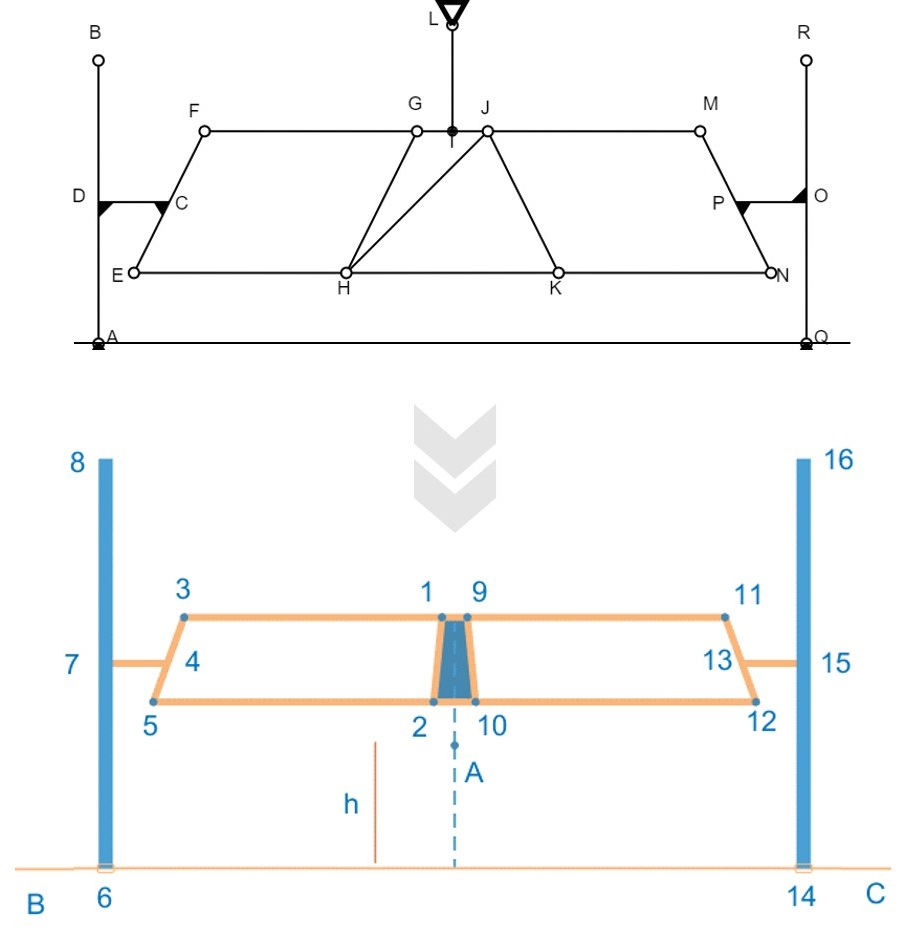
\includegraphics[width=1.0\linewidth]{figs/05/sim/1}
	\caption{Simulated Model}
	\label{model_schematic}
\end{figure}

Based on the Autodesk ForceEffect model designed previously, the suspension model was implemented in MATLAB. It has 20 points -- 3 of them fixed, A, B, C -- that define the bars. There are only three types of links in the model: articulations, weld and slider. 

The constraint equations that define this model can be summarized in these types (the examples have been taken from the model in Figure \ref{model_schematic}):

\marginnote{$x_{i}$ is the x coordinate of the point i\\
$y_{i}$ is the y coordinate of the point i\\
$L_{a\,b}$ is the length of the bar $a$-$b$}
\begin{itemize}
\begin{itemize}
\item Bar $\hspace{1.25cm}(x_{1}-x_{3})^{2}+(y_{1}-y_{3})^{2}-L_{1\,3}^{2}=0$

\item Triangle  \begin{aligned}
(x_{1}-x_{2})^{2}+(y_{1}-y_{2})^{2}-L_{1\,2}^{2}=0\\
\hspace{0.5cm}(x_{1}-x_{9})^{2}+(y_{1}-y_{9})^{2}-L_{1\,9}^{2}=0\\
\hspace{0.5cm}(x_{2}-x_{9})^{2}+(y_{2}-y_{9})^{2}-L_{2\,9}^{2}=0
\end{aligned}

\item Welded \begin{aligned}
(x_{6}-x_{7})(x_{4}-x_{7})+(y_{6}-y_{7})(y_{4}-y_{7})-L_{6\,7}L_{4\,7}\cos(90)=0\\
\hspace{0.5cm}(x_{6}-x_{7})(y_{4}-y_{7})-(y_{6}-y_{7})(x_{4}-x_{7})-L_{6\,7}L_{4\,7}\sin(90)=0
\end{aligned}

\item Slider $\hspace{0.75cm}(x_{6}-x_{B})(y_{B}-y_{C})-(y_{6}-y_{B})(x_{B}-x_{C})=0$
\end{itemize}
\end{itemize}

Each of these constraint equations is denoted as $\Phi(\vec{g},t)$, since depend in the vector of the coordinates $\vec{g}$ and the time $t$.

In Figure \ref{model_schematic} only 16 moving and 3 fixed points have been represented. The model will be completed with the introduction of the tilting actuation and the driver model. In total there will be 20 moving points and 3 relative coordinates (angles), which make a total of \textbf{43 unknown coordinates}.
\[\vec{g}=\begin{bmatrix} x_{1}\quad y_{1}\quad x_{2}\quad ... \quad x_{20}\quad y_{20} \quad \theta \quad \gamma \quad \phi \end{bmatrix}_{43x1}\]
\[\Phi(\vec{g},t)_{42x1}\] \[\Phi_g(\vec{g},t)_{42x43}\quad with \quad \Phi_g(\vec{g},t)_{i,j}=\frac{\partial \Phi_{i}}{\partial x_{j}}\]

Note that the size of the coordinates vector (unknowns) is bigger than the number of equations in the system ($42\rightarrow43$). This is due to the fact that one of the coordinates will be degree of freedom, and therefore a known value.

Due to the geometry of the model, it is impossible to put one fixed articulation in each wheel's point of contact with the ground. Instead, one of these two links has to be modified into an articulated slider. Another alternative was the implemented design, with a fixed rotation point and one articulated slider on each wheel. With this decision, the model behavior is completely identical  --symmetrical-- on both sides.

From now on we will refer as \textbf{inner wheel} to the wheel closer to the center of rotation of the trajectory and as \textbf{outer} to the other one. This notation will be alternated with left and right wheels for inner and outer.


\newpage
\subsection{Kinematic Simulations}

The goal of the kinematic simulations is to find the best geometry for stability during the tilting motion, that is, to design the front suspension so that the inner wheel should maintain as vertical as possible, so the outer wheel.

The degree of freedom $z$ of the model is the rotation angle $\phi$ that the body forms with the vertical axis. The vector of coordinates $\vec{g}$ is formed by the $x$ and $y$ coordinates of the 20 points. Other extra variables, angles and distances of interest are also included in the vector $\vec{q}$. As stated previously, to study the motion of a system three problems have to be solved, in this order:

\begin{itemize}
\begin{itemize}
\item Position Problem

\marginnote{Position Problem: \\Input $z$; Unknown $g$}
Given a value for the degree of freedom $z=\phi$, the vector of coordinates is calculated solving the system of non-linear equations $\Phi$. The Newton-Raphson method is used to solve the equations:
\[\Phi(\vec{g}+\Delta\vec{g},t) \approx \Phi(\vec{g},t)+\Phi_{\vec{g}}(\vec{g},t)\Delta\vec{g} \approx 0\] where the $\Phi_{\vec{g}}$ is the Jacobian of the constraint equations. Through a iterative process, the values of the coordinates are calculated: \[\Phi_{\vec{g}}(\vec{g}_{i},t)(g_{i+1}-g_{i})=-\Phi(g_{i},t)\]

\item Velocity Problem

\marginnote{Velocity Problem: \\Input $g,\dot{z}$; Unknown $\dot{g}$}
The derivative of the constraint equations is also null:
\[\frac{d}{dt}\Phi(\vec{g},t)=\Phi_{\vec{g}}\,\dot{\vec{g}}+\Phi_{t}=0\]
where $\Phi_{t}$ is the partial derivative of the constraint equations with respect to time $t$. The position of the system is known for each time $t$, so the matrix  $\Phi_{\vec{g}}$ and $\Phi_{t}$ are known, which gives the values of the velocity $\dot{\vec{g}}$: \[\Phi_{\vec{g}}\,\dot{\vec{g}}=-\Phi_{t}\]

\item Acceleration Problem

\marginnote{Acceleration Problem: \\Input $g,\dot{g},\ddot{z}$; Unknown $\ddot{g}$}
Following the same logic, the vector of accelerations is obtained:
\[\frac{d^2}{dt^2}\Phi(\vec{g},t)=\Phi_{\vec{g}}\,\ddot{\vec{g}}+\dot{\Phi}_{\vec{g}}\,\dot{\vec{g}}+\dot{\Phi}_{t}=0\]. If this equation is rearranged, the only unknown is the vector of accelerations $\ddot{\vec{g}}$: \[\Phi_{\vec{g}}\,\ddot{\vec{g}}=-\dot{\Phi}_{\vec{g}}\,\dot{\vec{g}}-\dot{\Phi}_{t}\]

\end{itemize}
\end{itemize}

\subsection{Dynamic Simulations}

Once the kinematic problem has been solved, the dynamic of the system can be studied. From the principle of virtual work: \[\delta W_{inertia} + \delta W_{external} =0 \] Applying this theorem in function of the vector of natural coordinates $g$: \begin{equation}
\delta \vec{g}^{T}\,M\,\ddot{\vec{g}}+\delta \vec{g}^{T}\,Q=0
\label{dynamic}
\end{equation} where $M$ is the mass matrix and $Q$ the vector of generalized forces.
\begin{marginfigure}
	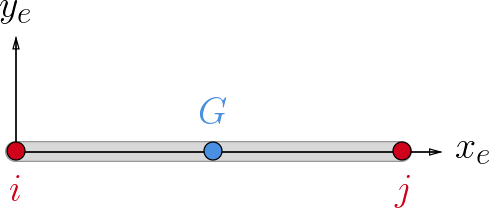
\includegraphics[width=1.0\linewidth]{figs/05/bar}
	\caption{Element of the model}
\end{marginfigure}
To build $M$, each element's $M_{e}$ is calculated first, and its inserted in the corresponding cells of the $M$ matrix. 
\[M_{e}=\begin{bmatrix}
m+a-2b_{x} & 0 & b_{x}-a & -b_{y} \\
	& m+a-2b_{x} & b_{y} & b_{x}-a \\
	 & & a & 0 \\
	 sim. & & & a
\end{bmatrix}\]
with
\[a=\frac{I_{i}}{L_{i\,j}^2} \quad b_{x}=\frac{m\, ^{e}x_{G}}{L_{i\,j}} \quad b_{y}=\frac{m\, ^{e}y_{G}}{L_{i\,j}} \quad m=\int_{V}{dm}\]
\[I_{i}=\int_{V}{(^{e}x^{2}+\,^{e}y^{2})dm \quad ^{e}x_{G}=\frac{1}{M}\int_{V}{^{e}x\,dm \quad ^{e}y_{G}=\frac{1}{M}\int_{V}{^{e}y\,dm\]

The matrix $Q$ is build in the same way, but accounts for the external forces in the system, for example, the torque from a motor. For any force $F$ in the model:
\[Q_{F}=\frac{1}{L_{i\,j}}
\begin{bmatrix}
L_{i\,j}-\,^{e}x & \,^{e}y \\
\,^{e}y  & L_{i\,j}-\,^{e}x \\
^{e}x & ^{e}y \\
-\,^{e}y & ^{e}x
\end{bmatrix}
\begin{bmatrix}
F_{x} \\ F_{y}
\end{bmatrix}\]

The matrix $M$ and $Q$ are therefore known. The values of the coordinates vector $\vec{g}$ can be expressed as a function of the degrees of freedom $z$ as $\vec{g}=f(z)$ where \[\dot{\vec{g}}=\frac{\partial f}{\partial z}\dot{z}=R\,\dot{z} \hspace{1cm} \ddot{\vec{g}}=R\,\ddot{z}+\dot{R}\,\dot{z}\] Returning to the equation (\ref{dynamic}): 
\begin{eqnarray*}
\delta \vec{g}^{T}(M\ddot{\vec{g}}-Q)=0\\
\delta z^{T}R^{T}(M\ddot{\vec{g}}-Q)=0\\
R^{T}(M\ddot{\vec{g}}-Q)=0 \\
R^{T}M\ddot{\vec{g}}=R^{T}Q\\
R^{T}MR\ddot{z}=R^{T}Q-R^{T}M\dot{R}\dot{z}
\end{eqnarray*}
Thus the acceleration of the degrees of freedom is obtained when mass and external forces are applied. 

\subsection{Torque Calculation}

It must be pointed out that in this thesis, the only variable of interest is the torque requirement from the motor. In order to get that variable a different perspective is necessary. 

Once again from equation (\ref{dynamic}), the Lagrange multipliers ($\lambda$) are introduced. There is one $\lambda$ per constraint equation in the model, and depending on their equation their meaning changes, but overall are related to the reactions between elements. 
\begin{equation}
M\ddot{\vec{g}}-Q+\Phi_{g}^{T}\lambda=0 \label{lagrange}
\end{equation}
For getting the value of the motor torque, a known tilting angle trajectory $\phi_{c}(t)$  has to be imposed:\begin{equation}
\Phi=\phi(t)-\phi_{c}(t) \label{motor_torque}
\end{equation}
For the sake of the programmer, once the kinematics have been solved, it is quite disturbing to change the system of equations again, introducing a new time depending equation. If only the motor torque is needed, a particular method to get it can be developed.

First, let us consider that the tilting angle $\phi$ is part of the coordinates vector $\vec{g}$ as: \[\vec{g}=\begin{bmatrix}
x_{1}\quad y_{1}\quad x_{2}\quad ... \quad x_{20}\quad y_{20} \quad \theta \quad \gamma \quad \phi
\end{bmatrix}\]

It was already verified that: \[M\ddot{\vec{g}}-Q+\Phi_{g}^{T}\lambda=0\] \[\lambda=\Phi_{g}^{H}(M\ddot{\vec{g}}-Q)\] Inserting the equation (\ref{motor_torque}) does not change the terms $M\ddot{\vec{g}}-Q$ in equation (\ref{lagrange}). It only expands the Jacobian $\Phi_{g}$ with a row of zeros and a one:\[\begin{bmatrix}\Phi_{g}\end{bmatrix} \quad\rightarrow\quad \left[\begin{array}{ccccc}
& & \Phi_{g} &  & \\ \hline
0 & 0 & ... & 0 & 1 \\
\end{array}	\right]\]
Returning to equation (\ref{lagrange}), the lagrangian terms becomes: \[\begin{bmatrix}
\Phi_{g}^{T} \end{bmatrix}\begin{bmatrix}\lambda_{1}\\ \lambda_{2} \\ ... \\  \lambda_{42}  \end{bmatrix}\quad\rightarrow\quad \left[\begin{array}{c|c} & 0 \\ & 0 \\ \Phi_{g}^{T}(1:42,:) & ... \\ & 0 \\ \hline \Phi_{g}^{T}(43,:) & 1 \\ \end{array}	\right]\begin{bmatrix}\lambda_{1}\\ \lambda_{2} \\ ... \\  \lambda_{42} \\ \lambda_{43} \end{bmatrix}\] Calculating the product of this new lagrangian term and considering that the mass and external forces terms do not change: 
\[M\ddot{\vec{g}}-Q+\Phi_{g}(1:42,:)^{T}\lambda=0\] \[\Phi_{g}^{T}(43,:)  \begin{bmatrix}
\lambda_{1} & \lambda_{2} & ... &  \lambda_{42} \end{bmatrix}^{T} + \lambda_{43}=0\] \[M_{t}=\lambda_{43}=-\Phi_{g}^{T}(43,:) \begin{bmatrix} \lambda_{1} & \lambda_{2} & ... &  \lambda_{42} \end{bmatrix}^{T}\]

\newpage
\subsection{MATLAB Simulations}
\textbf{Model}

\begin{figure}
	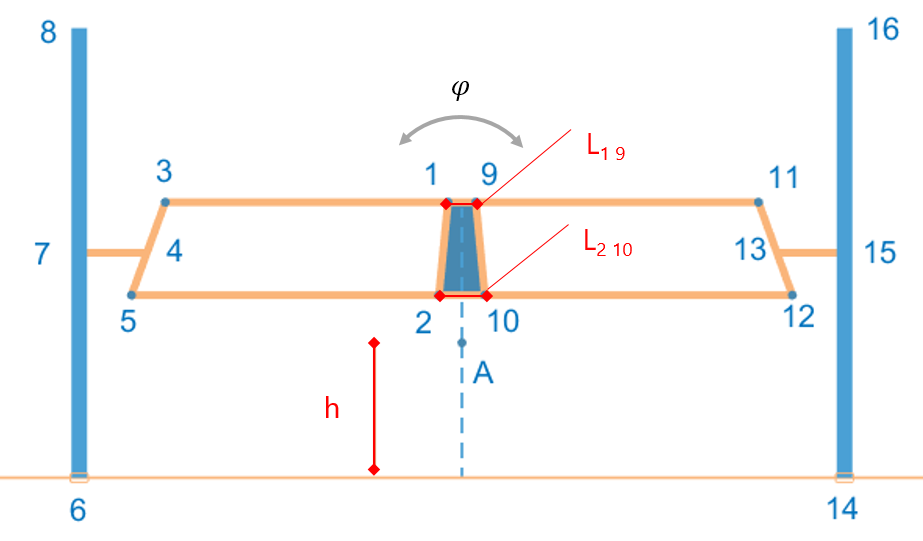
\includegraphics[width=1.0\linewidth]{figs/05/sim/Picture2}
	\caption{Model}
\end{figure}
The model has a pre-established constraints, due to the selection of some components. That is the reason why there are some fixed dimensions:
\begin{itemize}
\begin{itemize} \itemsep -15pt
 \item Wheel Radius
 \item Vehicle Track
 \item Kingpin angle
 \item Hub width and height
 \item Wishbone arms horizontal in steady state
\end{itemize}
\end{itemize}
The \textbf{degree of freedom} is the body inclination $\phi$, based on the rotation point A, where the motor should be placed. For the kinematic simulations it will be established that: $\phi=(0\,-\,30)\,\degree;\quad \dot{\phi}=1 rad/s;\quad \ddot{\phi}=0 rad/s^{2}$

\textbf{Kinematics}

We will study the motion of the system with varying parameters. The only parameters left to determine are the \textbf{position of the motor} --height $h \in (0-600) mm$-- and the \textbf{width of the body in the suspension} --$L_{1\,9},\,L_{2\,10} \in (0-300) mm$--, which will initially cover those ranges.

The model is fixed to some dimensions, and its \textbf{tilted to the maximum possible angle}. The inclination of the body and the wheels is recorded and saved. Then both the left and right wheels angle is compared with the body angle. This data is the \textbf{fitted into a linear regression} and its slope and quadratic error are saved for later analysis.
\begin{figure*}
	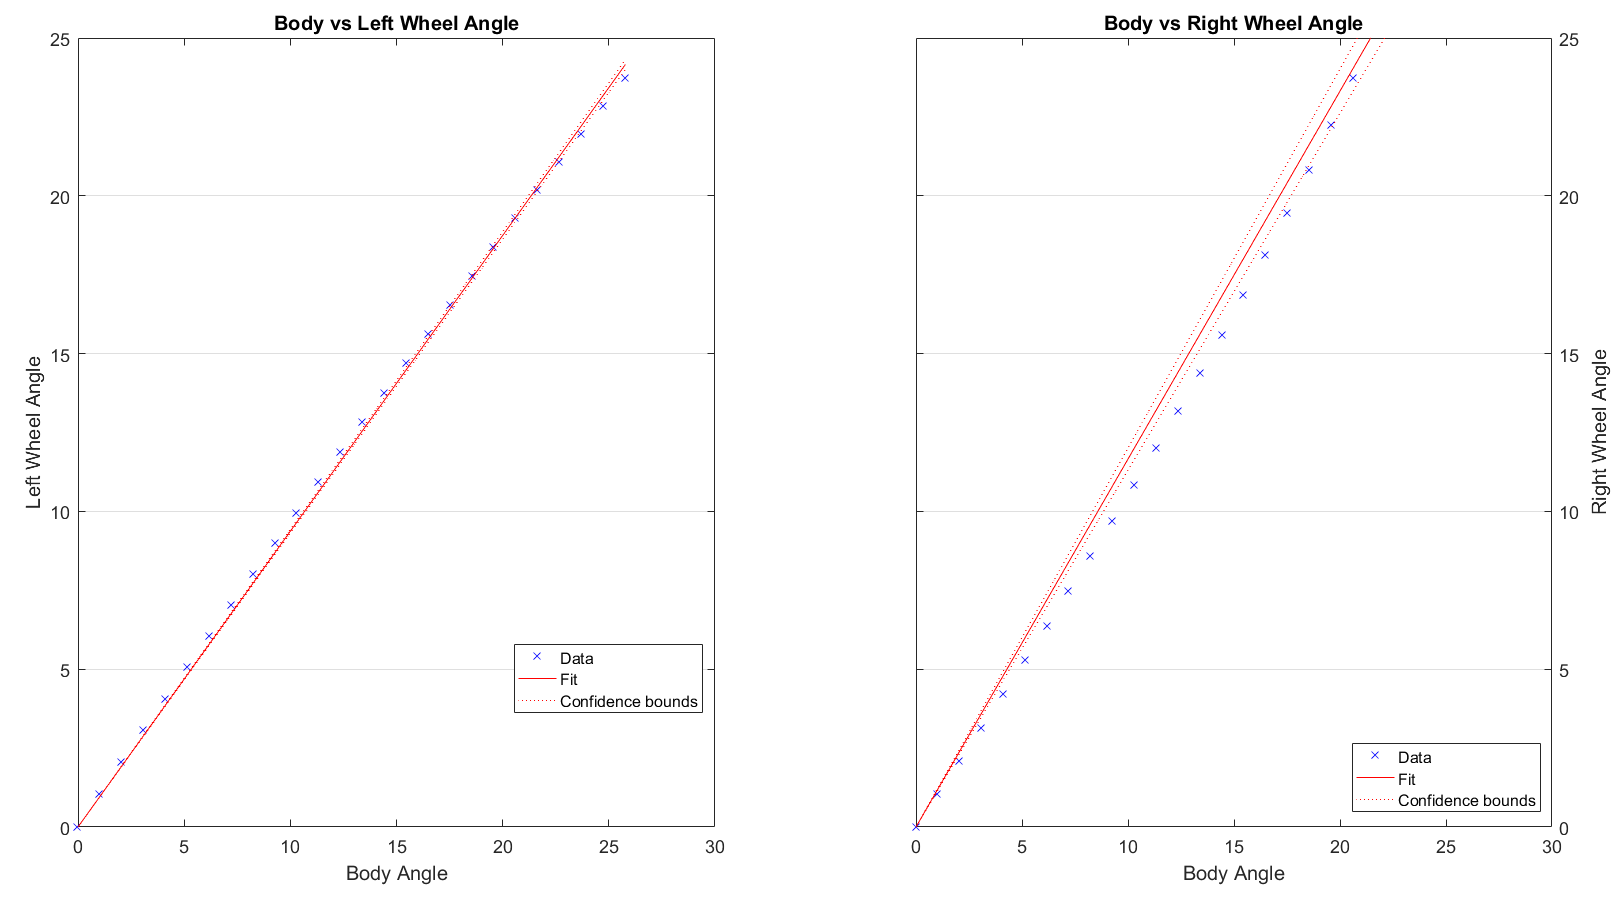
\includegraphics[width=1.0\linewidth]{figs/05/sim/Relations}
	\caption{Left (inner) and right (outer) wheels angle versus the body angle during a tilting motion}
\end{figure*}

After simulating the mechanism with different geometric constraints (54900 combinations), some conditions were applied to find the most suitable geometry:
\begin{enumerate}\itemsep -8pt
 \item Ratio between the inner wheel inclination angle and the body leaning \textbf{$\phi_{inner\,to\,body}< 0.96$}
 \item The body width should have enough space for connecting the suspension arms \textbf{$L_{1\,9},\,L_{2\,10} > 30 mm$}
 \item The body should lean a minimum angle ($\phi_{max}>25\degree$)
 \item The rotation point should be located near to the body, in order to avoid the motor scraping against the ground or being too high.
\end{enumerate}
Applying these constraints a set of possibilities is obtained: 
\begin{table}[h!]
\centering
\begin{tabular}{ccc|ccccc}
	\\[20pt]
	h   & L_{1\,9} & L_{2\,10} & \phi_{max} & \phi_{left\,to\,body} & RSE_{left\,to\,body} & \phi_{right\,to\,body} & RSE_{right\,to\,body} \\ \hline
	260 & 31    & 61  & 0.4500   & 0.9530  & 0.0020  & 1.1560  & 0.0020\\
	260 & 61    & 101  & 0.4500   & 0.9592  & 0.0017 & 1.1397  & 0.0017\\
	250 & 31    & 61   & 0.4500   & 0.9534  & 0.0020 & 1.1598  & 0.0020\\
	\textbf{250} & \textbf{61}    & \textbf{101}  & \textbf{0.4500}   & \textbf{0.9596}  & \textbf{0.0017} & \textbf{1.1432}  & \textbf{0.0017}\\
	240 & 31    & 61   & 0.4500   & 0.9539  & 0.0019 & 1.1432  & 0.0019\\
	240 & 61    & 101  & 0.4500   & 0.9600  & 0.0017 & 1.1643  & 0.0017\\
	230 & 31    & 61   & 0.4499   & 0.9543  & 0.0019 & 1.1730  & 0.0019\\ \hline  
	\end{tabular}
	%\\[20pt]
	\caption{Geometries remaining after applying the selection constraints}
	\label{selection}
\end{table}

\newpage
The selected geometry has been emphasized in the table \ref{selection} and represented in Figure \ref{selectedgeometry}. The motor should be located inside the body, at $230–260$ mm from the ground. The selection of $L_{1\,9}$ is clearly affected by the second constraint, it usually selects the lower bound (31 mm). Regarding the body geometry, the length $L_{1\,9}$ should be around 60 mm, while the length $L_{2\,10}$ should be around 100 mm. These values could be recalculated in case that the 60 mm separation between pins would not be enough. 

\begin{figure*}[h!]
	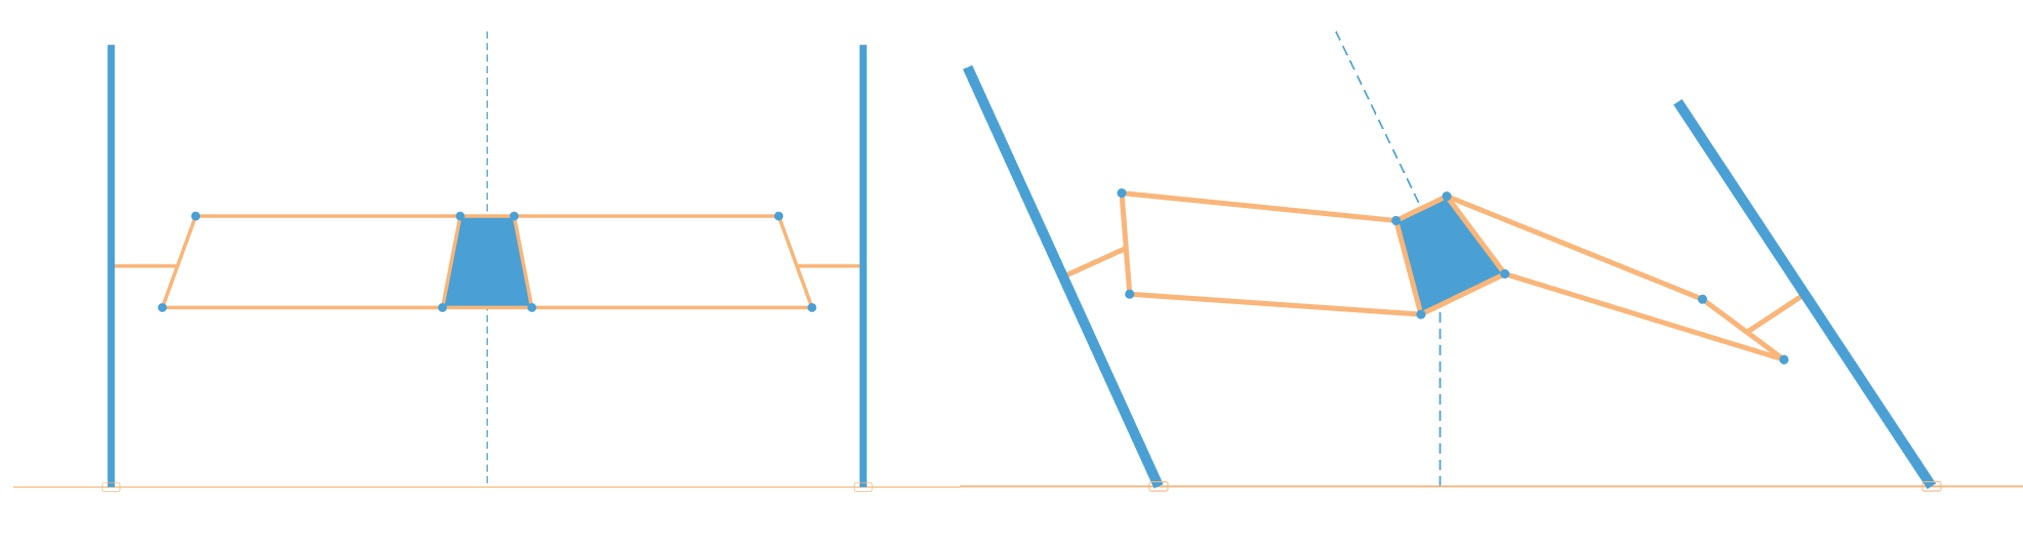
\includegraphics[width=1.0\linewidth]{figs/05/sim/4}
	\caption{Selected geometry}
	\label{selectedgeometry}
\end{figure*}

Other interesting conclusions can be extracted from the kinematic analysis. First, let us look at the value of $\phi_{max}$ (Figure \ref{phimax}) for all the possible combinations. 

We can notice that increasing the rotating point reduces the cases of high leaning angles. The lower the point A, the higher the leaning angle. In addition, ff the position of the rotating point is maintained constant ($h=constant$), that is, independently of the rotating point height, there exist a line where the dimensions $L_{1\,9}$ and $L_{2\,10}$ give the highest possible leaning angle. This line gives a body with a particular lateral edge. 

Indeed, the $\bar{12}$ edge would form 55$\degree$ with the horizontal in that optimum case. But reality is that the selection has to be based in a balance, going to the optimum in one dimension will mean worse values in the other dimensions.

In Figures \ref{phileft} and \ref{phiright} the values of $\phi_{inner}$ and $\phi_{outer}$ tell that independently from the rotating point height, the regions where there is a low inner wheel to body angle ratio are the same where there is a high outer wheel to body angle ratio. The selected point fall into a balanced zone between these two regions.

Finally, in Figure \ref{phirelation} the relation between the inner-wheel-to-body ratio and the outer -wheel-to-body ratio is represented. Out of curiosity, it is impossible to find a geometry in which simultaneously the inner and the outer wheel angle are lower than the body angle. When a ratio is below 1, the other ratio is always above 1, and vice versa.

\begin{figure*}
	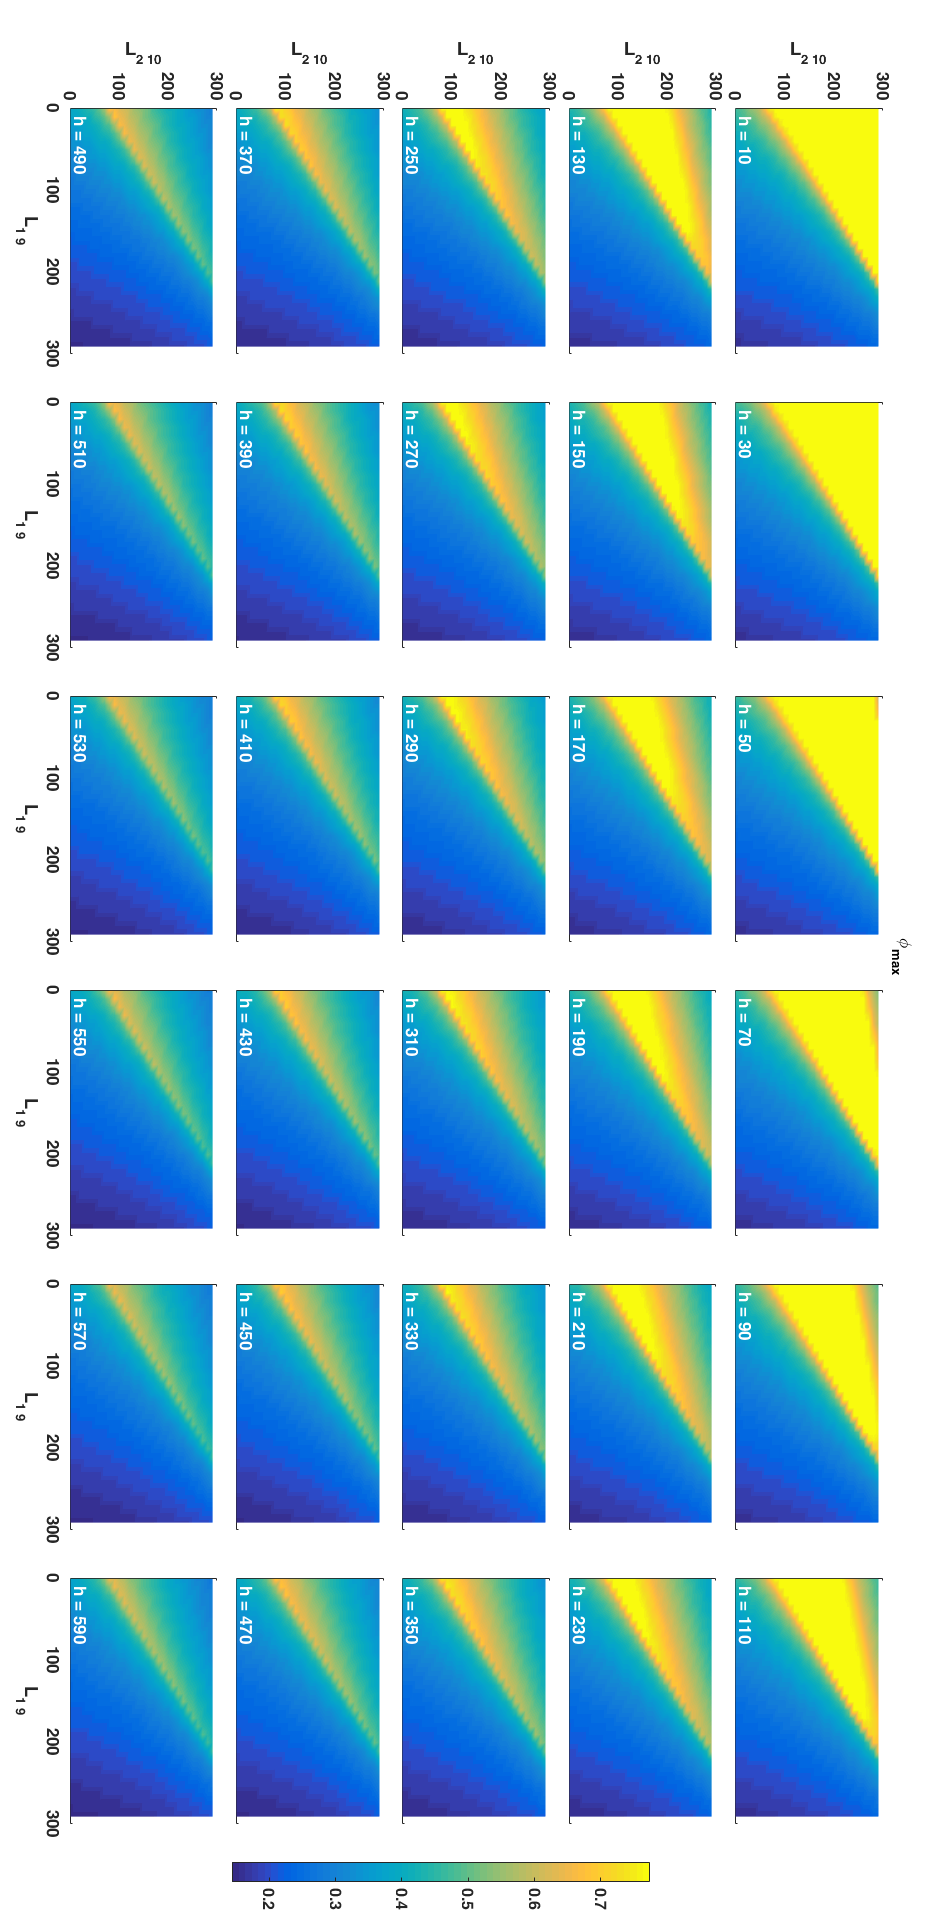
\includegraphics[width=1.0\linewidth]{figs/05/sim/phimax}
	\caption{Value of $\phi_{max}$ in function of $L_{1\,9}$ (x axis), $L_{2\,10}$ (y axis), and $h$ (different figures)}
	\label{phimax}
\end{figure*}

\begin{figure*}
	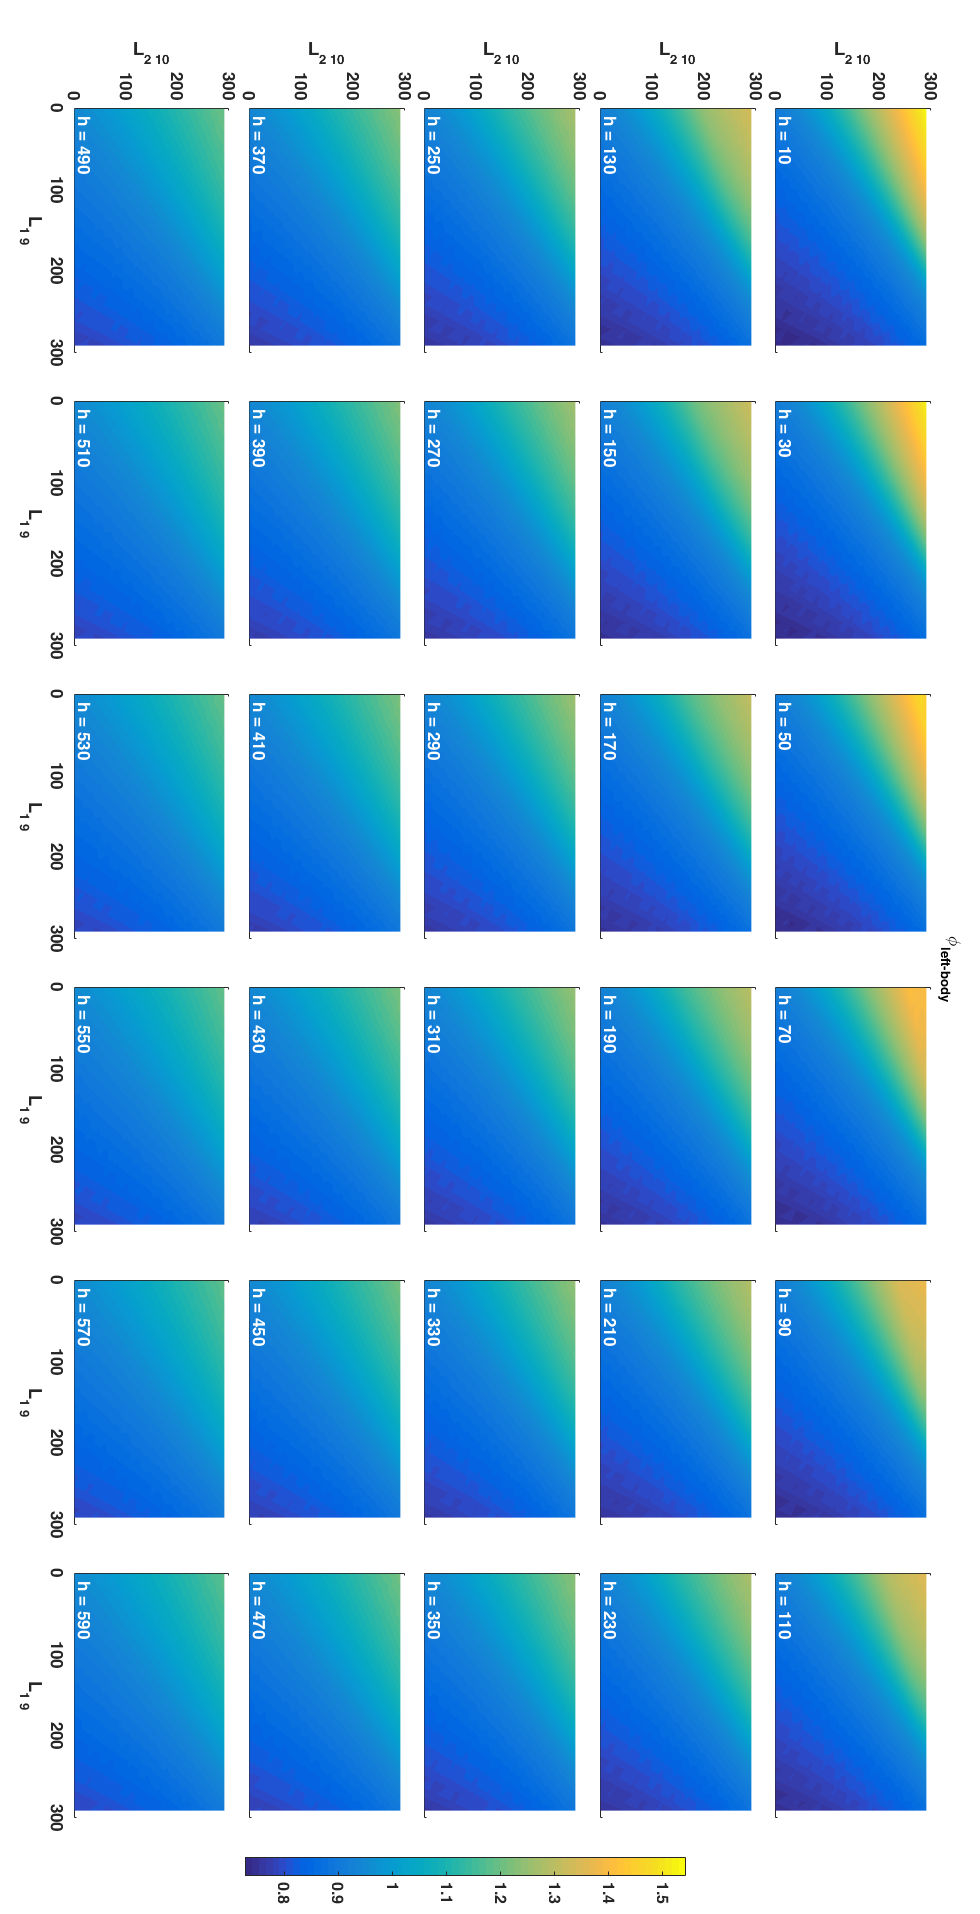
\includegraphics[width=1.0\linewidth]{figs/05/sim/phileft}
	\caption{Value of $\phi_{inner}$ in function of $L_{1\,9}$ (x axis), $L_{2\,10}$ (y axis), and $h$ (different figures)}
	\label{phileft}
\end{figure*}

\begin{figure*}
	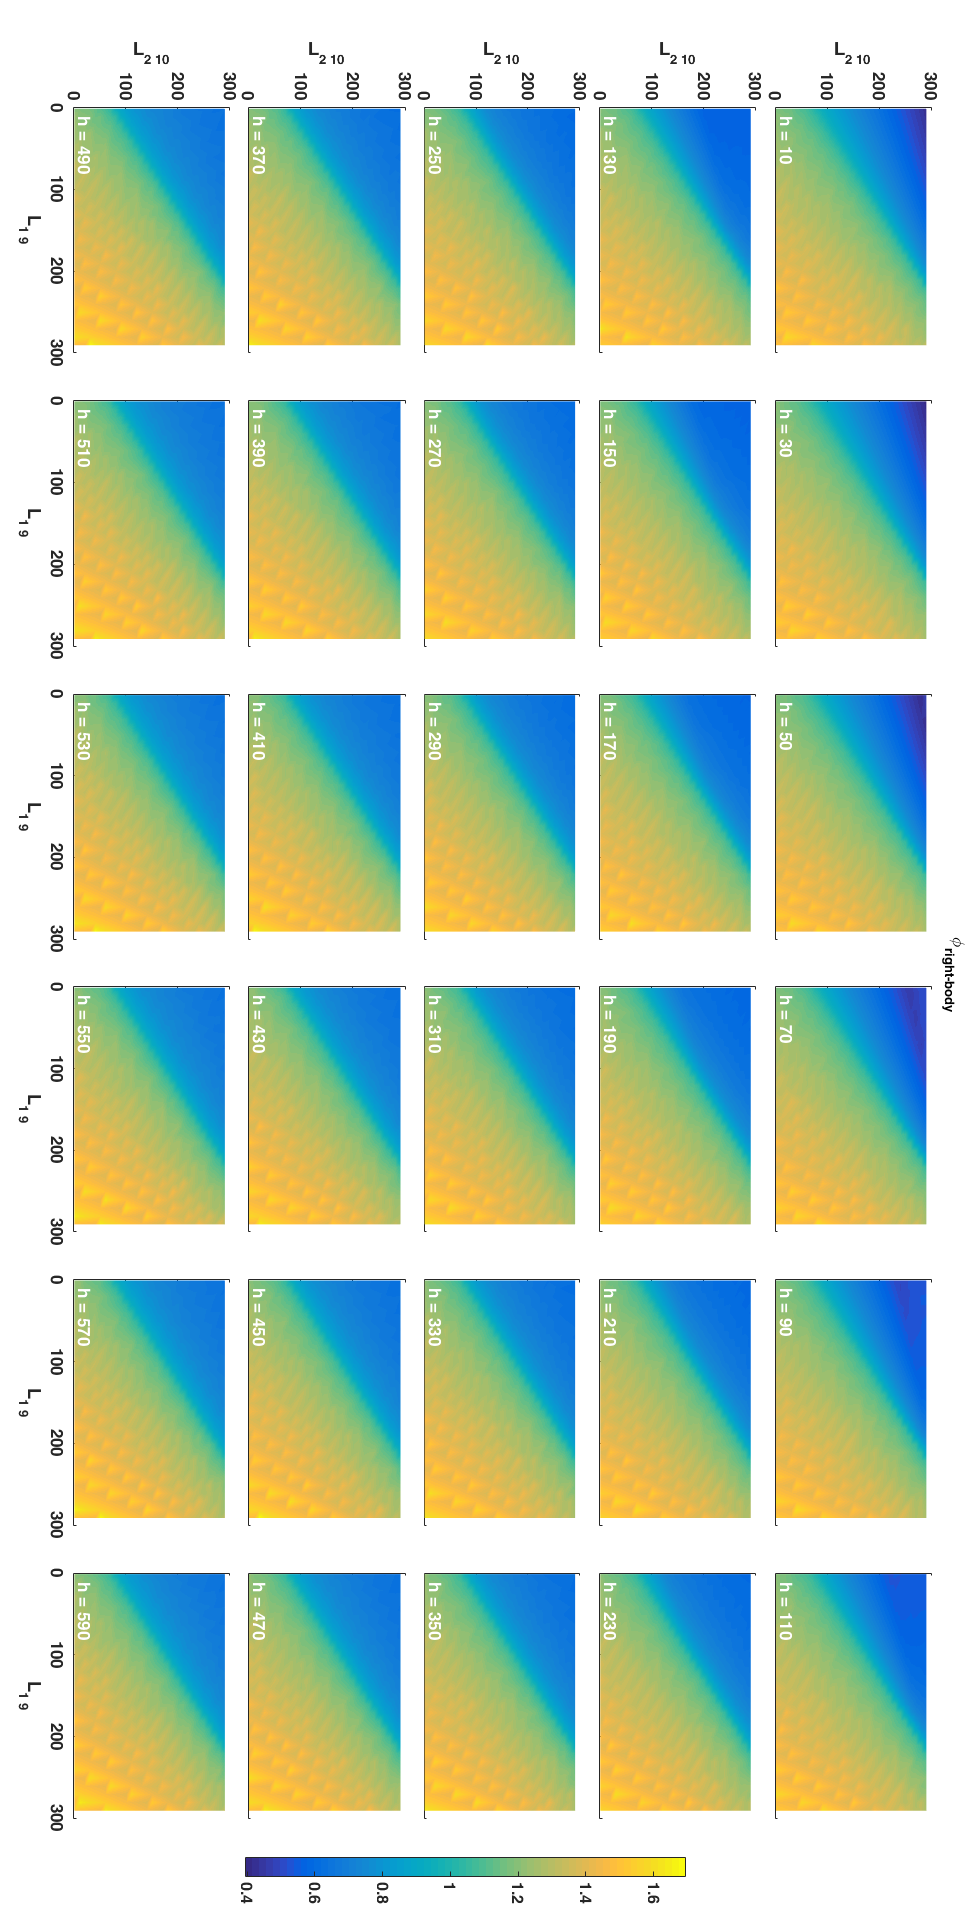
\includegraphics[width=1.0\linewidth]{figs/05/sim/phiright}
	\caption{Value of $\phi_{outer}$ in function of $L_{1\,9}$ (x axis), $L_{2\,10}$ (y axis), and $h$ (different figures)}
	\label{phiright}
\end{figure*}

\begin{figure}
	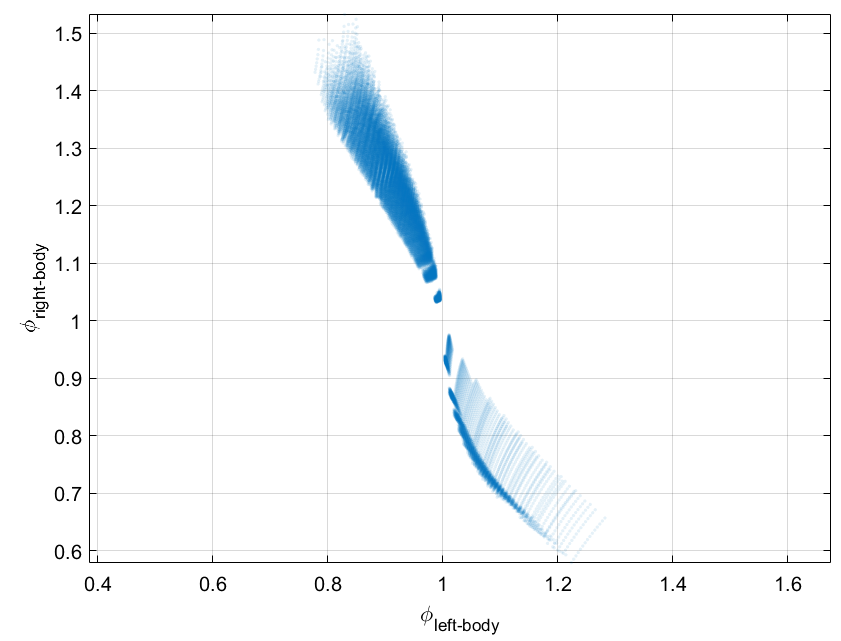
\includegraphics[width=1.0\linewidth]{figs/05/sim/PhiRelation}
	\caption{Ratio of angles on inclination $\phi_{inner\,to\,body}$ vs $\phi_{outer\,to\,body}$ in function of $L_{1\,9}$ (x axis), $L_{2\,10}$ (y axis). Each point represents a combination of the geometry}
	\label{phirelation}
\end{figure}

\textbf{Dynamics}

The dynamic analysis has been focused on the estimation of the necessary torque to maintain the body in vertical position. The worst case scenario for the motor is when the user gets on the vehicle. The motor will be able to return to the vertical position only if the torque requirement is lower than the maximum torque of the motor. On the contrary, inn a dynamic situation the forces on the vehicle will help the motor to return to the vertical position after a curve.

To carry out the dynamic simulation, the weight of each element is estimated with their material density and approximate dimensions. In addition, the weight of an standard (80kg) driver is include at a height on 1m (around the center of gravity).

Then, the model is forced to a known initial position ($\phi$ is the input) and the torque to return to the vertical position is calculated. For this step the expressions presented previously, based on the Lagrangian formulation, is used:\[M_{t}=\lambda_{m}=-\Phi_{g}^{T} \begin{bmatrix} \lambda_{1} & \lambda_{2} & ... &  \lambda_{20} \end{bmatrix}\]
The model was also slightly modified to include the tilting mechanism. The design B.4 was selected for this analysis, which consisted on a gear system attached between the motor and the lower suspension arms. Two different gear ratios were studied, with an increase of 1.5:1 and 4:1 in the motor torque:

\newpage
\begin{marginfigure}[5cm]
	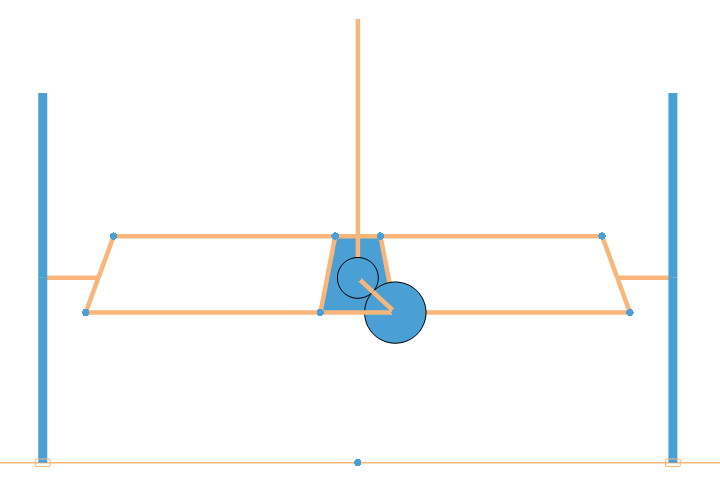
\includegraphics[width=1.15\linewidth]{figs/05/sim/gear15_2}
	\caption{Studied model with gear ratio=1.5}
\end{marginfigure}
\begin{marginfigure}[5cm]
	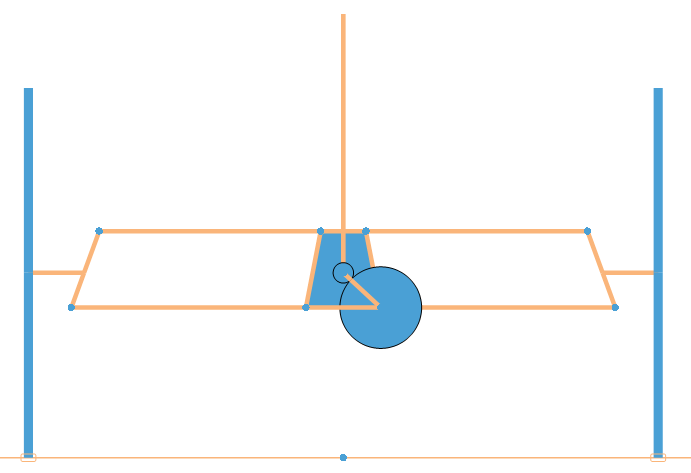
\includegraphics[width=1.15\linewidth]{figs/05/sim/gear4_2}
	\caption{Studied model with gear ratio=4}
\end{marginfigure}
\begin{figure}[h!]
	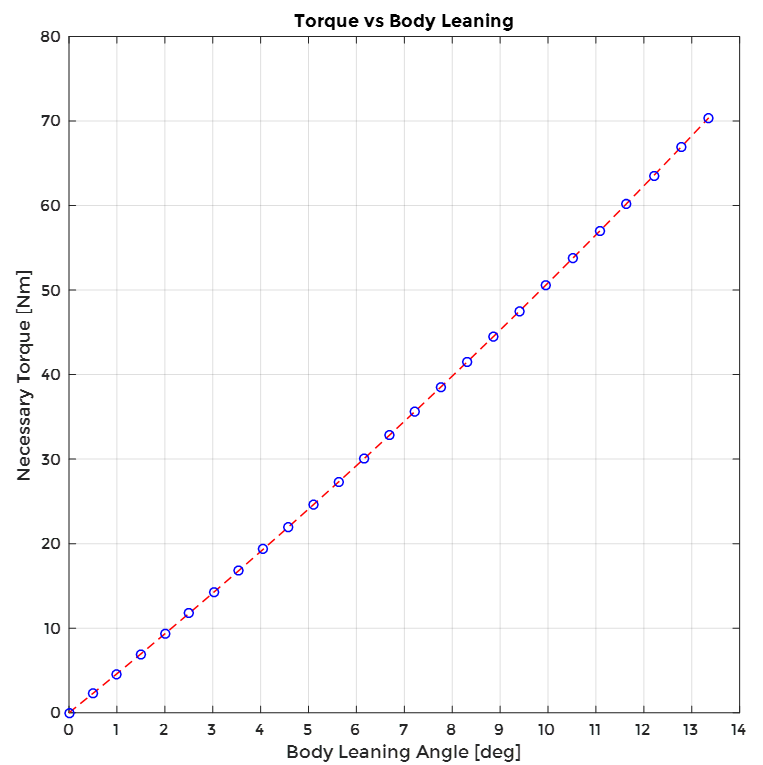
\includegraphics[width=0.95\linewidth]{figs/05/sim/gear15_1}
	\caption{Necessary motor torque to restore vertical position with gear ratio=1.5}
\end{figure}

\begin{figure}[h!]
	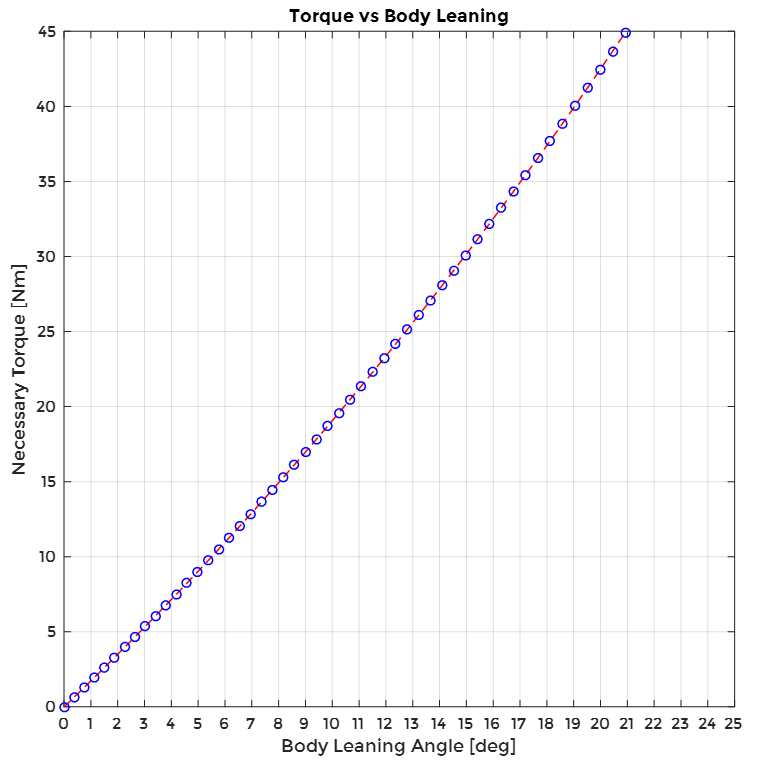
\includegraphics[width=0.95\linewidth]{figs/05/sim/gear4_1}
	\caption{Necessary motor torque to restore vertical position with gear ratio=4}
\end{figure}

For acceptable leaning angles (around 15\degree) there is torque requirement of 50Nm for the 1.5:1 gear ratio and of 15Nm for the 4:1 gear ratio. Let us study the characteristics of the available tilting motor to verify that this conditions are fulfilled.   

\newpage
\textbf{NIDEC 48R Motor}

The selected motor is a NIDEC 48R BLDC motor. Brushless DC motors do not require commutators and brushes, and have a long life, quietness, and high efficiency. It has a 144 ratio gear attached, which was customized for high-torque applications. The datasheet of the motor (without the gear) is included in the appendices. The rated power is 67W, with a nominal output torque $T_{r}$ of 0.2Nm and a current consumption of $I_{r}$ of 3.8A. In no load conditions, the output speed is $n_{0}=4460 1/min$, with a current consumption of 0.5A.
\begin{figure}[h!]
	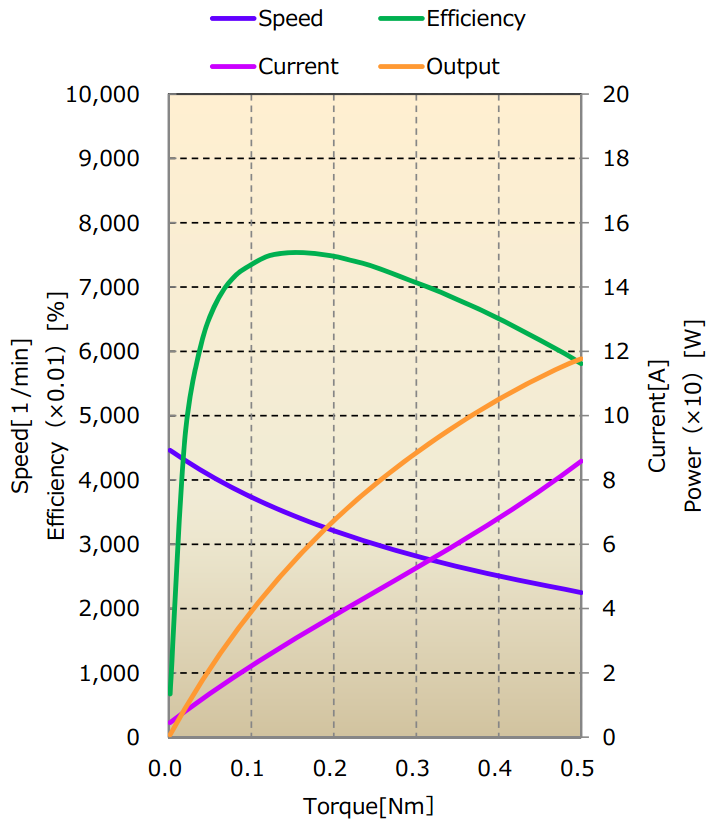
\includegraphics[width=0.85\linewidth]{figs/05/sim/motor}
	\caption{NIDEC 48R motor curves}
\end{figure}
\\\6
Considering these two situations --nominal and no load--, the curve torque vs current can be obtained. \[T=m\,I+n; \quad 0=0.5m + n; \quad 0.2=3.8m+n\] \[T=\frac{2I-1}{33}\] With a output ratio of 144 in the planetary gear, and limiting the \textbf{maximum current to 5A}, the maximum torque is \[T_{max}=144\frac{2·5-1}{33}\approx 40 Nm\] With an additional gear, the torque increases to \textbf{60Nm and 160Nm with 1.5 and 4 gears ratio} respectively. Therefore, the \textbf{motor is able to recover} from the considered situations. In the view of the results of the dynamic analysis, the gears between the motor and the suspension arms will be designed to have a \textbf{ratio of 2:1}.

\newpage
\section{Design}

The previous simulations have offered a better understanding of the motion of the front suspension and have helped to complete its geometry. In this section we will go through the design process for the different parts of the PEV.

\subsection{Tilting}
\begin{marginfigure}[5.5cm]
	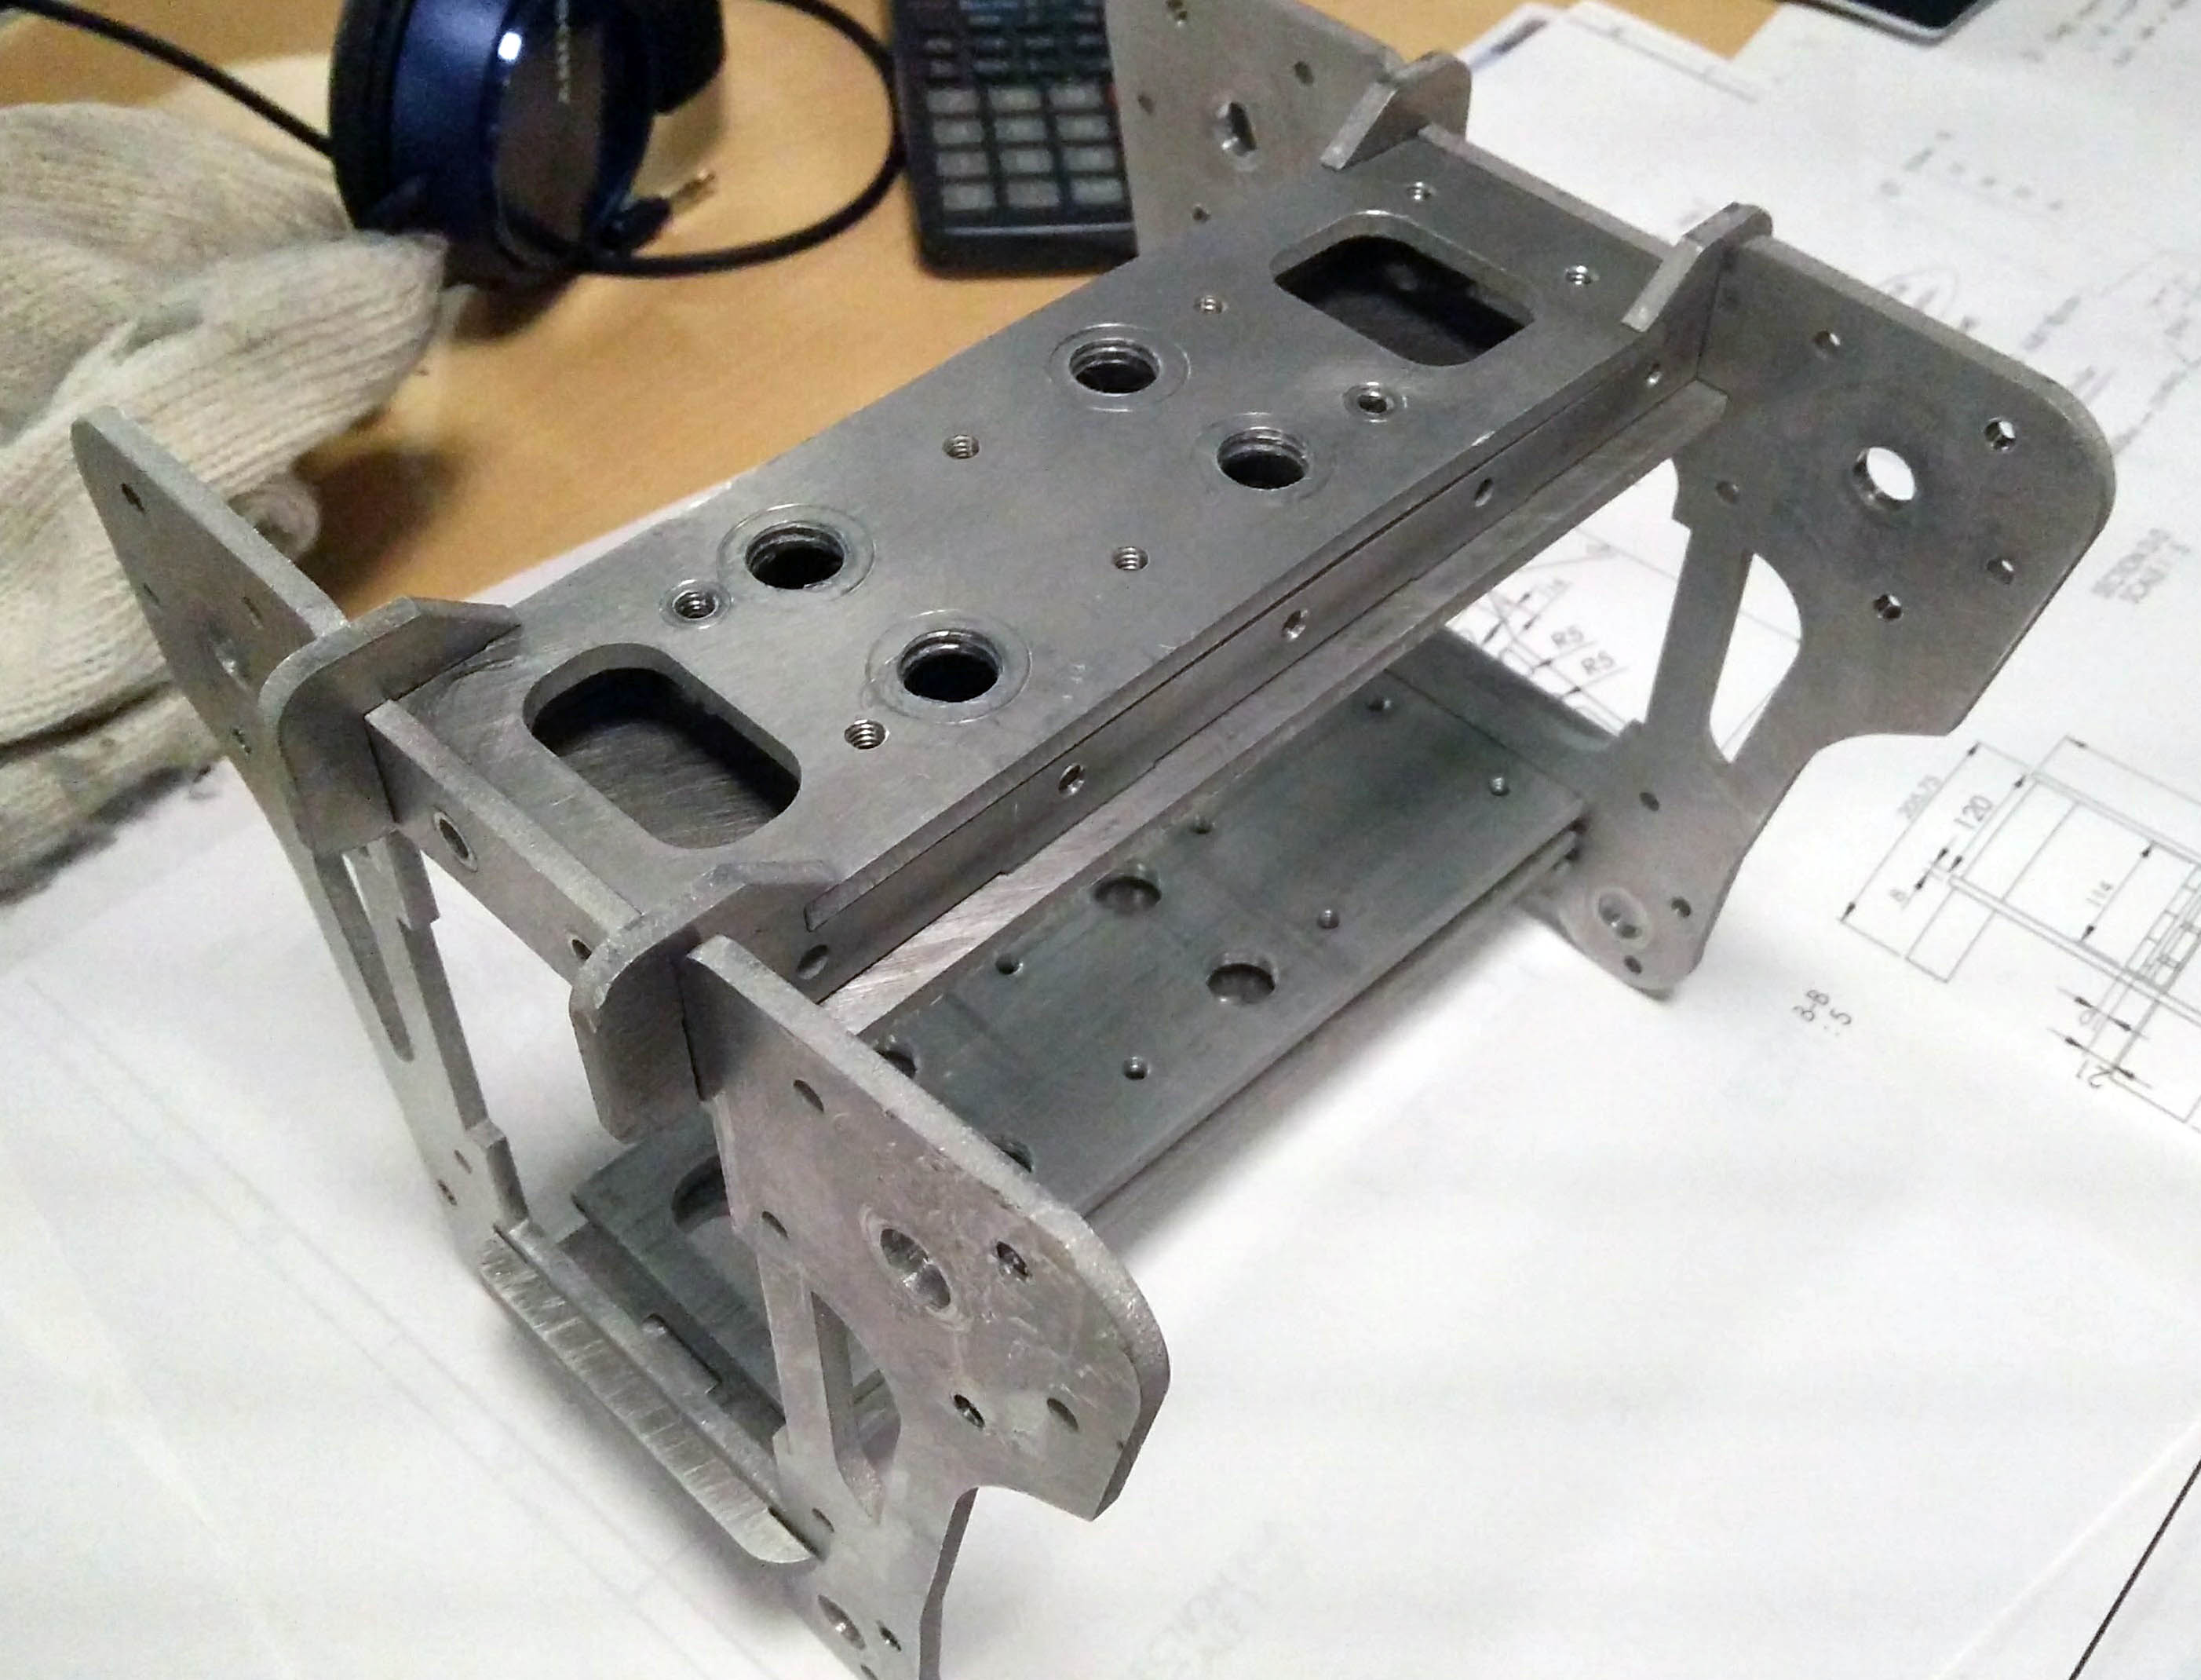
\includegraphics[width=1\linewidth]{figs/05/IMG_20161220_154842}
	\caption{Aluminum part to connect the frame and the suspension arms. The geometry fits with the output from the kinematic simulations (part upside down) }
\end{marginfigure}
For the tilting part some components were reused from other vehicles (wheels, suspension arms and hubs). The wheels are not perfectly suited for tilting vehicles, due to their narrow width. On the other side, the hubs determine the height of the suspension points in the frame, since in steady position the suspension arms are intended to remain parallel to the ground. 

The key point in the design of the tilting suspension was the selection of ball joints as articulations. Super-swivel ball joint rod ends were selected due to the 55$\degree$ angle of ball swivel, being able to accommodate more misalignment than any other externally threaded rod end. This high angle allowed the tilting of the vehicle up to 30$\degree$.

The rest of the joining components were purchased at McMaster.com --their cost has been summarized in the Ch.7: Cost Summary--, and their datasheets have been included in the appendices. The joining of the suspension arms and the frame was carried out by a aluminum part made of water jetted sheets of 1/8'=3.125 mm. This part followed the geometry extracted from the MATLAB simulations, having 60 mm and 100 mm between the upper and lower suspension points respectively.

\begin{figure}[h!]
	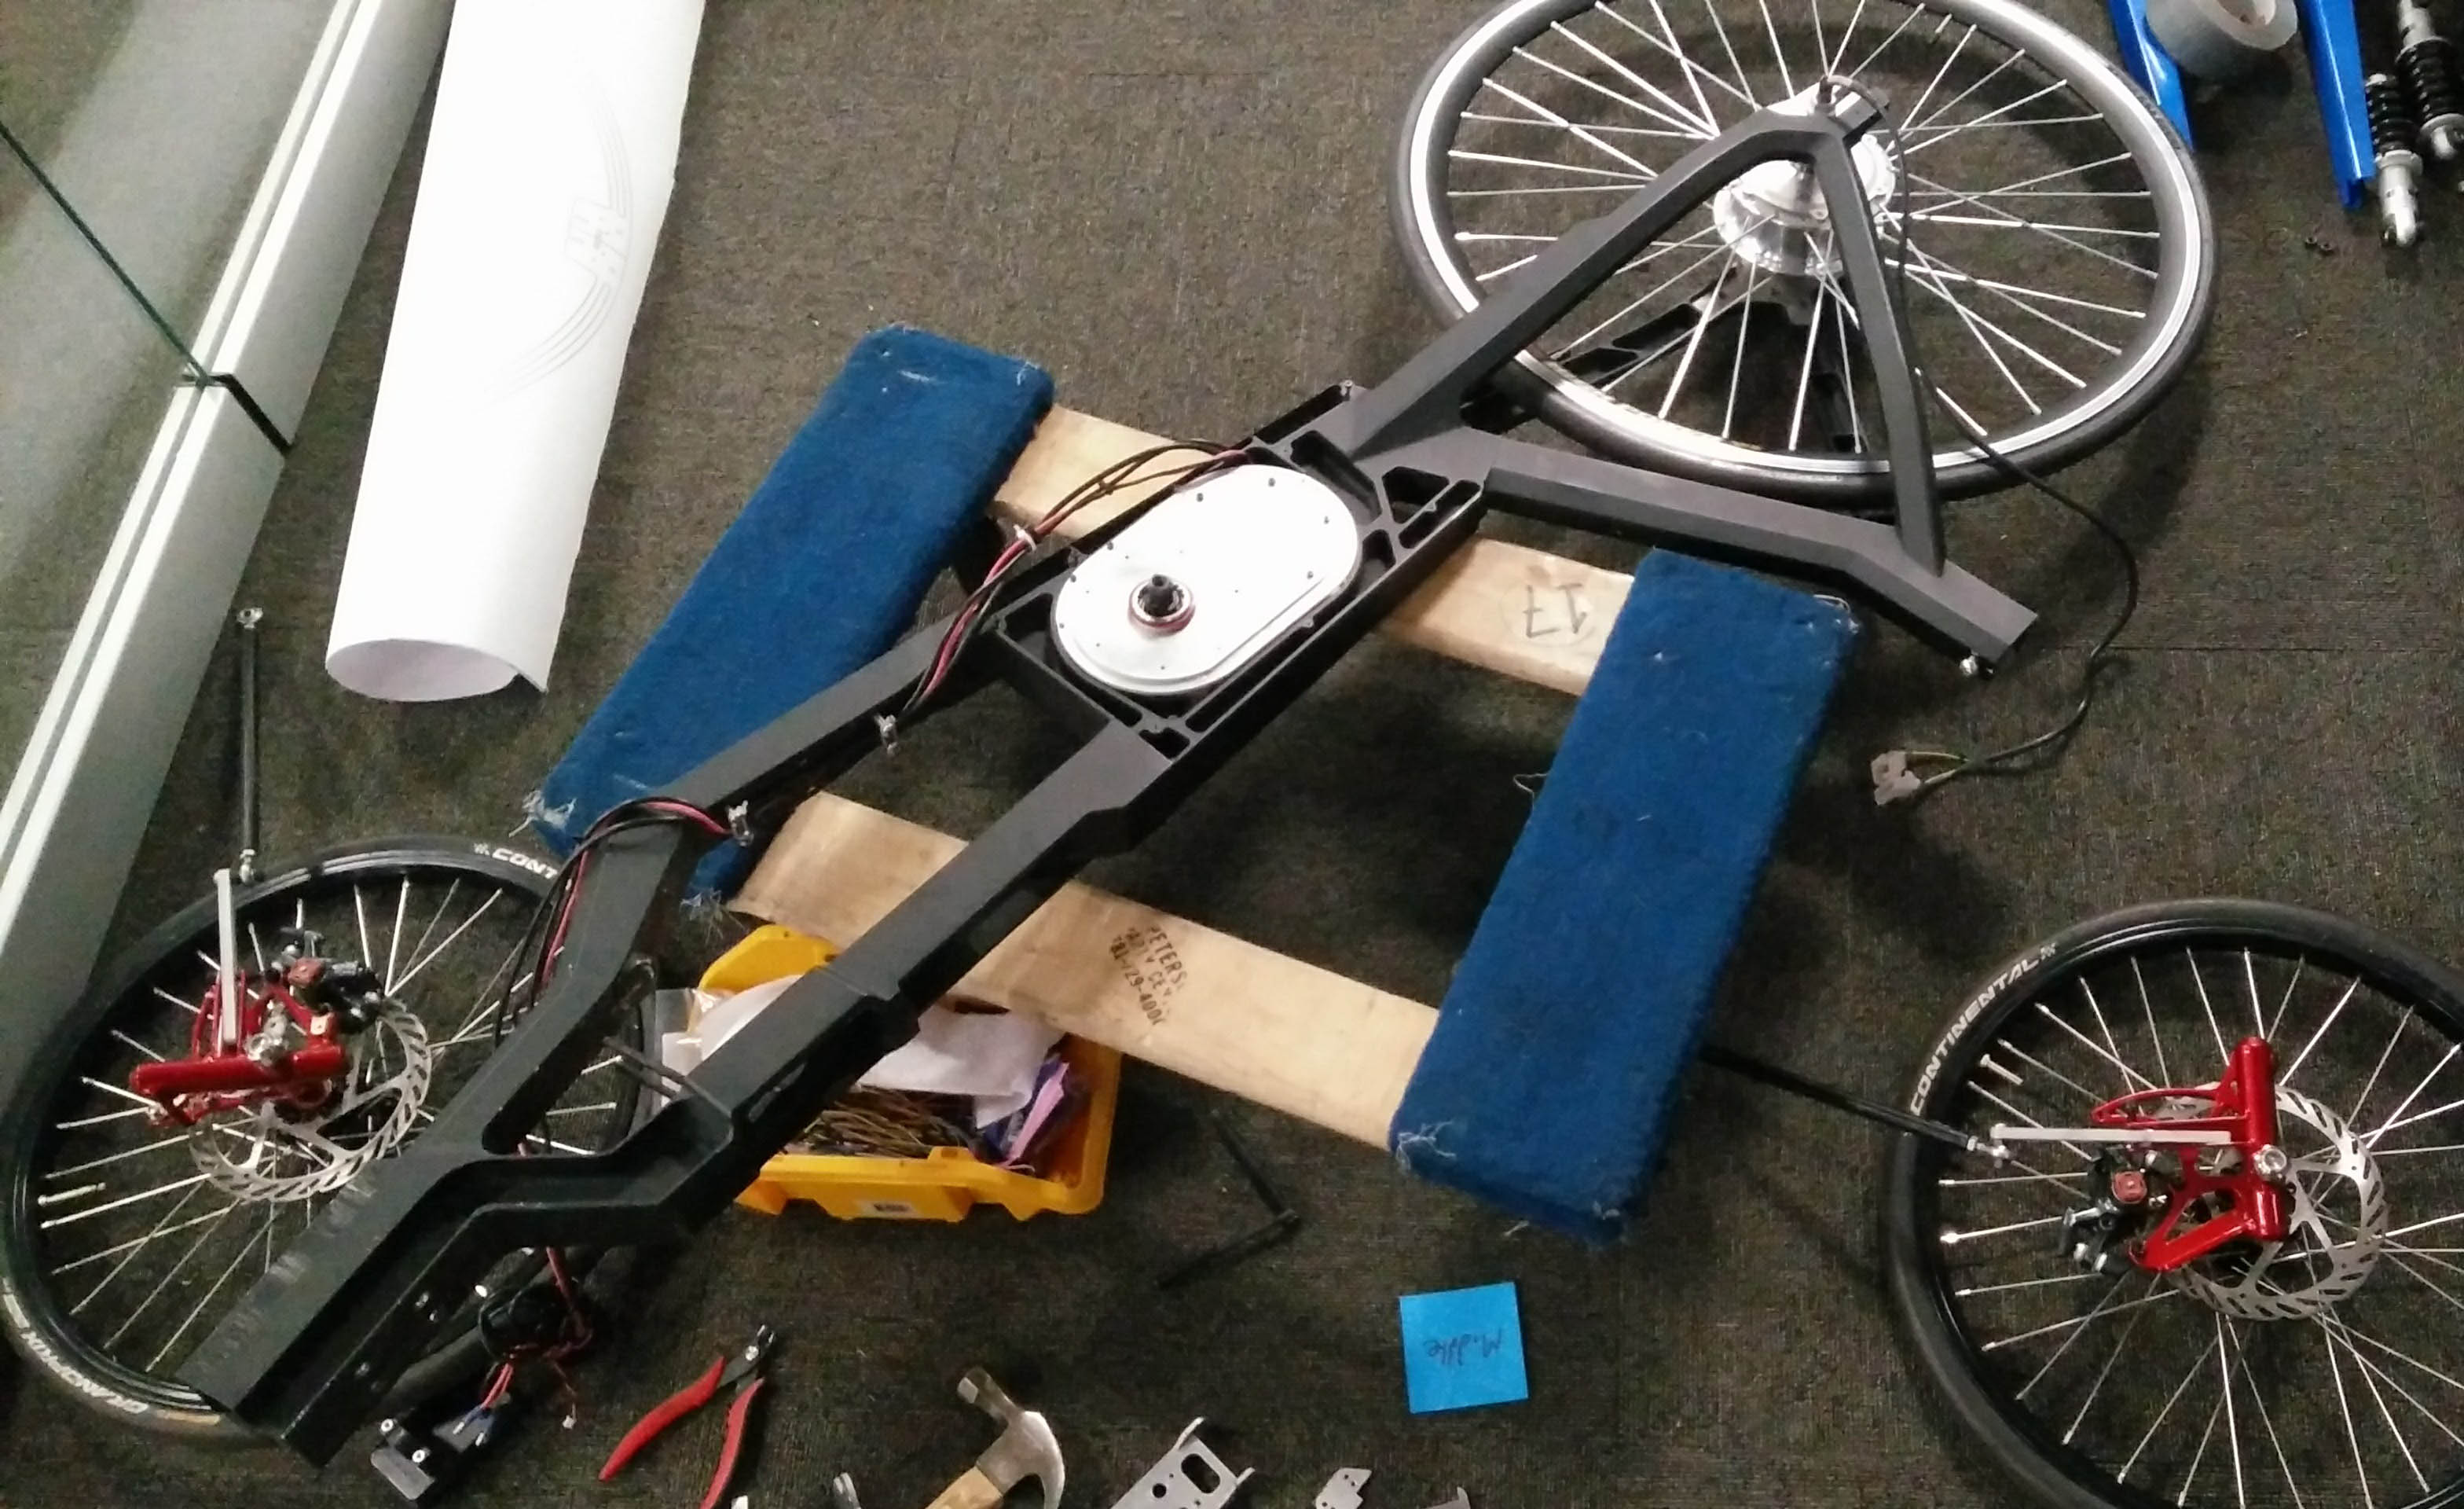
\includegraphics[width=1\linewidth]{figs/05/IMG_20161219_165930}
	\caption{Initial state of the PEV frame}
\end{figure}

\newpage
The gears were designed using a design table from excel\cite{gear} that was then imported to Solidworks. This table took into account all the parameters of the gears. As stated previously, the ratio of the gears was 2:1, with a width of 1/4'=6.35 mm and were fabricated with the water jet machine. The gears were inserted into the suspension arms by cutting them in half. This issue was due to the fact that the suspension arms were already fabricated and it was not possible to insert the gears in their position without breaking some parts.
\begin{table}[h!]
\centering
	\begin{tabular}{lll}
	\hline
	Half Width      & h  & 0.785 \\
	Addendum	    & a  & 1     \\
	Dedendum        & b  & 1.25  \\
	Fillet Radius   & e  & 0.38  \\
	Module          & m  & 1     \\
	Teeth           & z  & 20    \\
	Profile Shift   & s  & 0.25  \\
	Pressure Angle  & $\alpha$  & 0.349 \\
	Pitch Radius    & R  & 10    \\
	Base Radius     & R_{0} & 9.397 \\
	Addendum Radius & r_{a} & 11    \\
	Half Angle      & $\gamma$  & 0.093 \\
	Fillet Center   & v_{C} & -0.87 \\
	Fillet Center   & u_{C} & 1.506 \\
	\hline
	\end{tabular}
	%\\[20pt]
	\caption{Gear parameters}
\end{table}
\begin{marginfigure}[-2.75cm]
	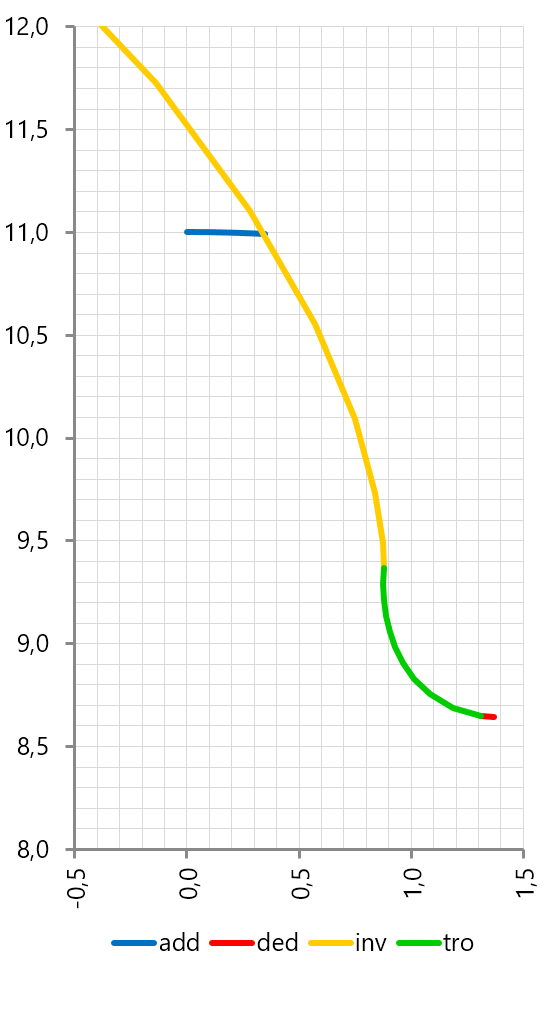
\includegraphics[width=1\linewidth]{figs/05/involute}
	\caption{Gear Design: Addendum, Involute, Trochoidal and Dedendum sections}
\end{marginfigure}
But far from meaning a problem, being able to put and remove the gears allowed to test the vehicle with and without tilting\ref{P1050722}. This modular advantage probed to be really useful, disassembling the gear and replacing a pair of shock absorbers allowed to test the vehicle with no tilting in a very straightforward way.

The frame was first modelled in Solidworks, as the baseline of the rest of the components. The non relevant parts were imported from online resources as GradCad, for example, the wheels. Once the frame was in Solidworks, the rest of the parts were designed and fabricated in the Media Lab's machine shop.

The assemble of the parts did not imply any problem. At this stage there was not steering system, so the wheels could rotate freely. This complicated a bit the tilting tests, since the wheels started rotating when the suspension moved. Nevertheless, the tilting mechanism worked satisfactorily and the inclination angles were as high as expected. 

The NIDEC motor was controlled with a driver connected to the Arduino board. The control strategy uses a PWM signal to command the speed of the motor and the position is controlled with a PID. In the electronics section a deeper explanation is included.

\begin{marginfigure}[-5cm]
	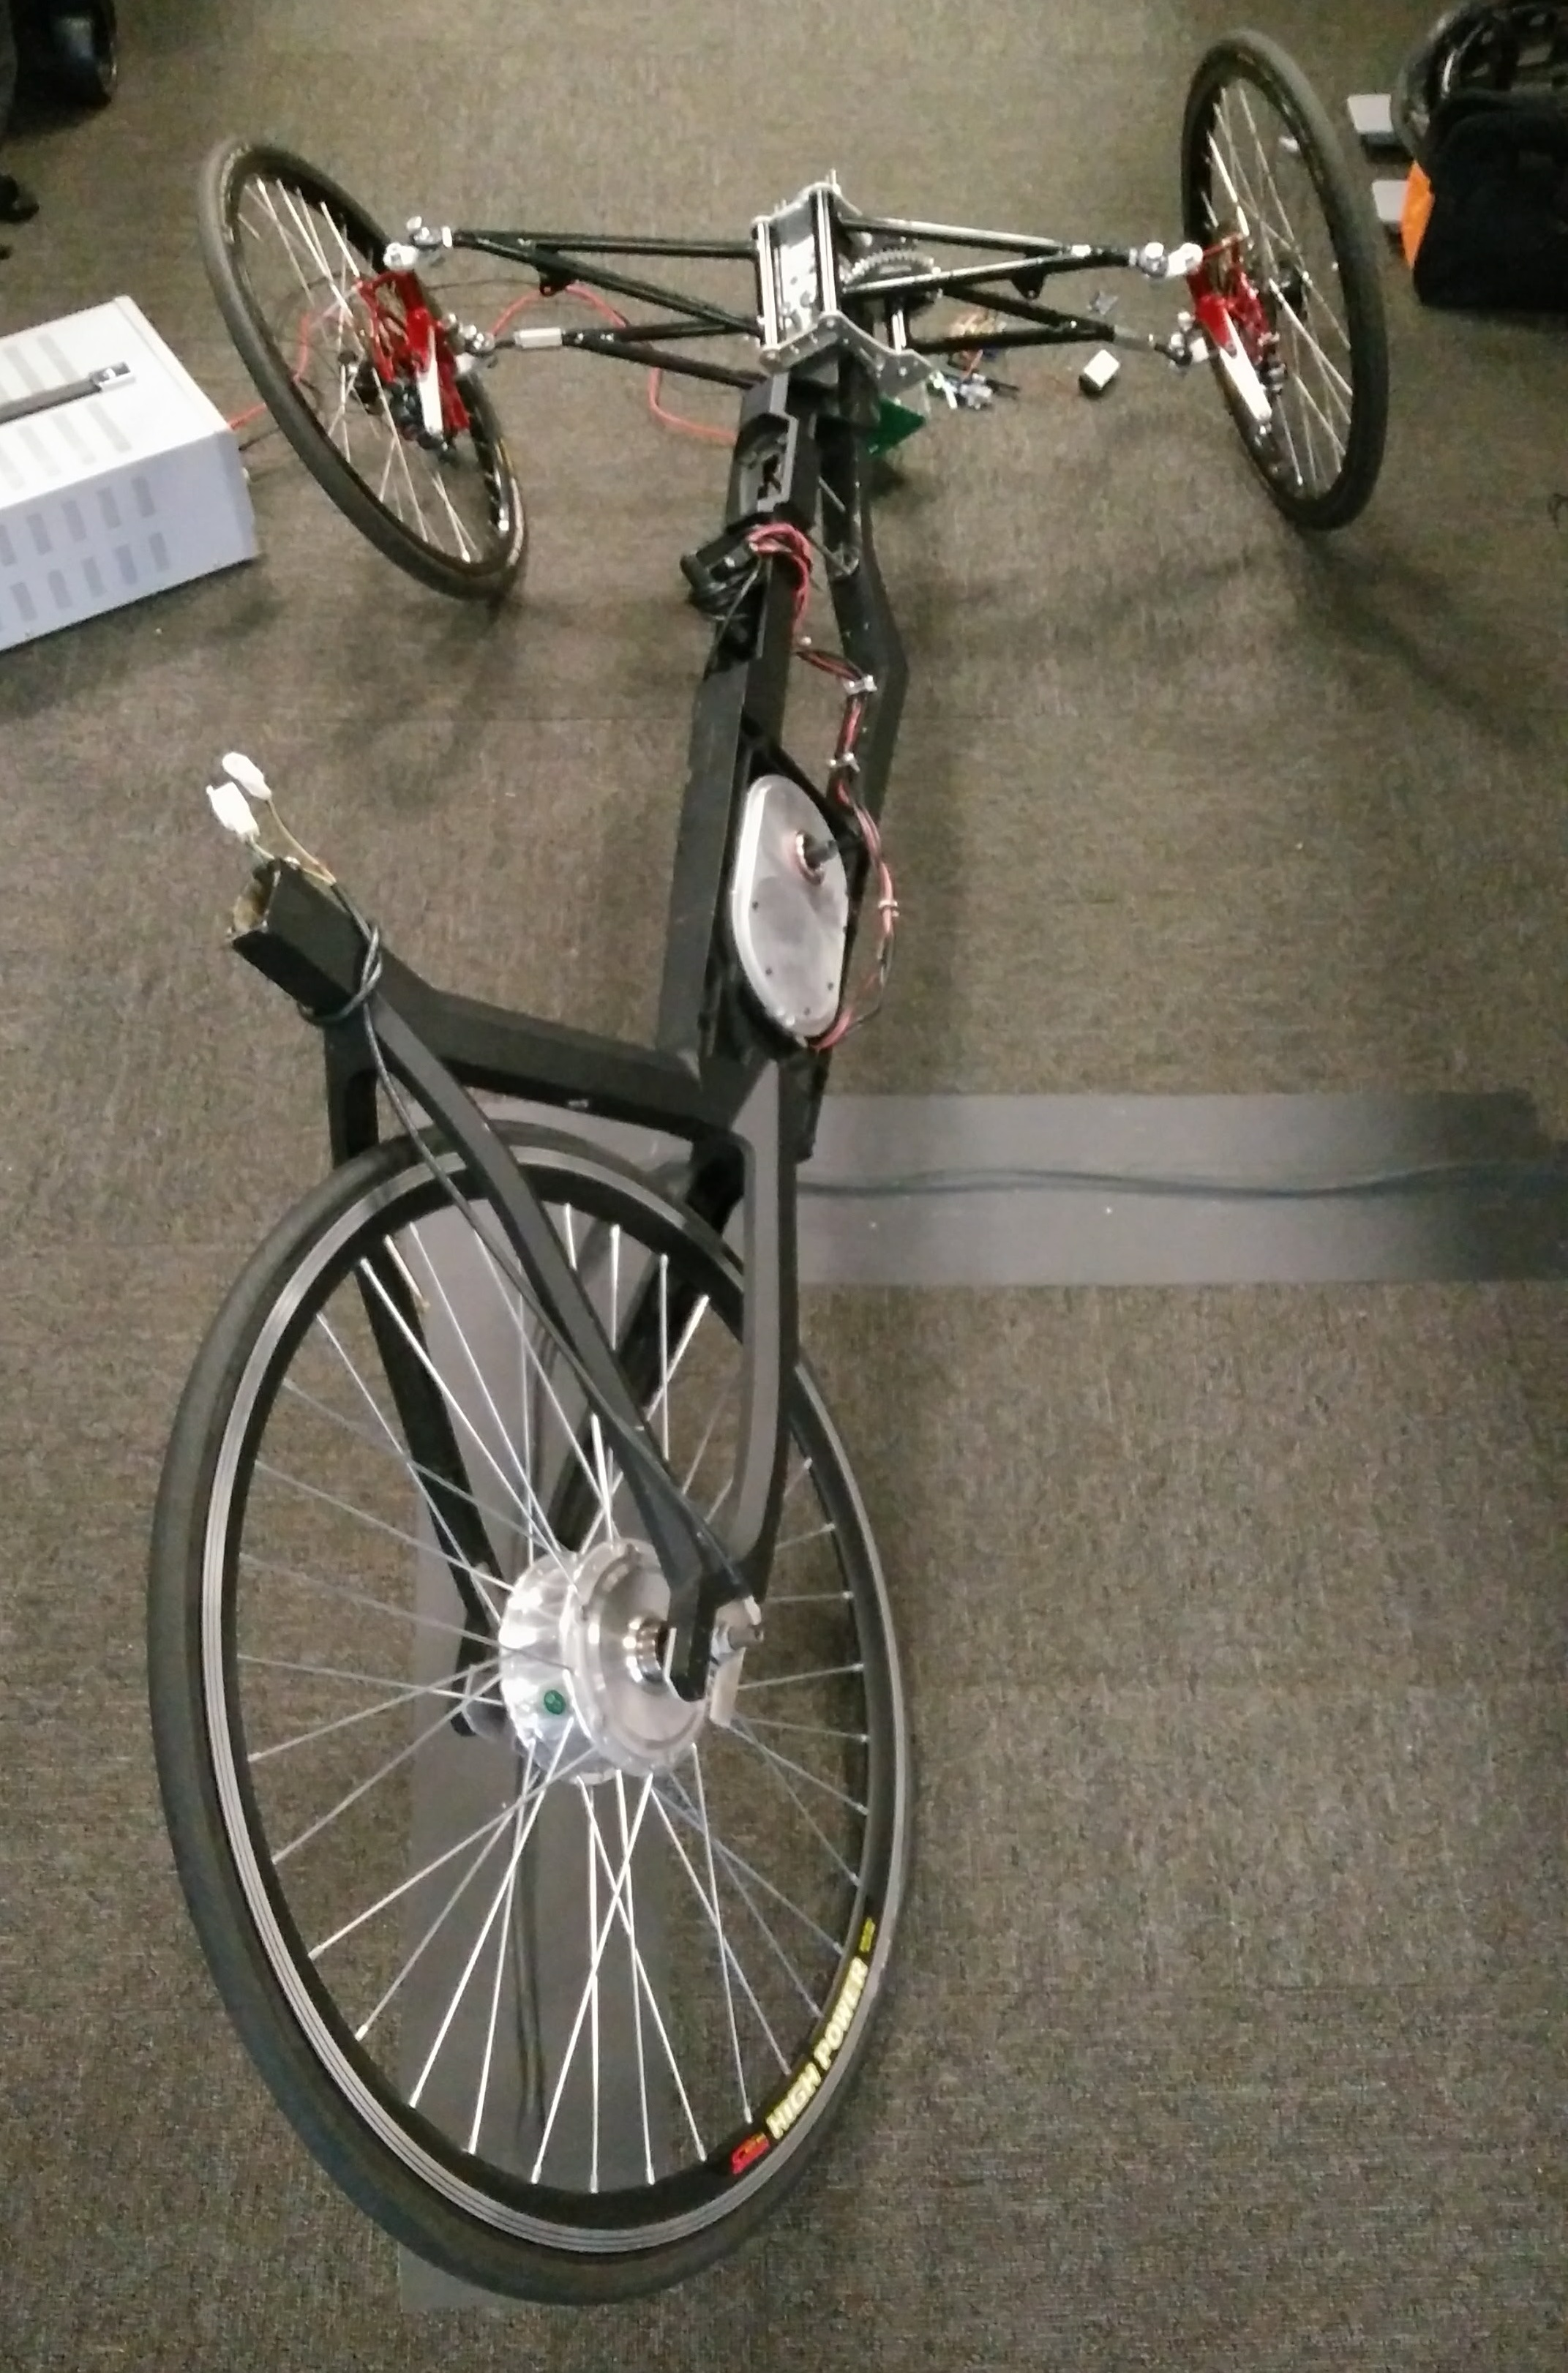
\includegraphics[width=0.95\linewidth]{figs/05/IMG_20161231_124145}
	\caption{Top view: PEV tilting, first test without steering }
\end{marginfigure}
\newpage

\begin{figure}[h!]
	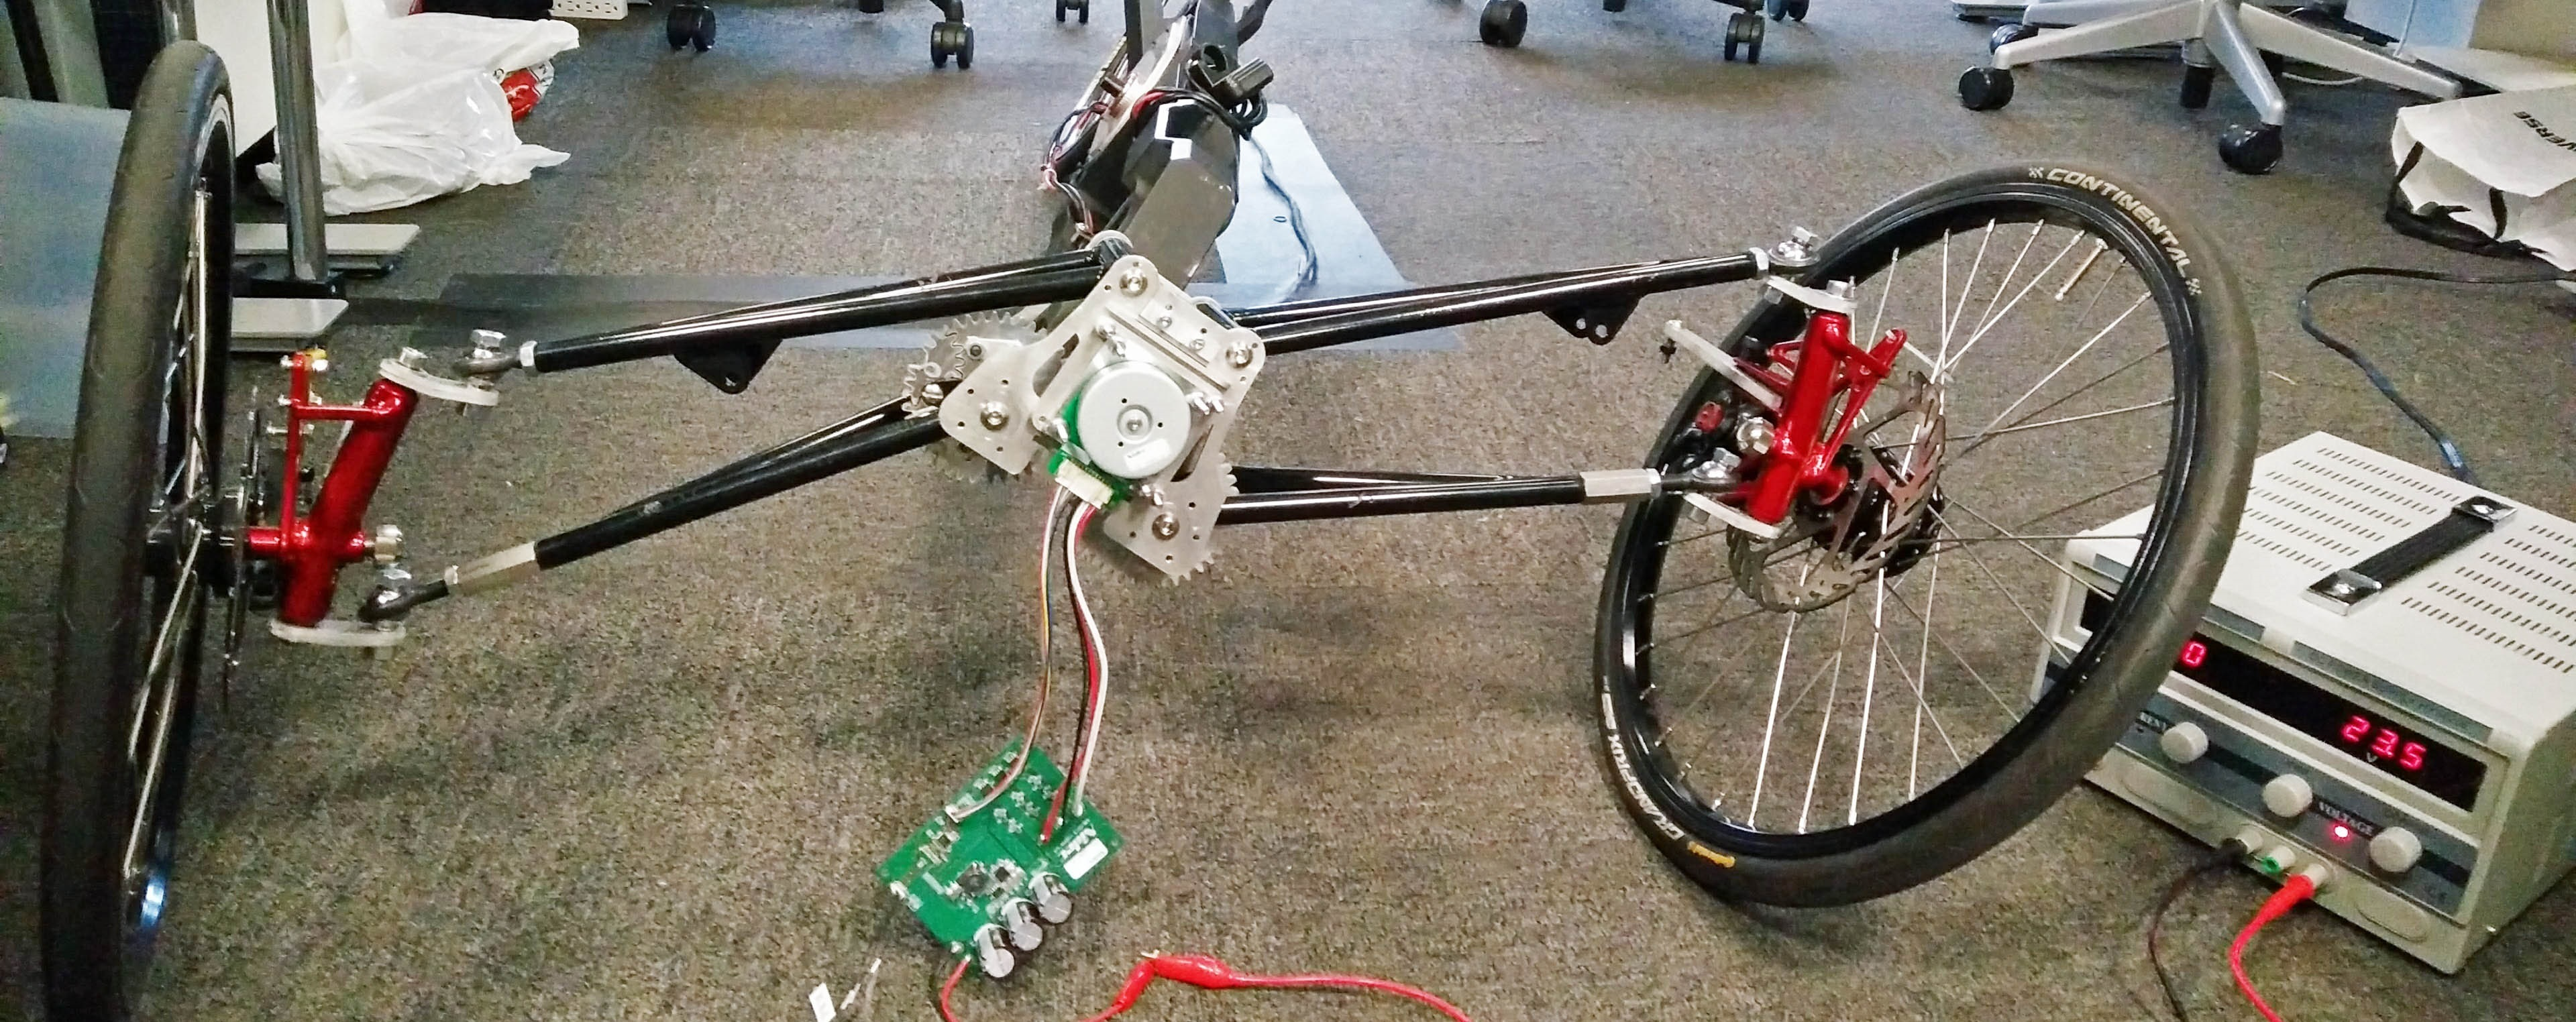
\includegraphics[width=0.95\linewidth]{figs/05/IMG_20161231_124120}
	\caption{Front view: PEV tilting, first test without steering}
	\\[-0.5cm]
\end{figure}
\begin{figure}[h!]
	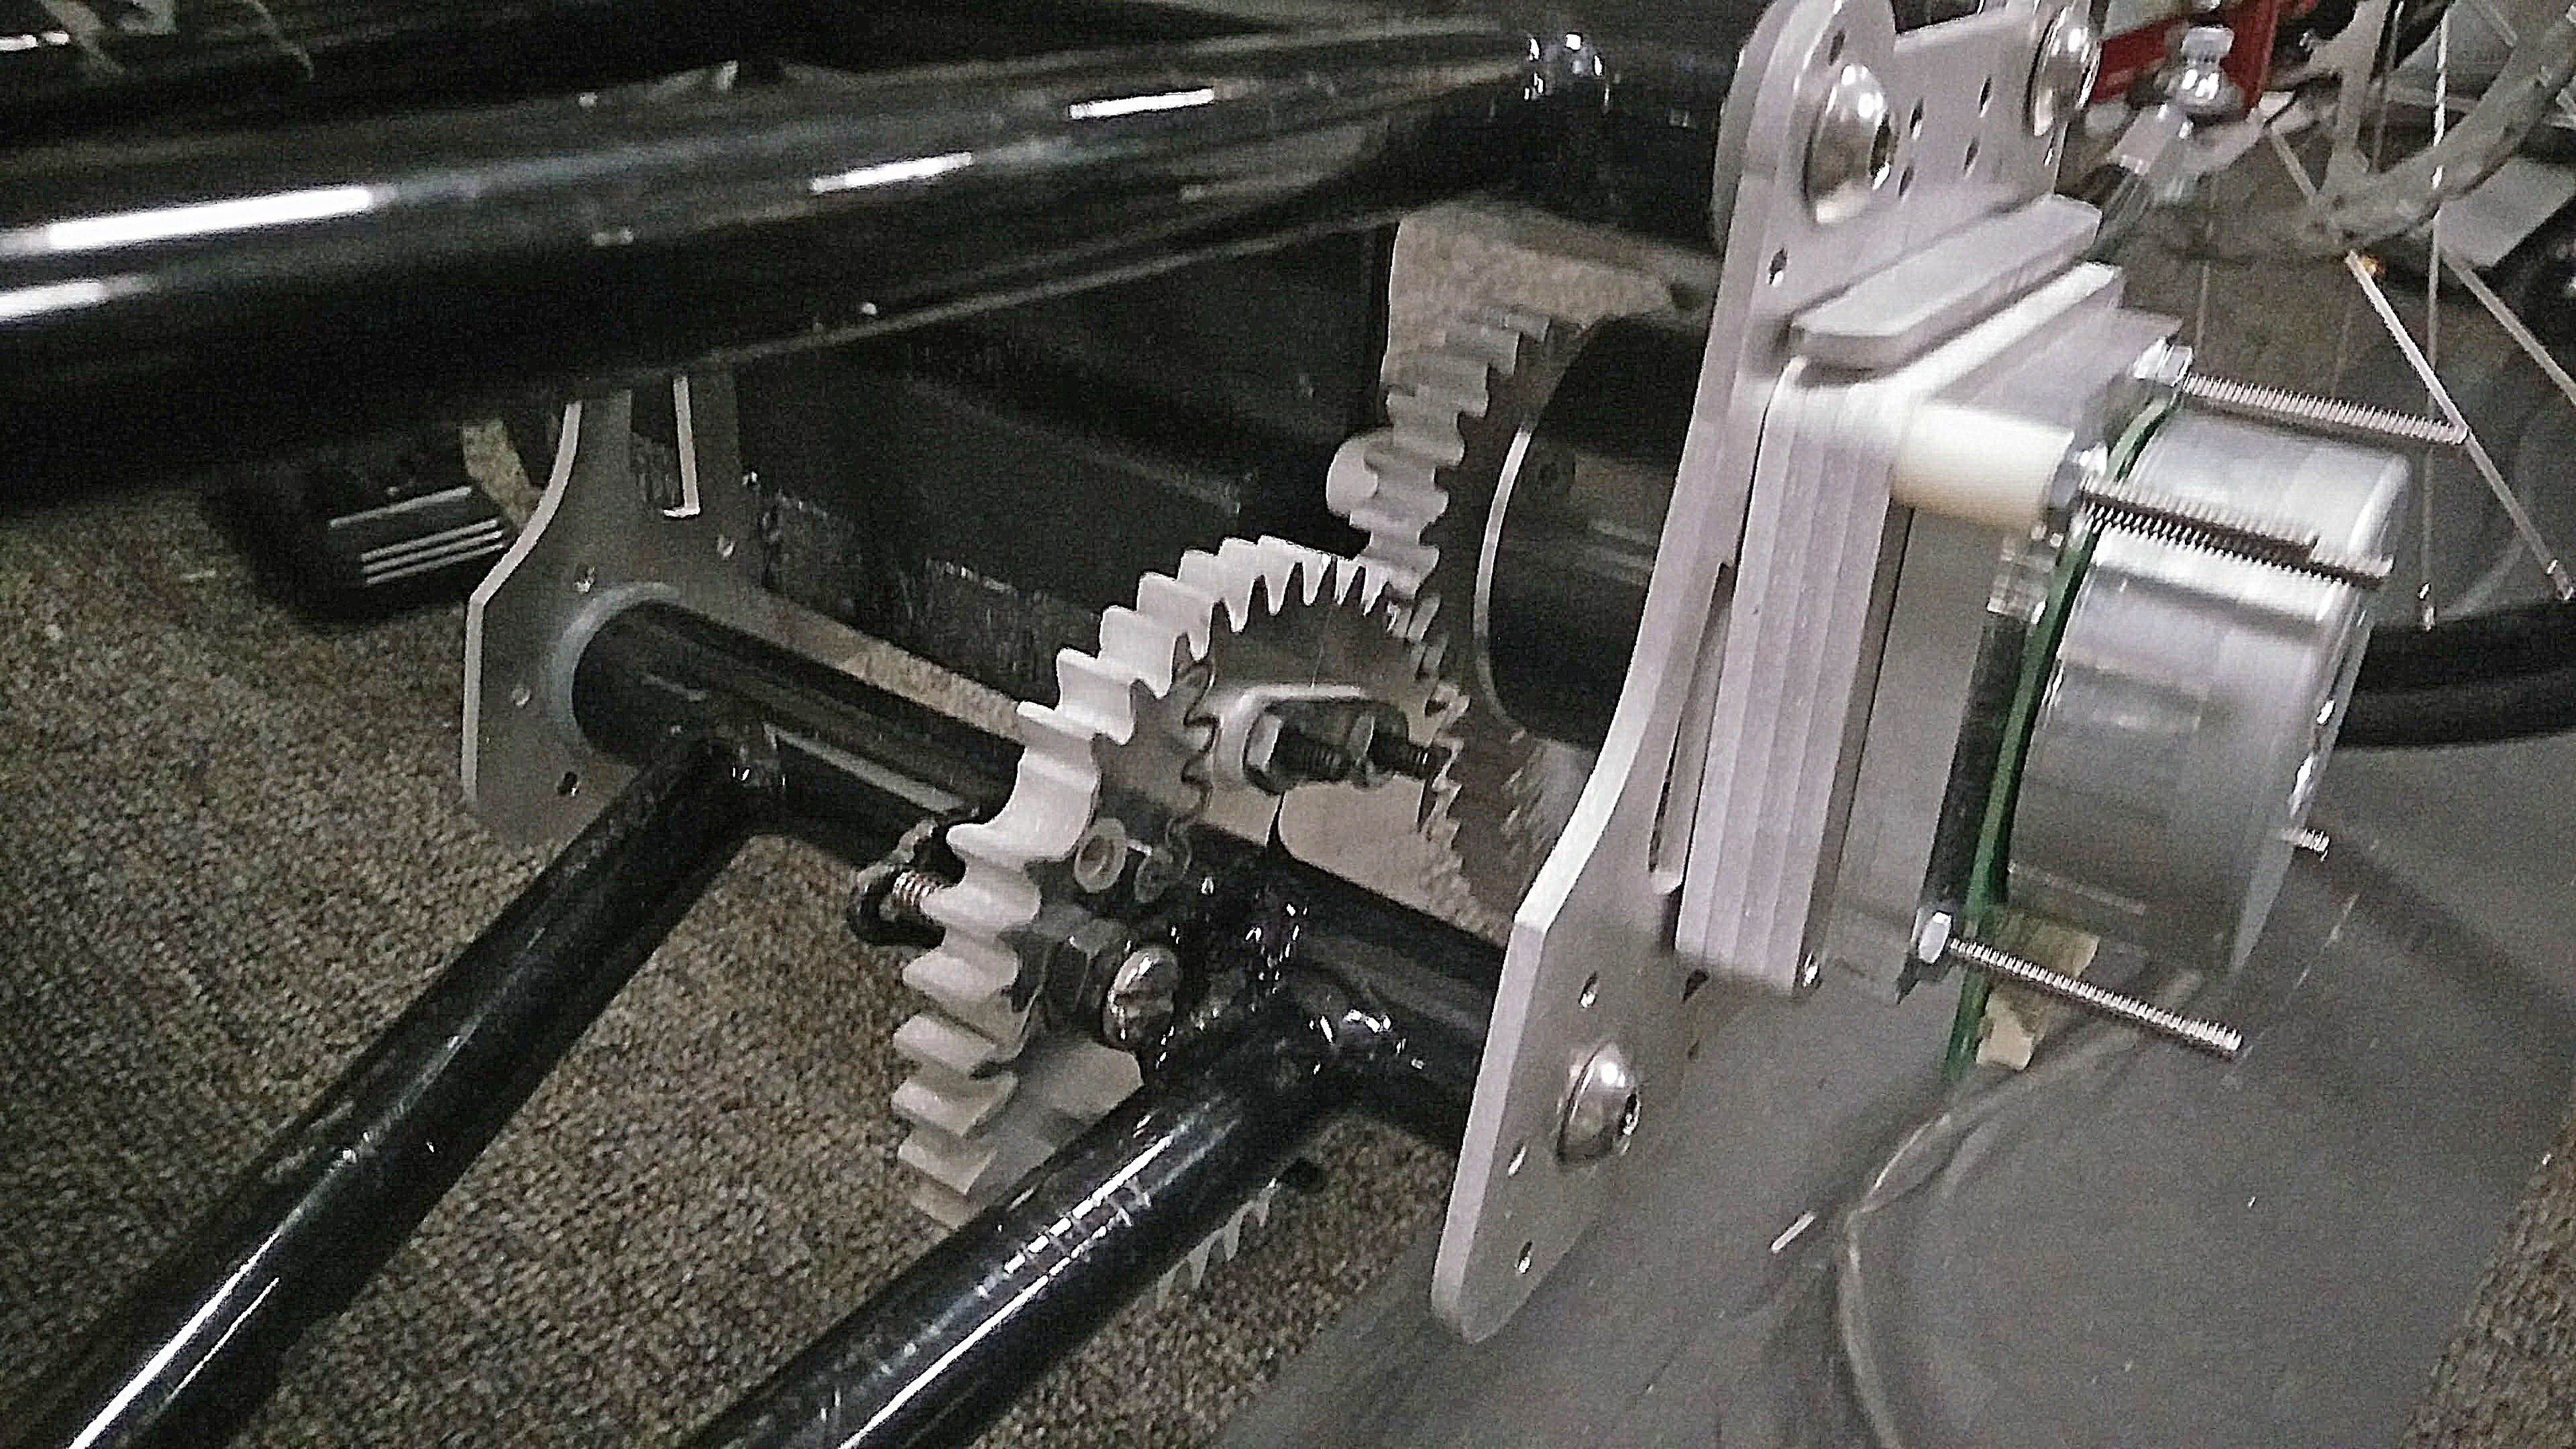
\includegraphics[width=0.95\linewidth]{figs/05/IMG_20161230_212159}
	\caption{Tilting mechanism: motor and gears}
	\\[-0.5cm]
\end{figure}
\begin{figure}[h!]
	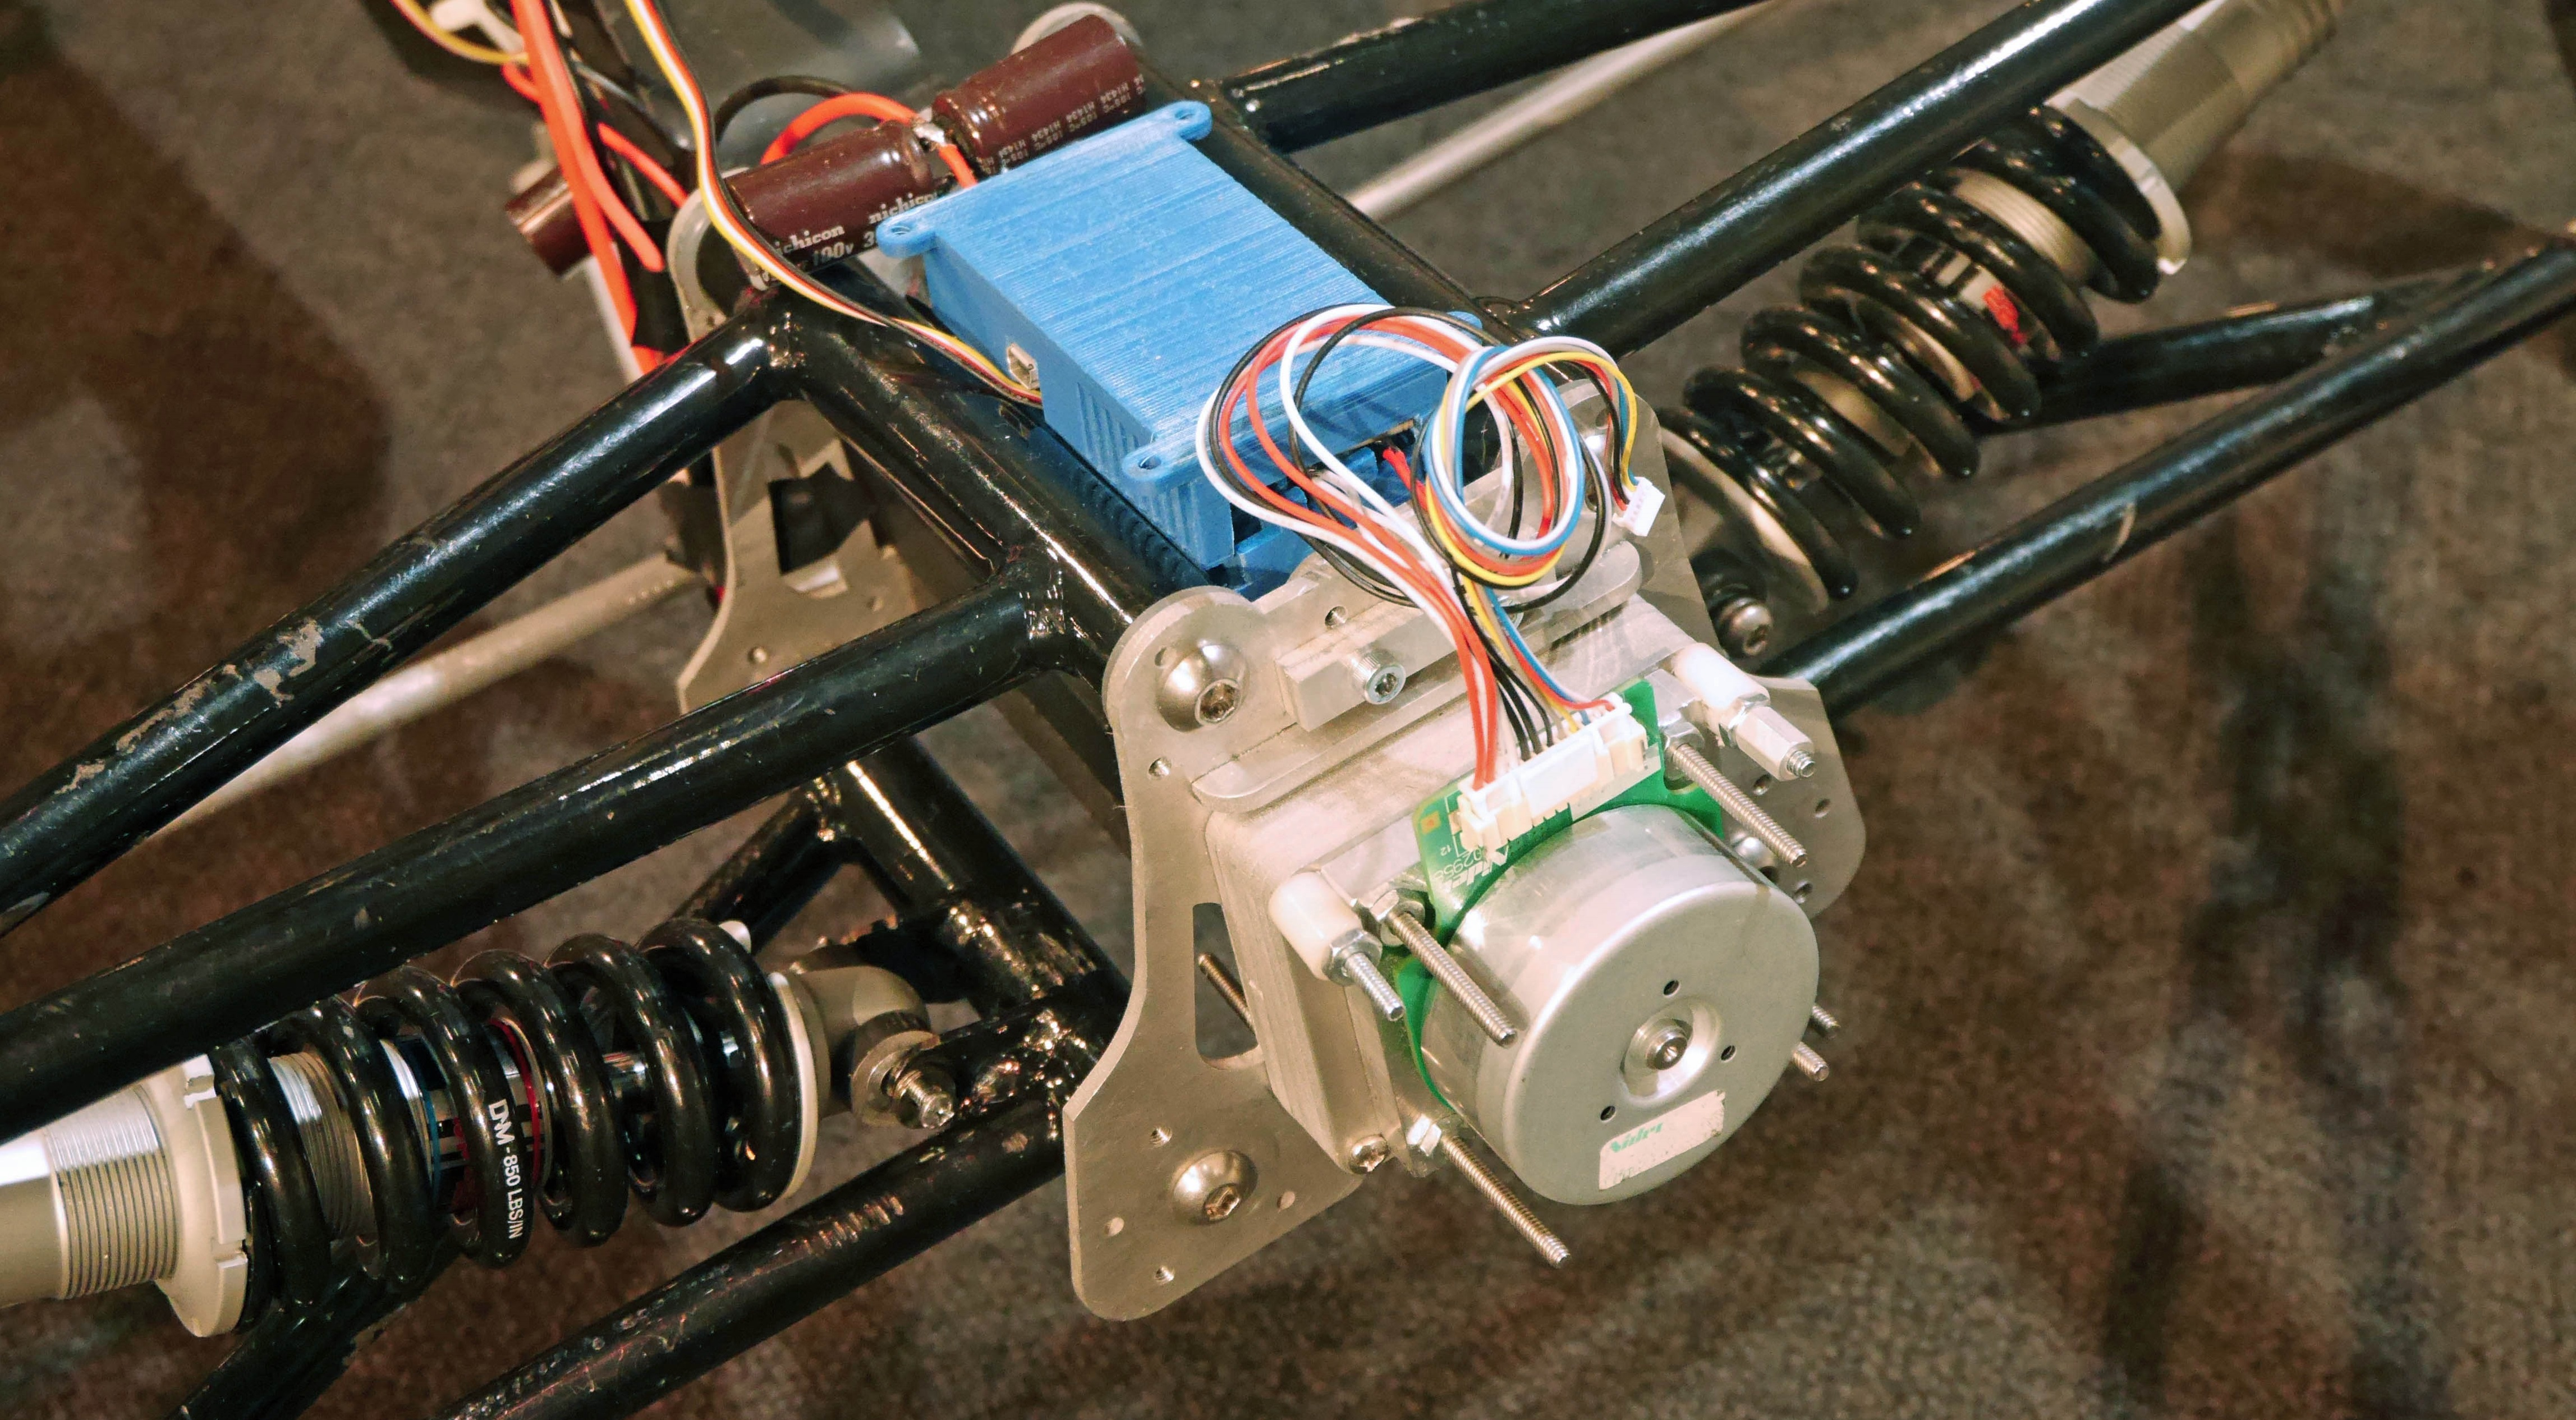
\includegraphics[width=0.95\linewidth]{figs/05/P1050722}
	\caption{Front suspension without tilting}
	\label{P1050722}
	\\[-0.5cm]
\end{figure}
\begin{figure}[h!]
	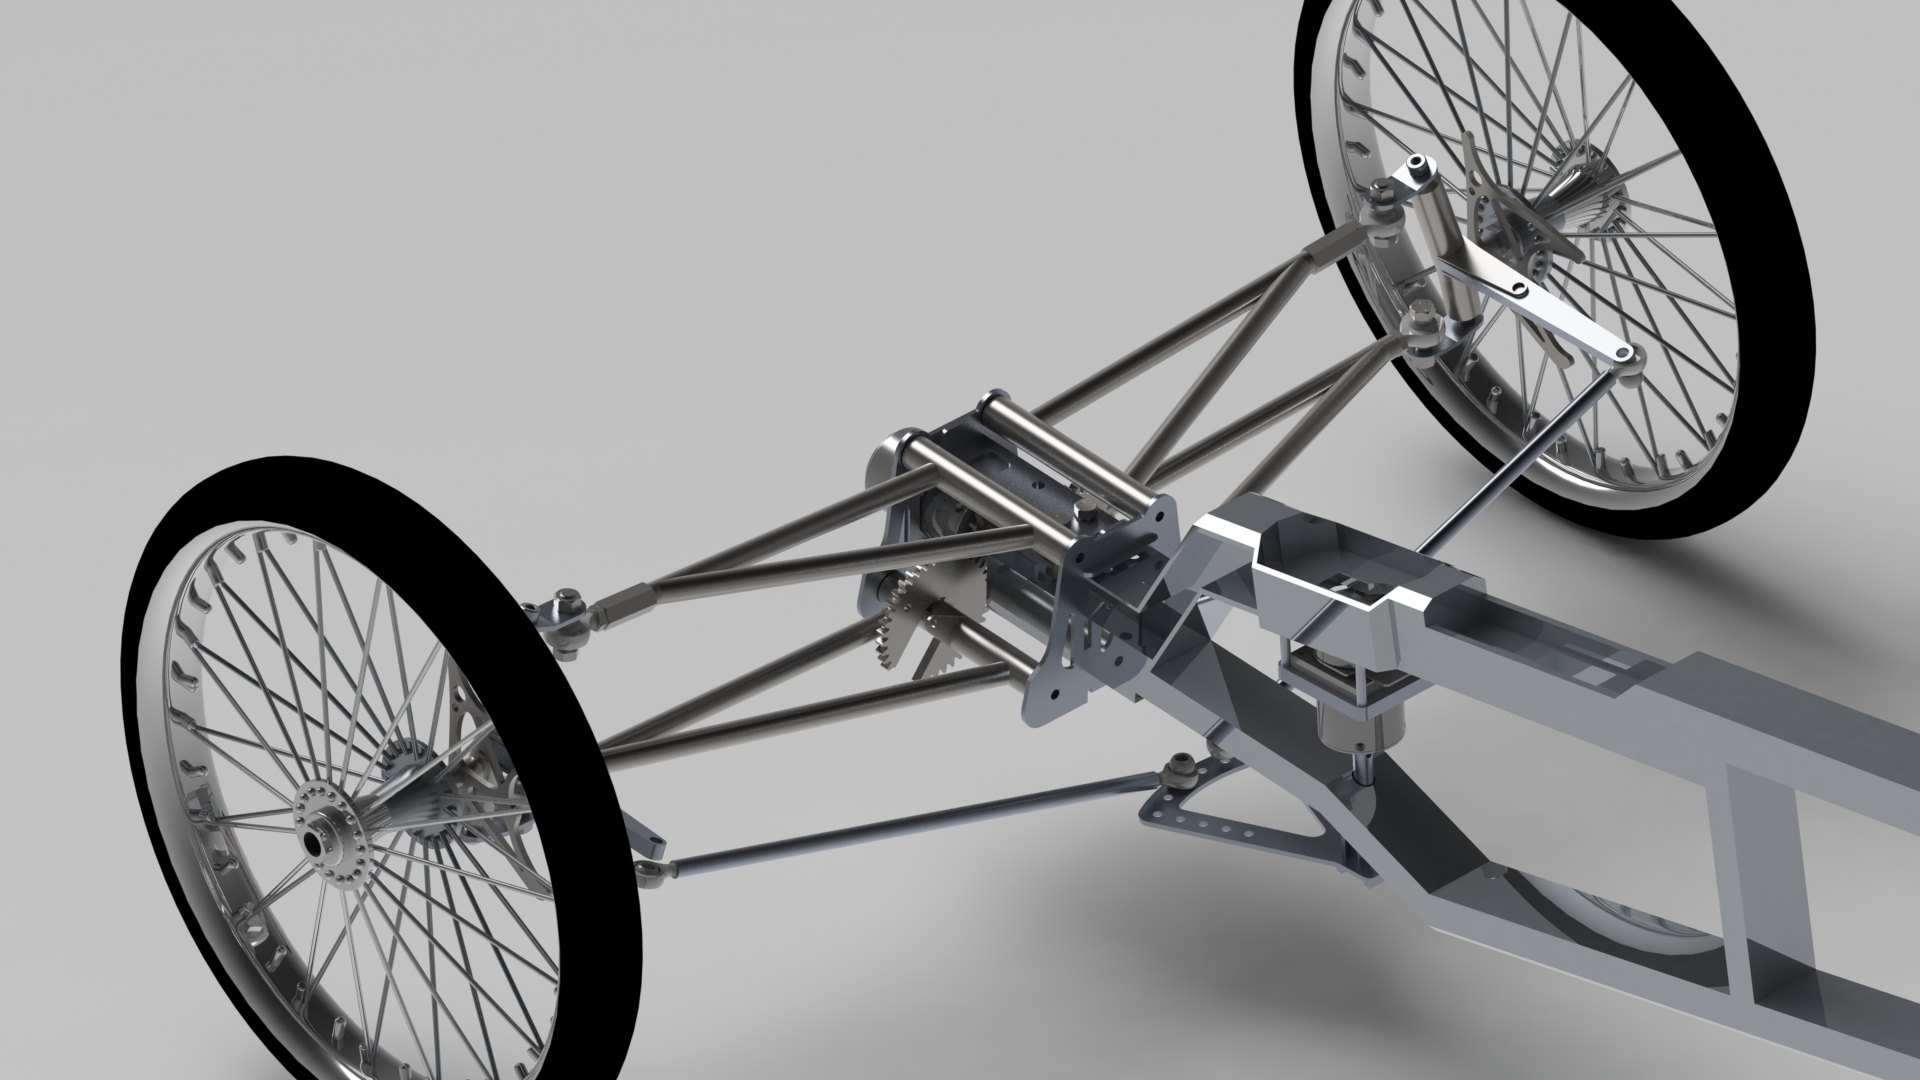
\includegraphics[width=0.95\linewidth]{figs/05/Render_Design_B_2}
	\caption{Render of the front suspension}
	\\[-1cm]
\end{figure}

\newpage

\subsection{Steering}
\begin{marginfigure}[2cm]
	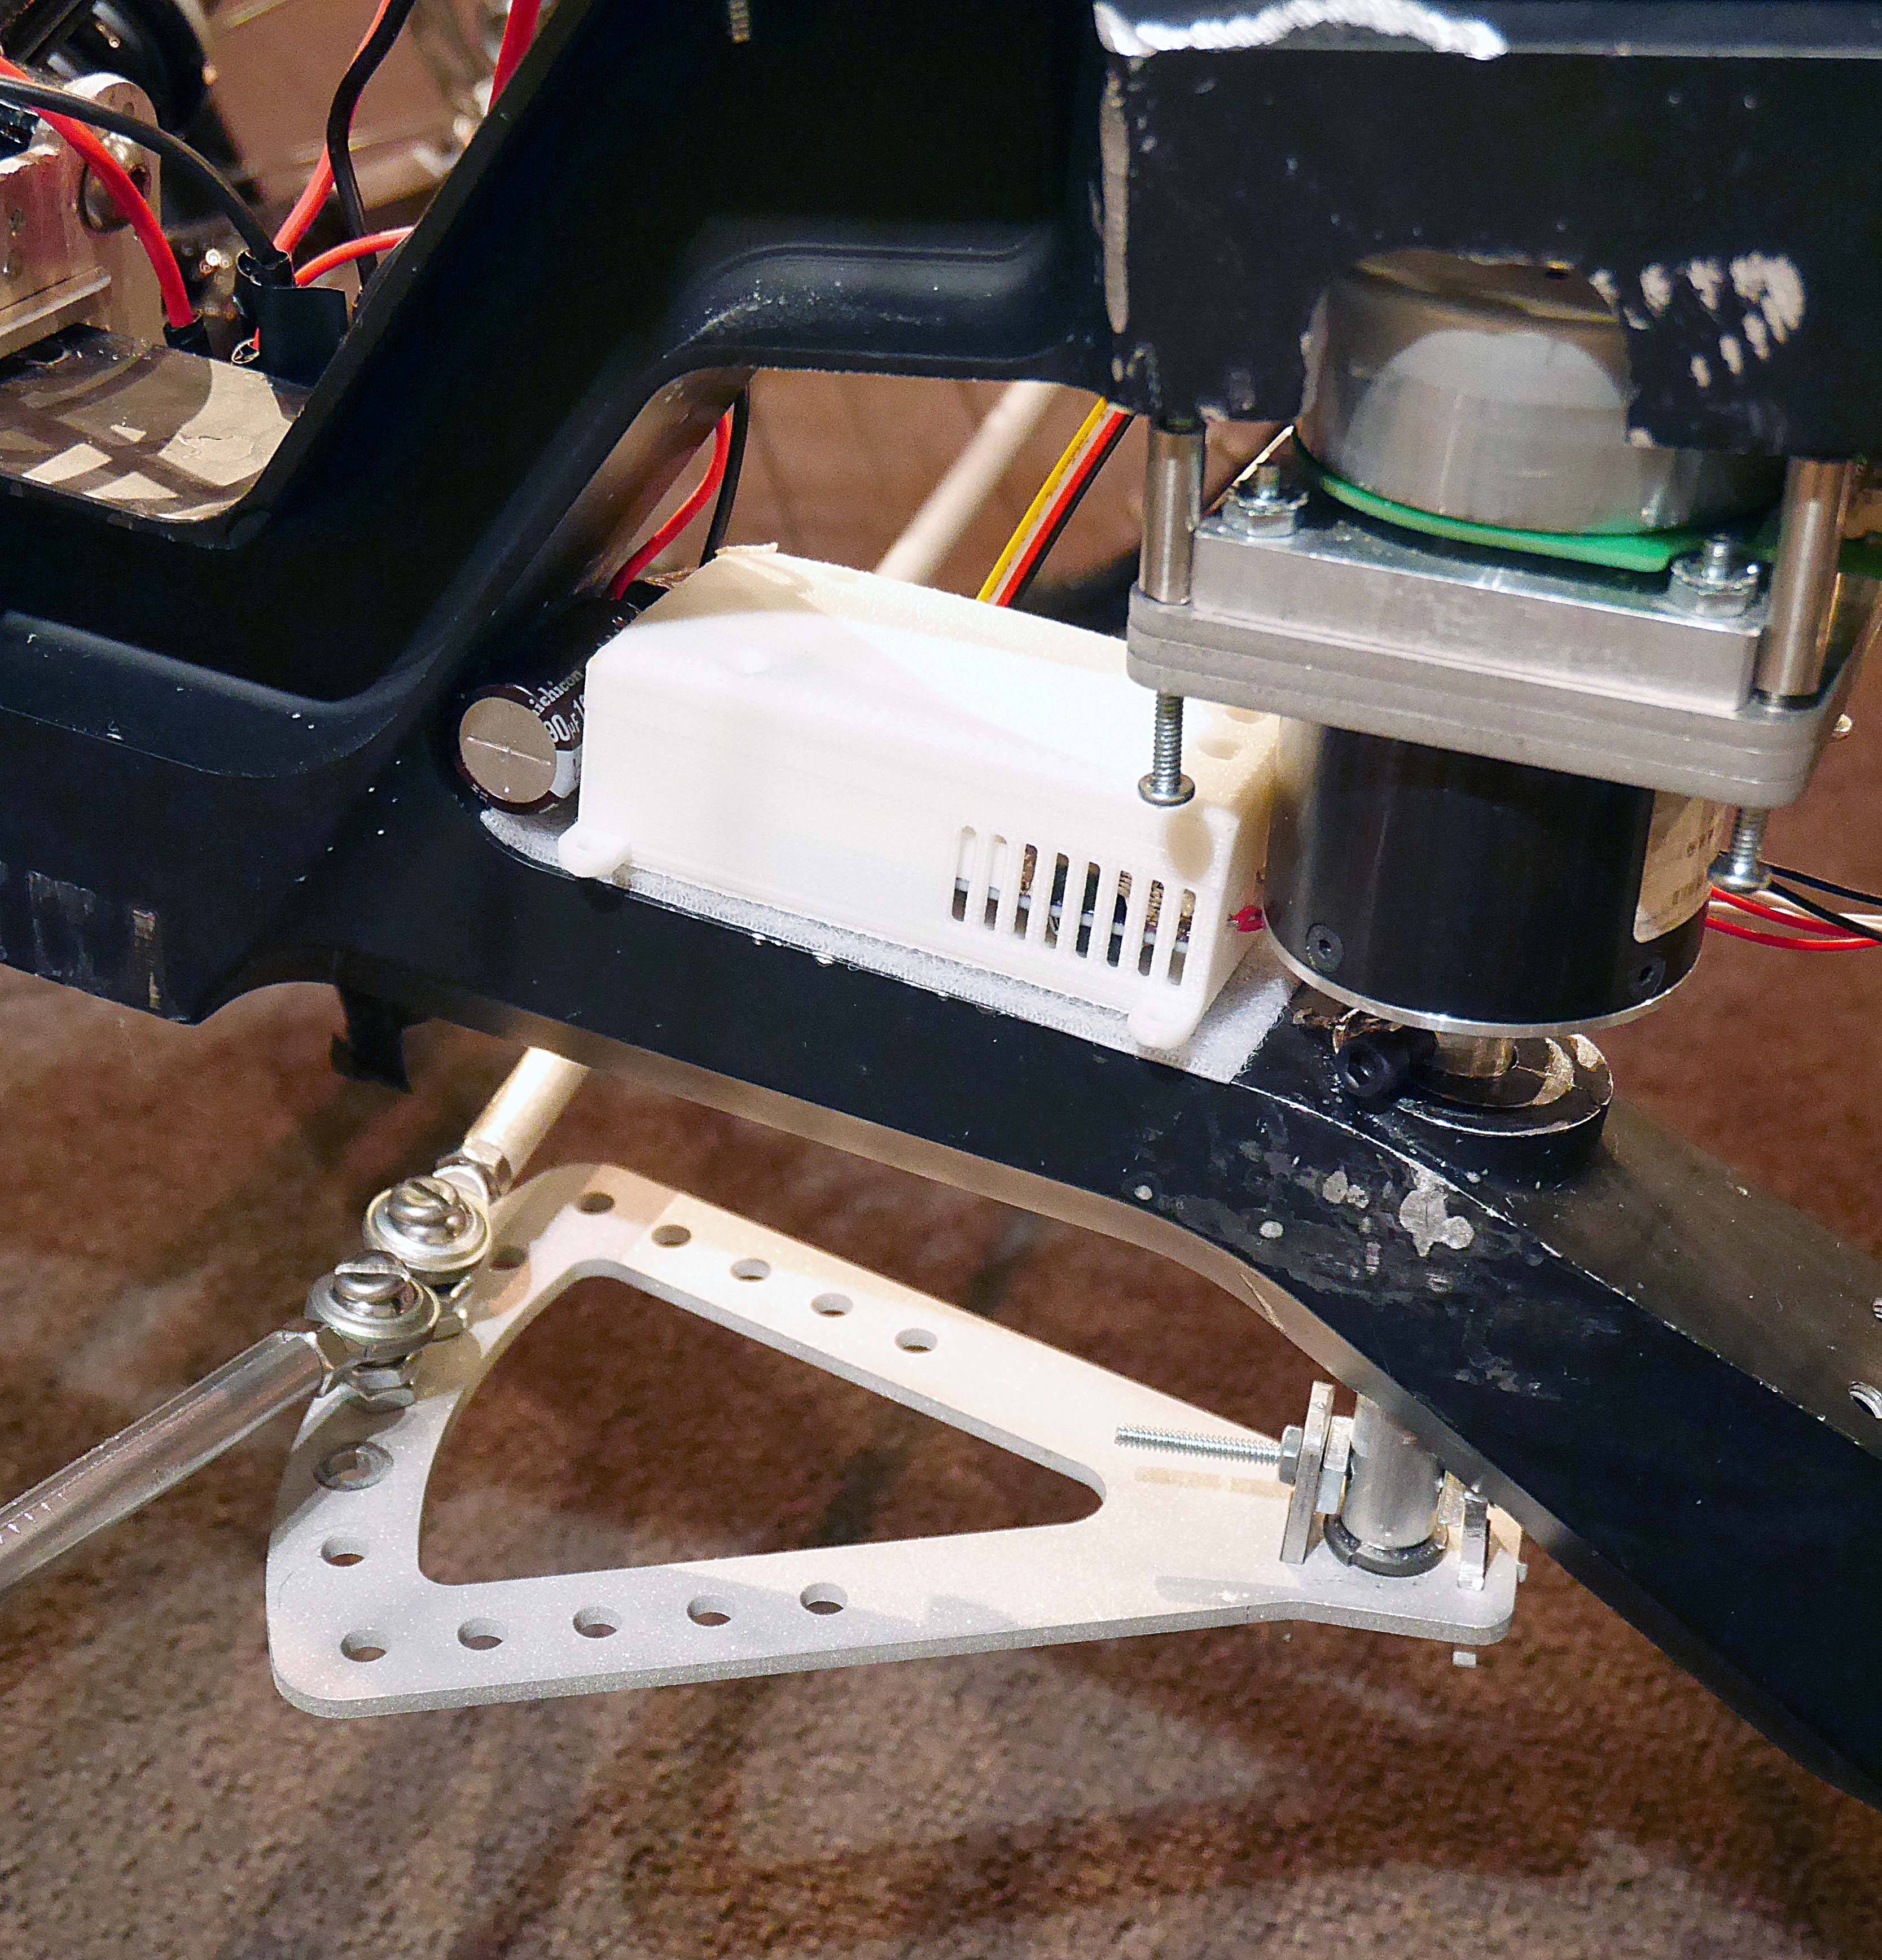
\includegraphics[width=1.1\linewidth]{figs/05/P1050723}
	\caption{Steering mechanism, NIDEC motor and VESC controller}
	\label{P1050723}
\end{marginfigure}

During the fabrication process it was decided to implement a steer-by-wire system. There were two main reasons to justify this system:
\begin{itemize}
\begin{itemize}
\item \textbf{SDTC}: by introducing a motor to control the steering mechanism, there is the possibility of changing the steer angle from the driver. The SDTC control strategy requires the control of the wheels to modify the path of the vehicle and tilt the vehicle by countersteering at high speeds. Even though in this project there was no time for implementing the SDTC, the steer-by-wire system remains useful for future applications of this vehicle.

\item \textbf{Autonomy}: an actuated steering system is a basic feature for an autonomous lightweight vehicle. If a fleet of PEV is on the streets and a user calls one of them, it will need of a motorized propulsion and steering as well. In a reduced manner, in this project it was possible to remotely control the PEV and test it without a driver.
\end{itemize}
\end{itemize}

The main drawback of the steer-by-wire system is that it requires to be constantly powered by the batteries. When the vehicle is powered off, the steering motor remains in the same position, until is powered again and the handle bar and the wheels align. 

Arduino boards do not have save any data after they are powered off. This fact implies that if the handle bar is moved during a no-power period, there will be a misalignment between the wheels and the handle bar. To avoid this problem, the absolute orientation of the IMU is used. By configuring the IMU properly, the orientation with respect to an inertial frame can be obtained. In case that the vehicle is rotated, there will also be a misalignment again, so two identical IMUs were necessary. The relative angle between them will report to the motor the initial angle of the wheels.
 
In the Figure \ref{P1050723}, the position of the motor and the steering mechanism is represented. Some modifications were made to the aluminum frame to allocate the motor. The output shaft goes through the frame, connected to another aluminum part. This part (Figure \ref{IMG_20170403_011512}) had several holes to adapt to the rest of attachments. The white case was 3D printed and contains the VESC controller.

\begin{figure}[h!]
	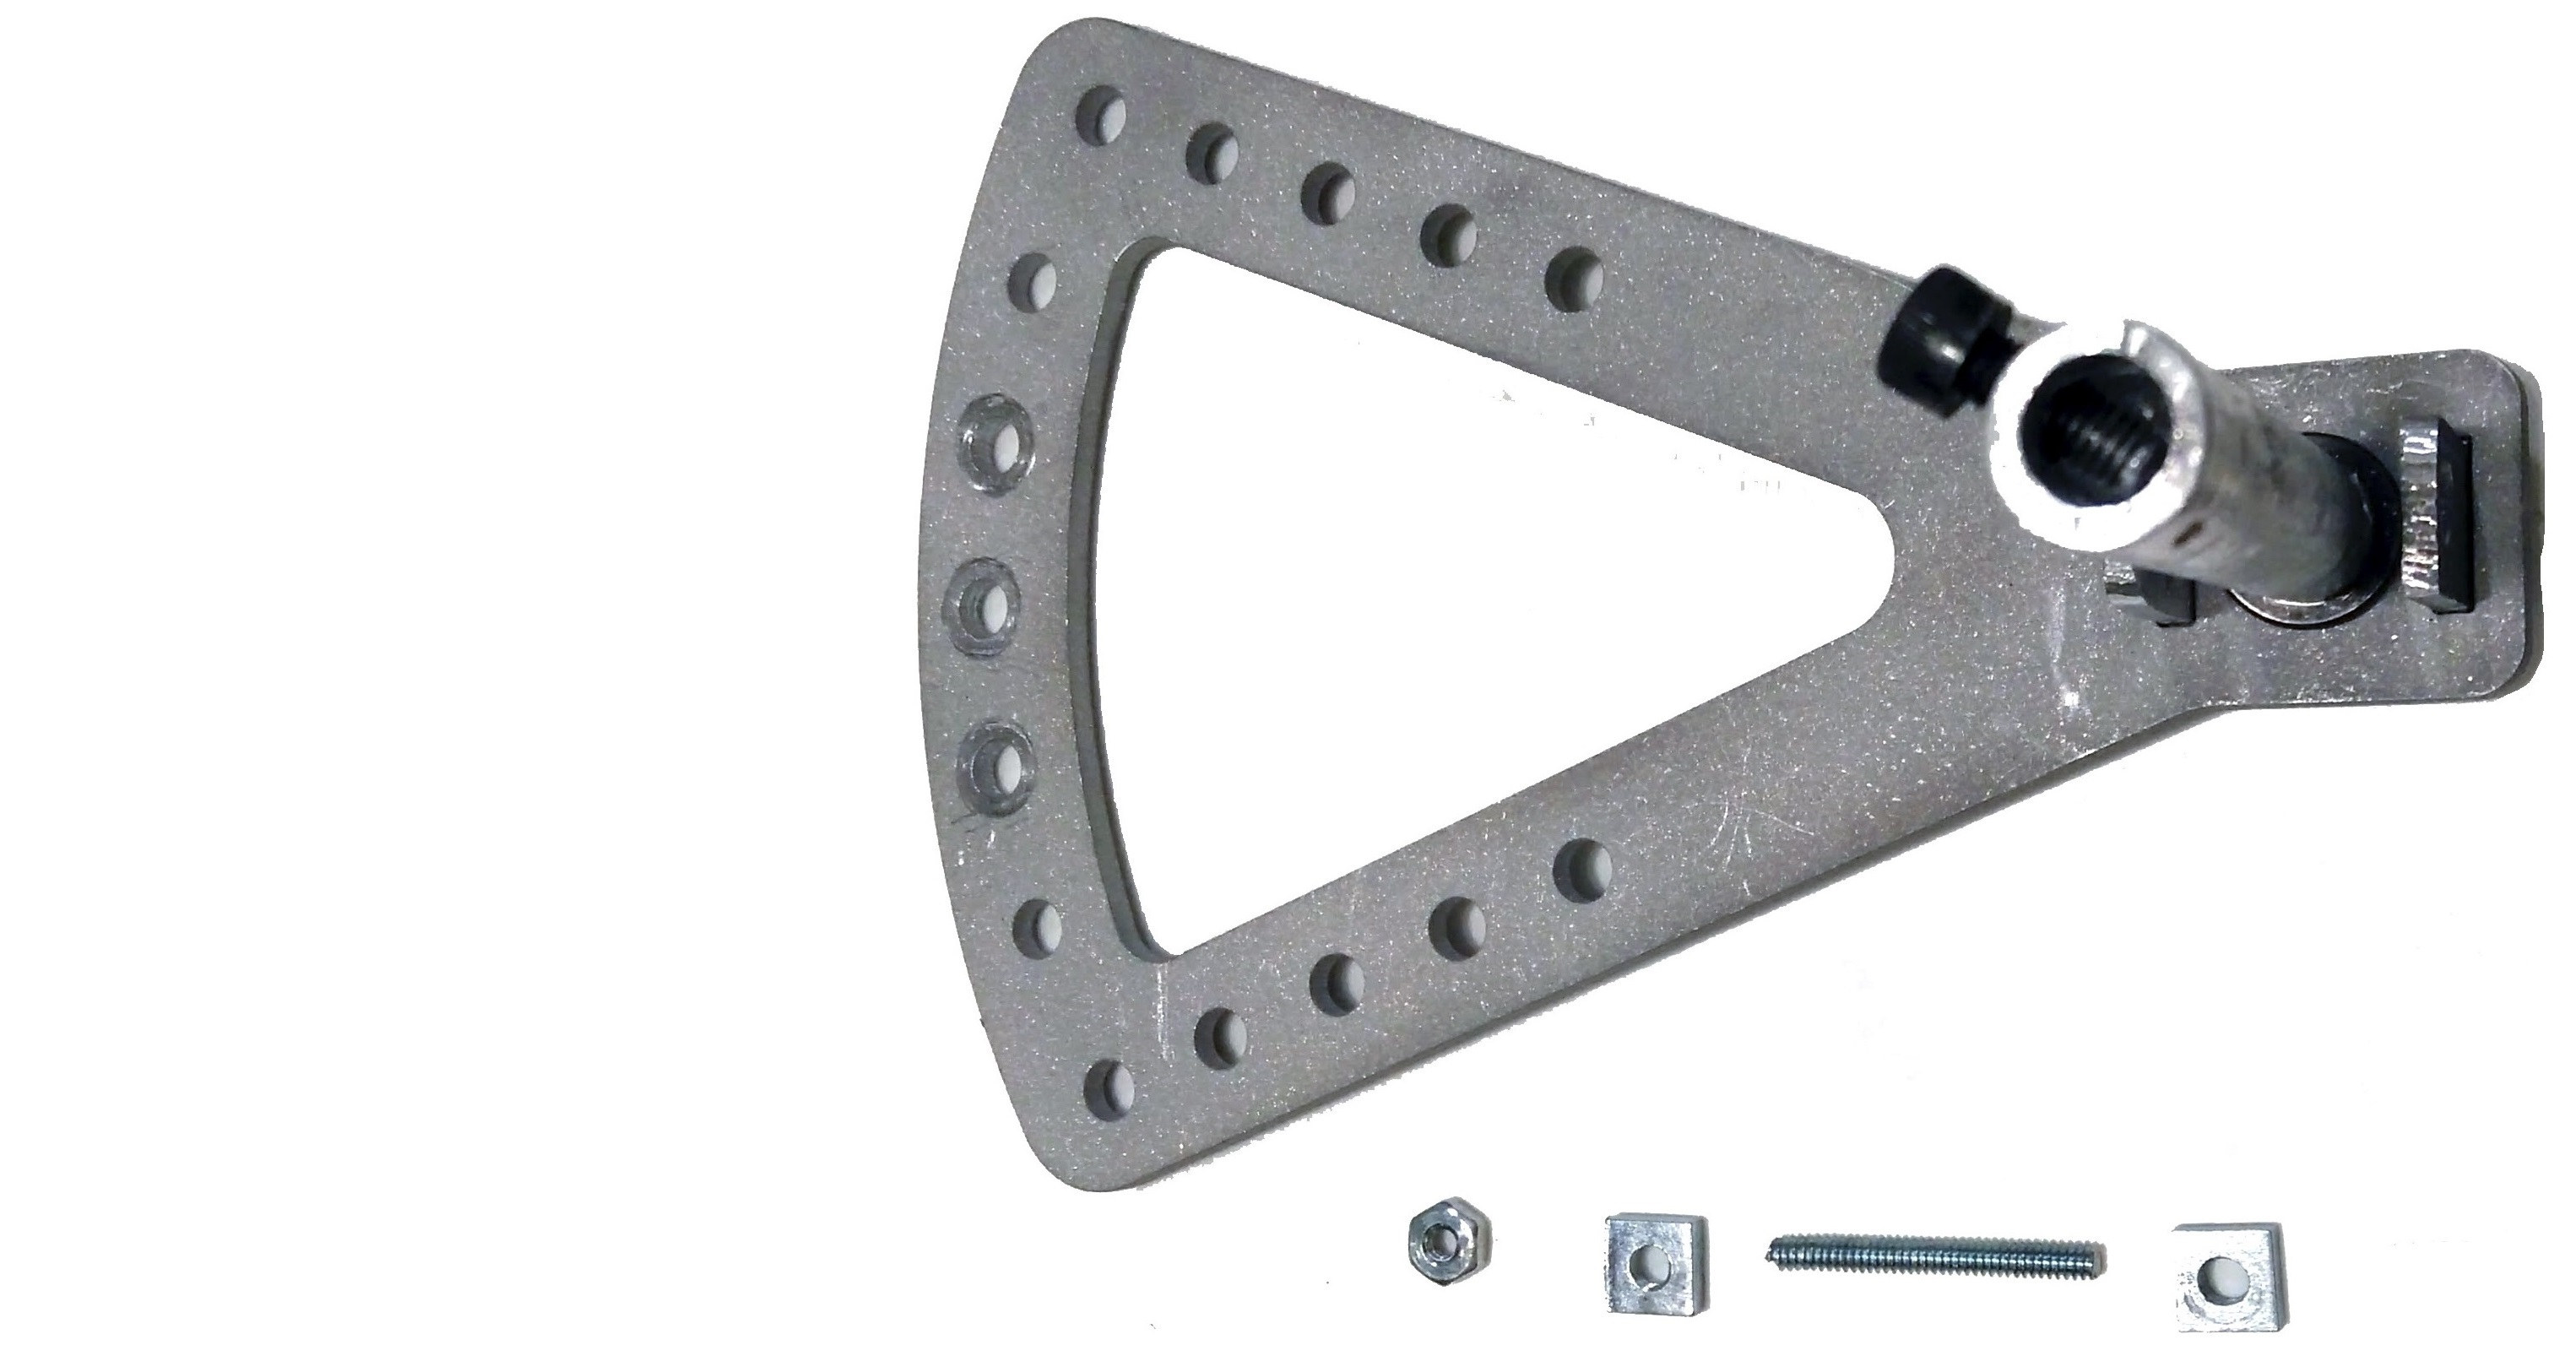
\includegraphics[width=0.7\linewidth]{figs/05/IMG_20170403_011512}
	\caption{Steering parts}
	\label{IMG_20170403_011512}
	\\[-5cm]
\end{figure}

\newpage
\subsection{Handle Bar}

Before approaching the design of the handle bar, it was necessary to build a column that supported it. The frame did not have any prepared holes or location for the steering column, so everything had to be designed from scratch and adapted to assure a good joining between the frame and the steering column.

\begin{figure}[h!]
	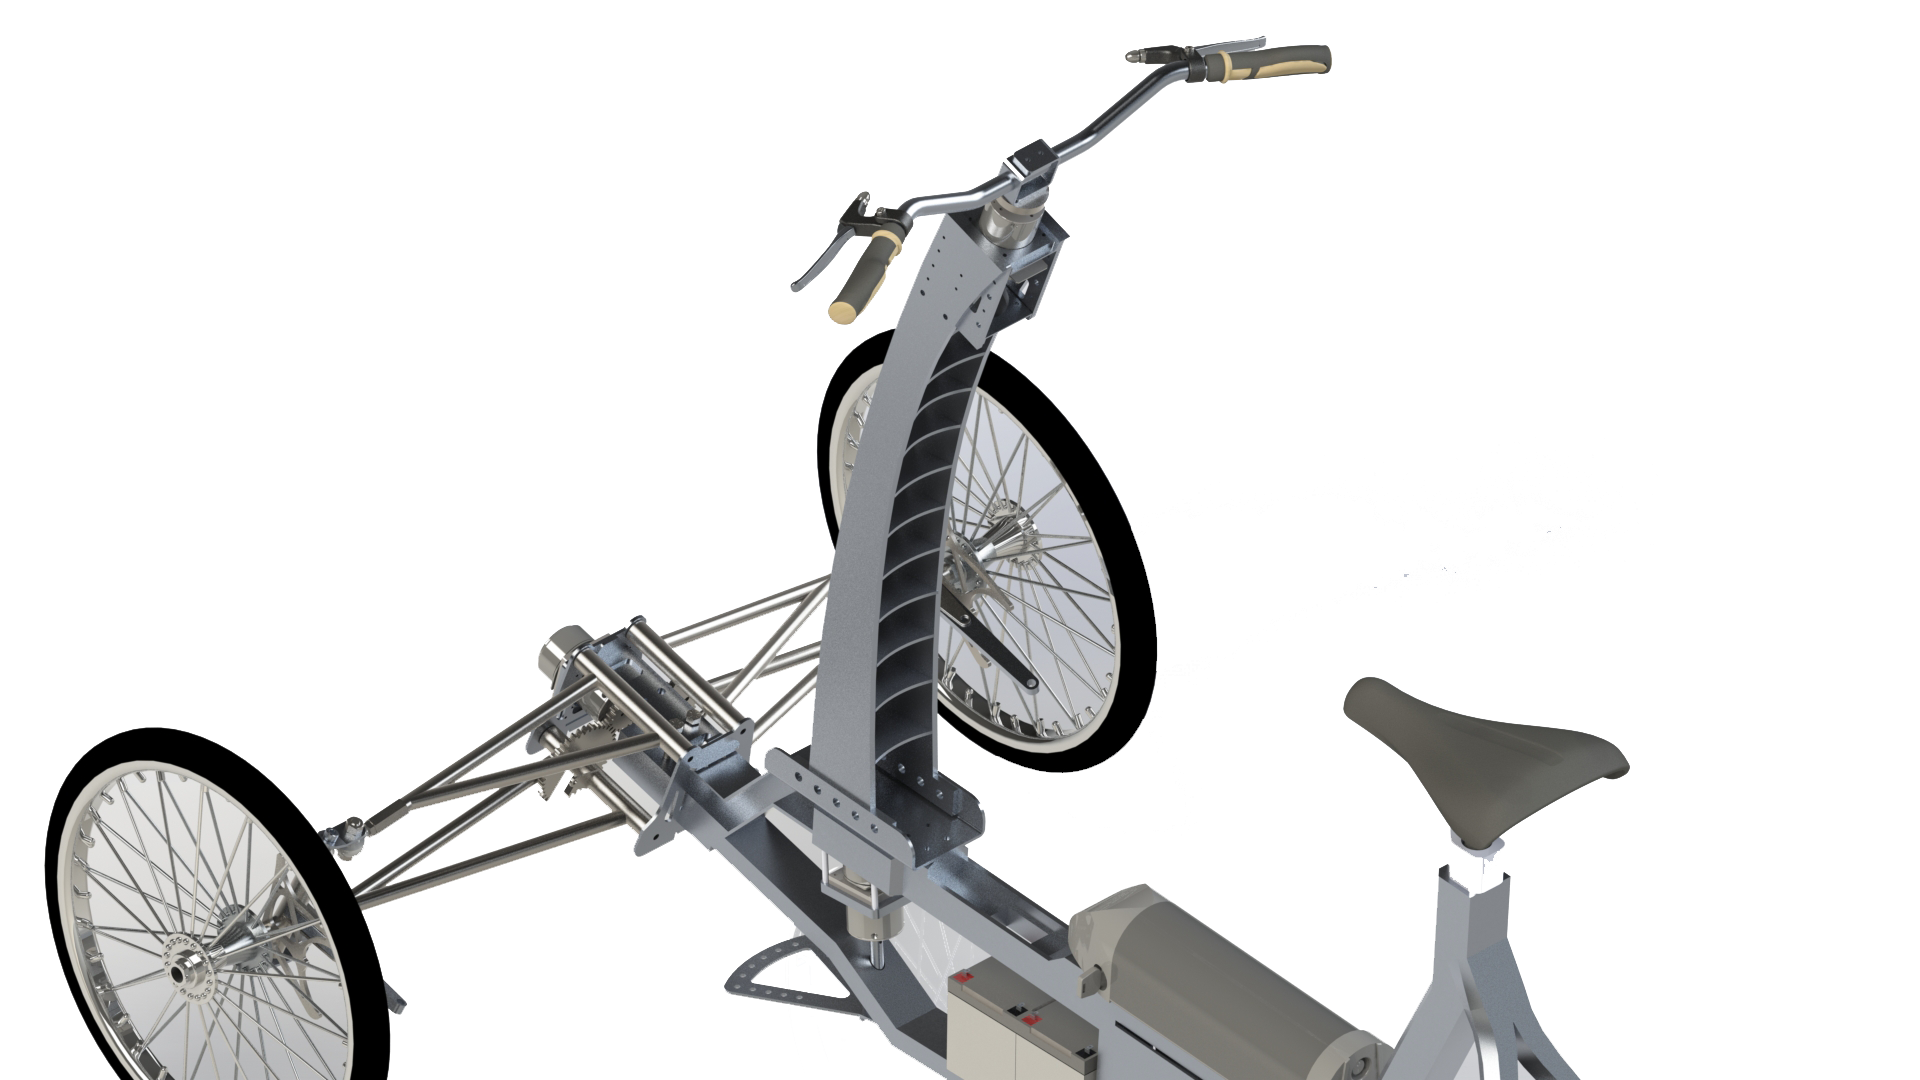
\includegraphics[width=1\linewidth]{figs/05/Render_Design_B_7}
	\caption{Handle bar and steering column render}
	\\[-1cm]
\end{figure}

The steer-by-wire system allowed a free design of the column, formed by two lateral aluminum sheets connected by thinner transversal sheets. These parts were water jetted, so a distinctive shape was selected for them. While the fabrication resulted really fast and easy, assembling all these parts required some time. The assembly was really tedious, requiring some clamps to put all the parts together (Figure \ref{IMG_20170207_154911}).

\begin{marginfigure}[-3cm]
	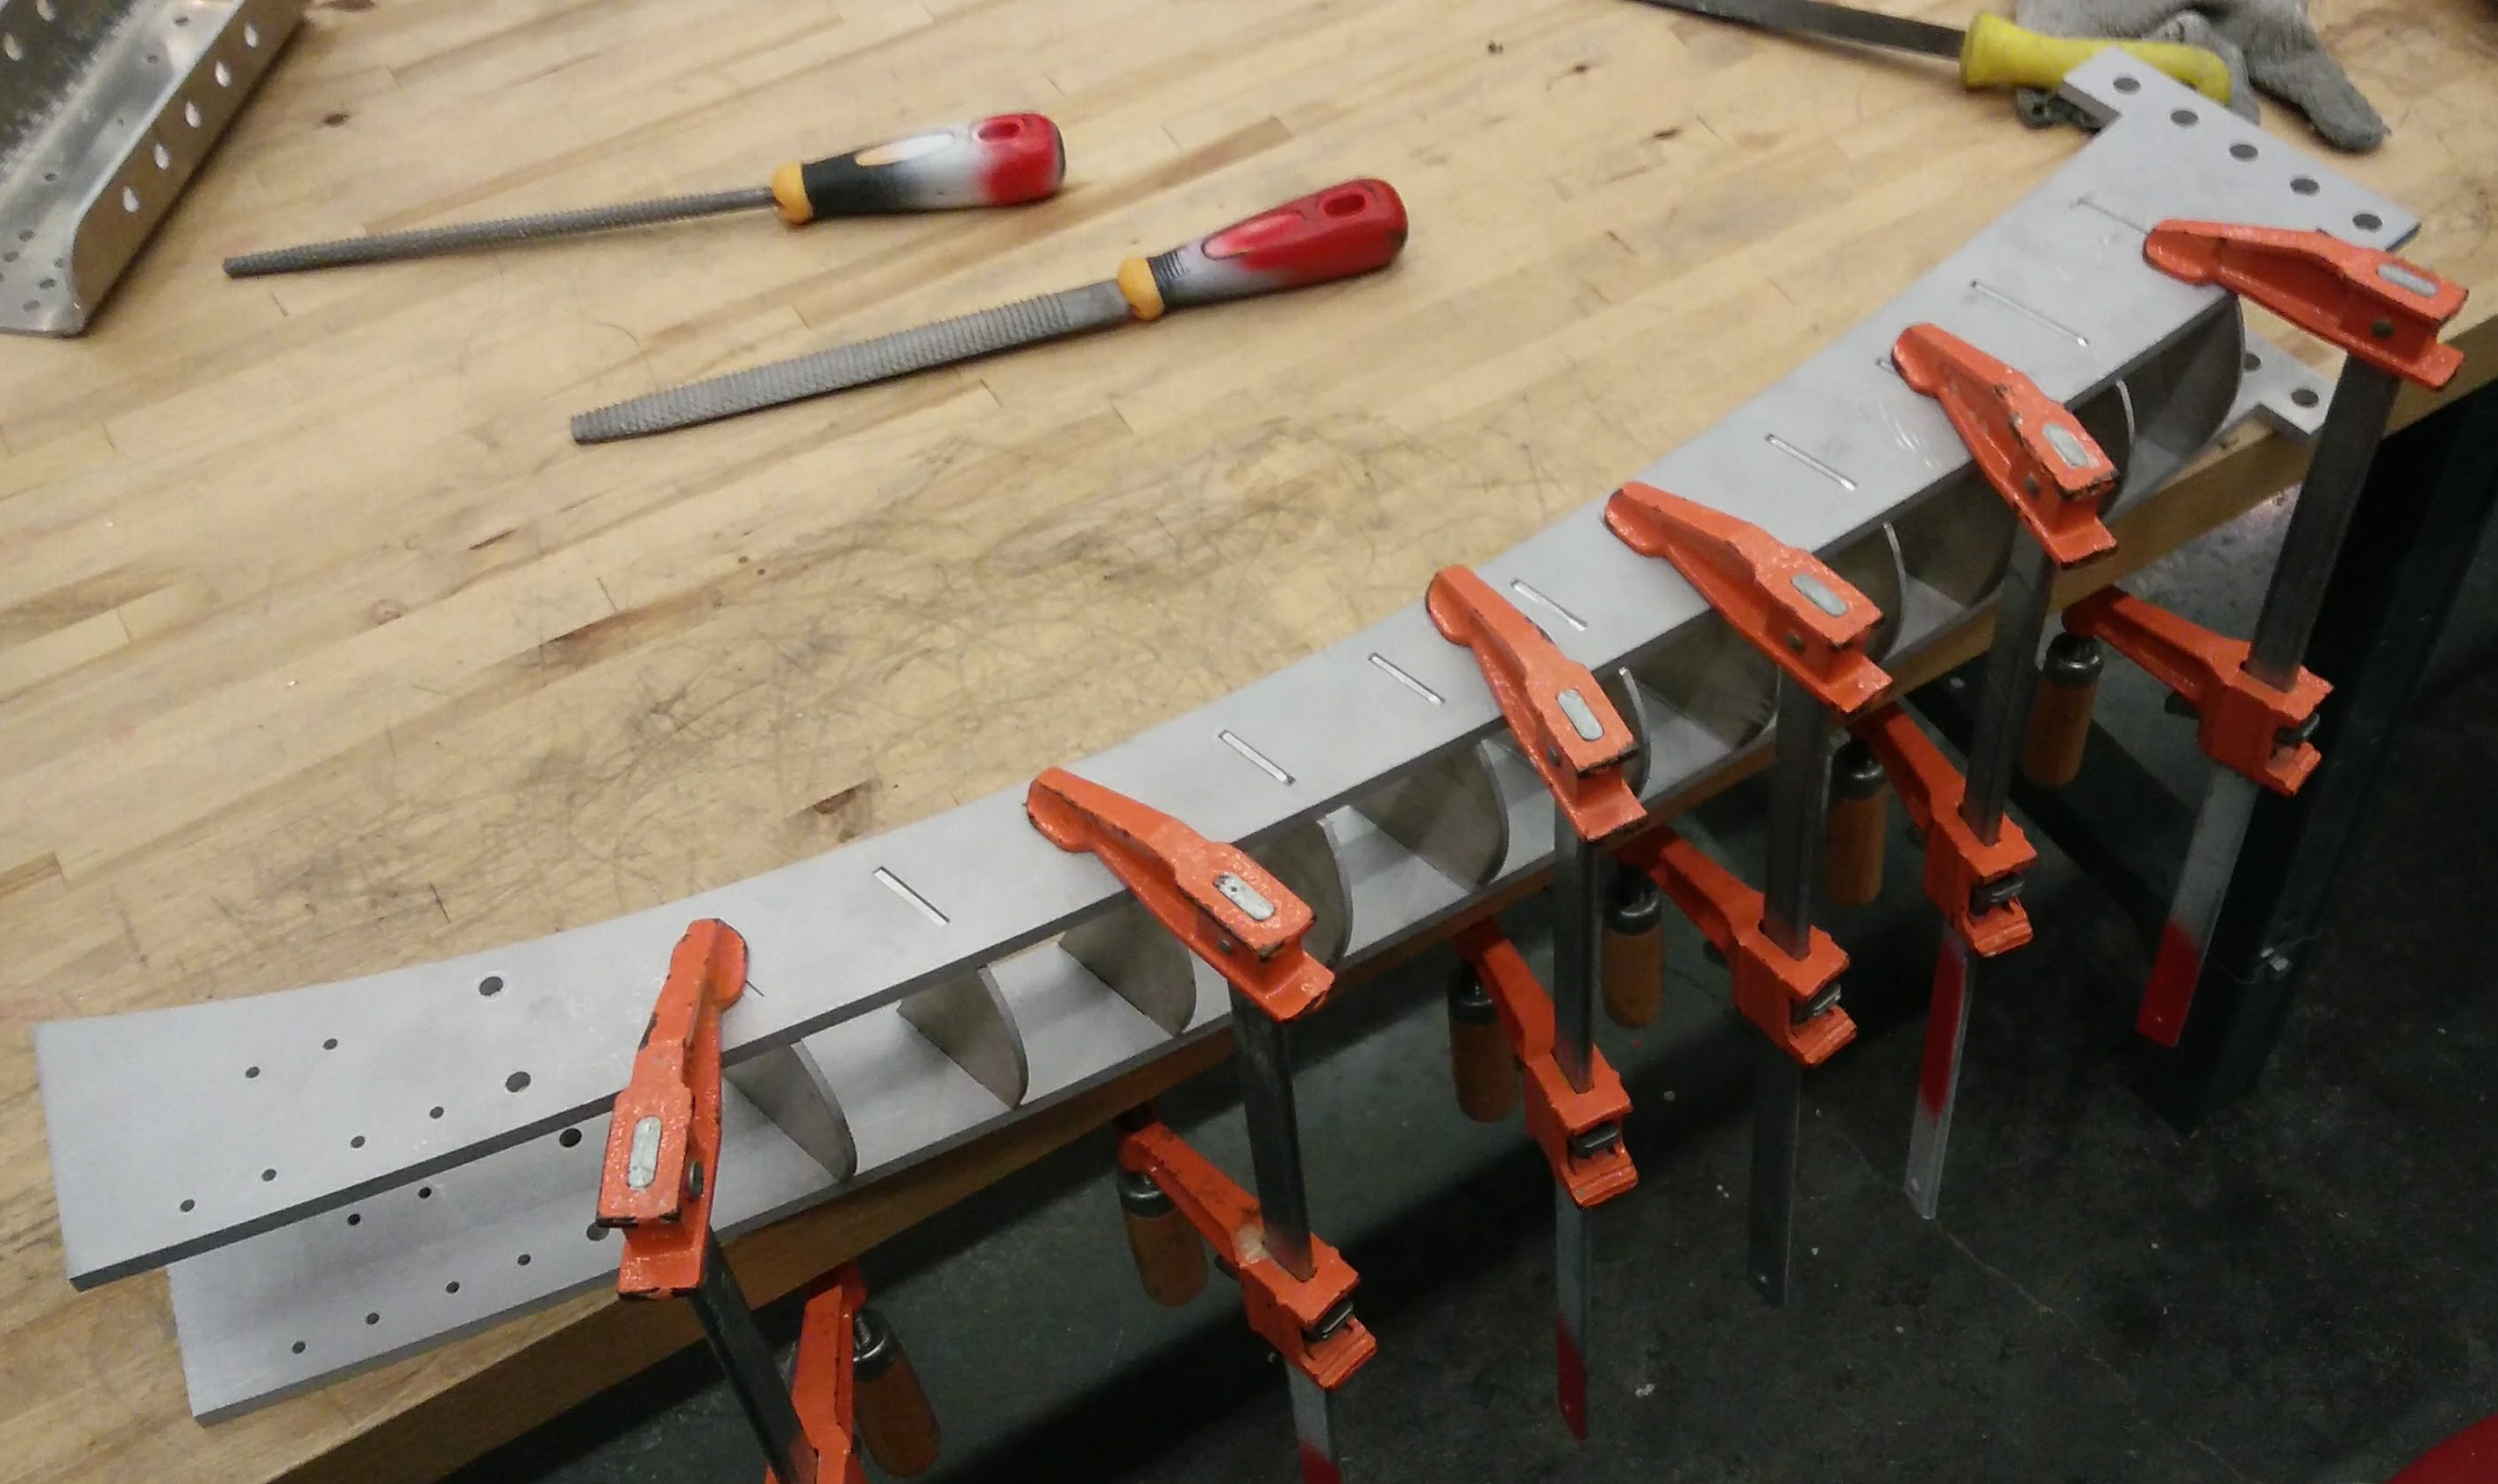
\includegraphics[width=1\linewidth]{figs/05/IMG_20170207_154911}
	\caption{Assembly of the handle bar column}
	\label{IMG_20170207_154911}
\end{marginfigure}

At the bottom of this column there was enough room for allocating the wiring and the Arduino boards. The attachment to the frame was done with a bended aluminum part. It is important to point out that it was decided to fabricate the PEV without using the milling machine. Apart from the time that the milling process takes by itself, a training and a preparation of the necessary files for its production were necessary.

\begin{marginfigure}[0cm]
	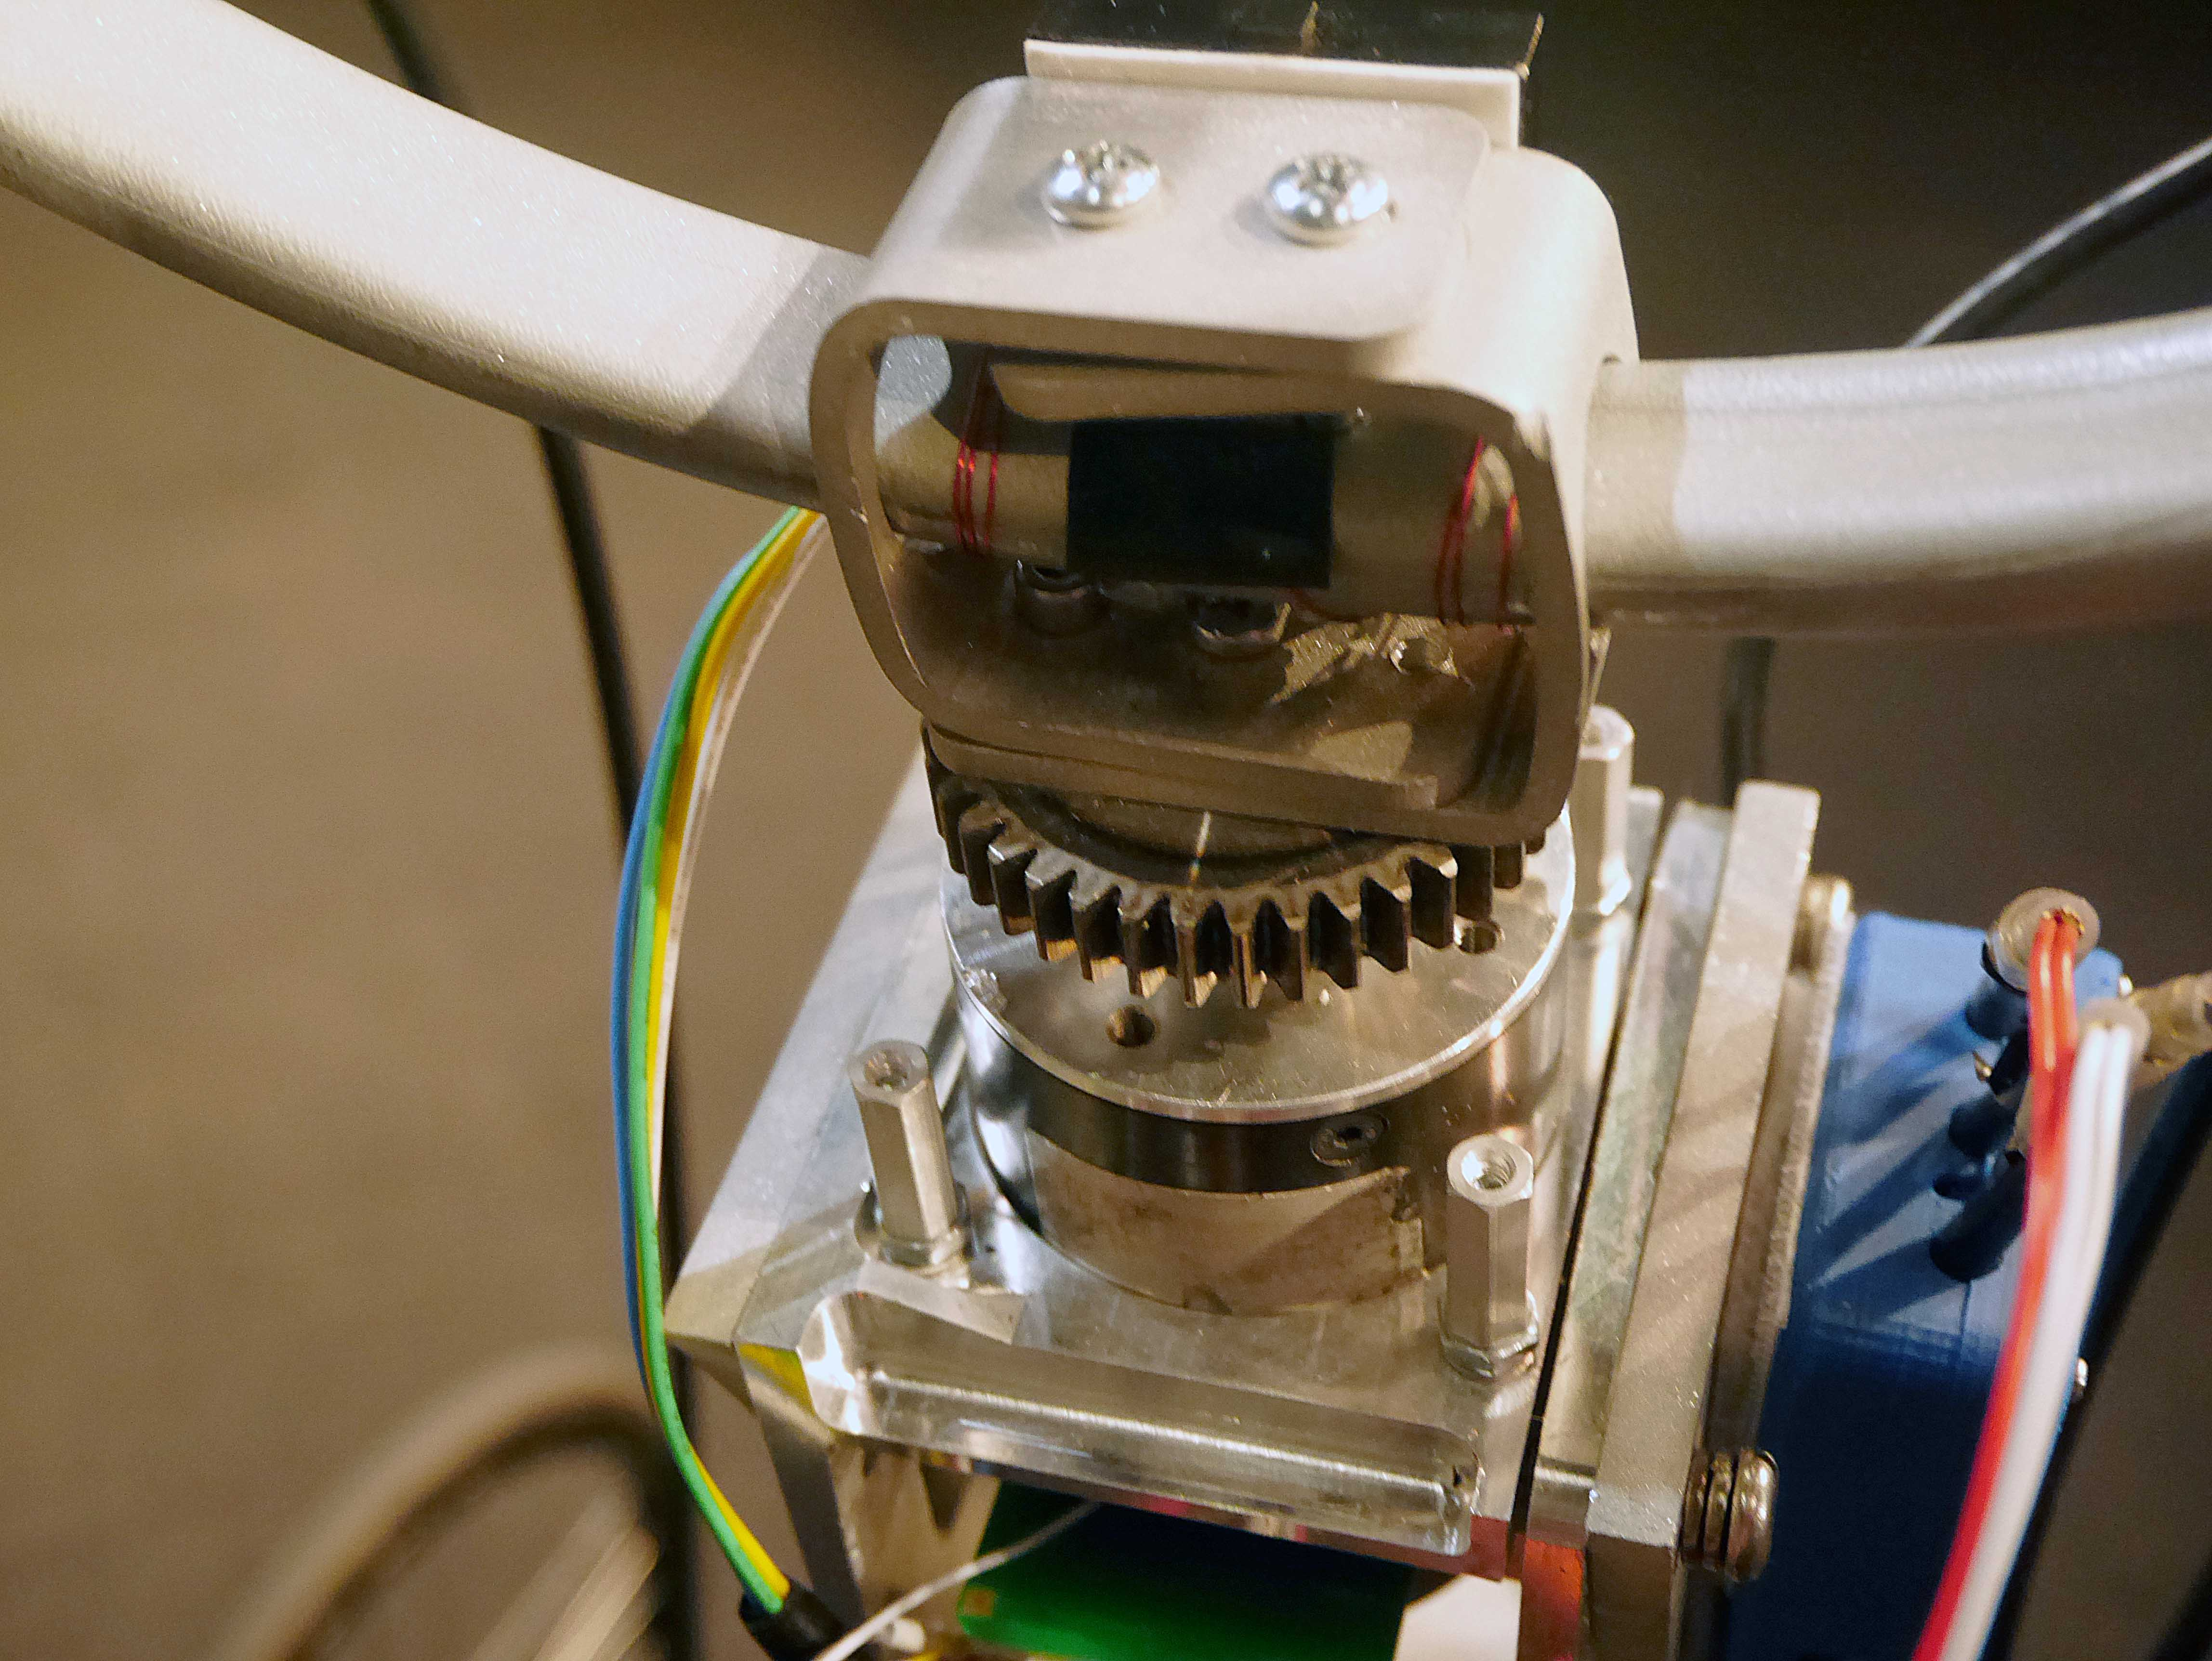
\includegraphics[width=1\linewidth]{figs/05/P1050738}
	\caption{Handle bar: motor joining}
	\label{P1050738}
\end{marginfigure}

On top of the column another NIDEC motor was assembled; its shaft had the handle bar connected (Figure \ref{P1050738}). The reasons to introduce another motor in the handle bar are summarized as follows:
\begin{itemize}
\begin{itemize}
	\item \textbf{Haptic Feedback}: a fundamental part of the steer-by-wire system is to give feedback to the driver about the forces that the steering motor is withstanding. In this way, the driver will have a subconscious input about the forces required to move the wheels, and the user experience will be enhanced. 
	\newpage
	This is also important in term of safety. Moving the handle bar without any friction can be dangerous, since the driver can make sudden turns, leading to a crash or fall.
	
	The implemented feedback was not a realistic input from the forces happening in the steering motor. Instead, the force to move the handle bar linearly increased with the steering angle and the vehicle velocity. There was also a limit in the maximum input angle, generating enough force to block any motion. To do so, the motor variables read from the VESC controller were used, mainly the battery current, the motor current and the tachometer.
	
\begin{figure}[h!]
	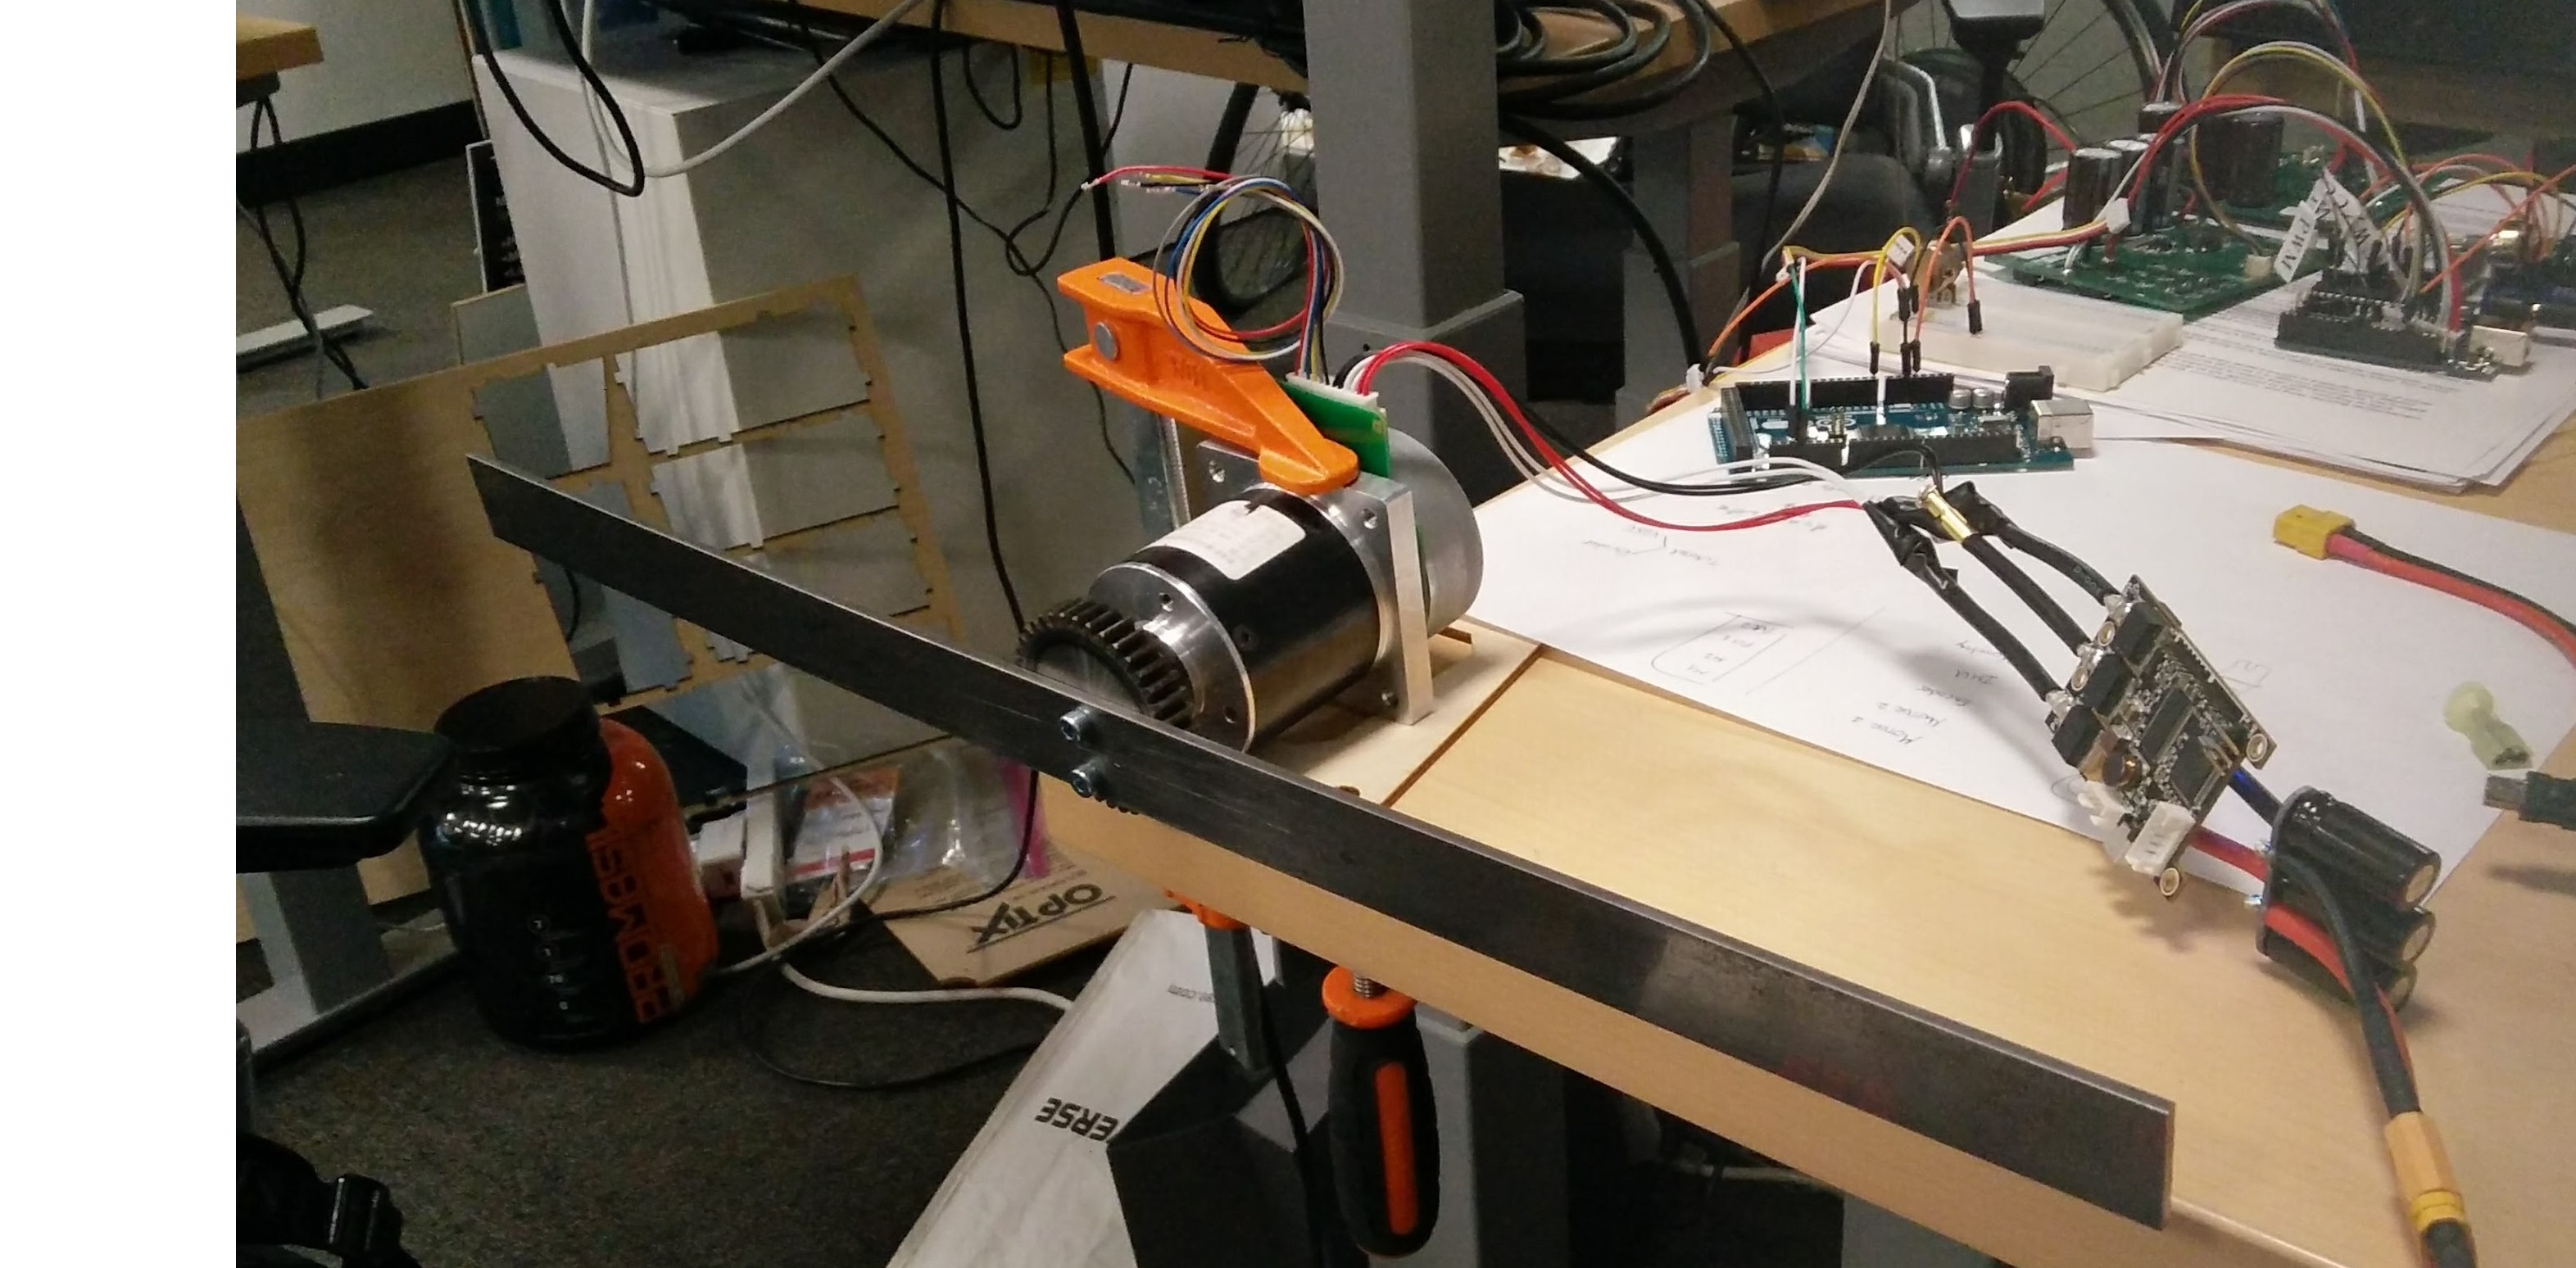
\includegraphics[width=1\linewidth]{figs/05/IMG_20170123_121416}
	\caption{Test bench for the haptic feedback}
	\\[-1cm]
\end{figure}
	At low speeds, the angle range was quite wide --but limited-- and the forces required to move the handle bar were low. At higher speeds, the handle bar was very limited to a low range of angles and also it required a lot of force to move the handle bar.	This helped to reduce the speed of steering, and protected the user to exceed the steering input at high speeds.
	
	\item \textbf{Alert/notify user}: Apart from controlling the steering input from the driver, a motorized handle bar can warn the driver about an obstacle in the road or any other issues with the vehicle or the road conditions. Vibrating the handle bar can the fastest way to notify the user about any problem, reducing the time of reaction and thus protecting the user.
	
	\item \textbf{Compass}: A possible scenario when riding the PEV can be the indication to go right or left when an address has been indicated to the system. Sometimes when riding a bike in a new city or in a unknown neighborhood it is necessary to stop an check the map to orient ourselves and find the next spot.
\end{itemize}
\end{itemize}
\newpage

The handle bar contains a grip and a brake on each side and a potentiometer on the right side (Figure \ref{handle_bar}). The left and right brakes activate the brakes on the left and right front wheels respectively, and the potentiometer activates the power assist on the rear motor. A higher value of the potentiometer means a higher duty cycle in the rear motor, thus increasing the velocity of the vehicle.
\begin{marginfigure}
	\caption{Handle bar}
	\label{handle_bar}
\end{marginfigure}
\begin{figure}[h]
		\minipage{0.5\textwidth}
		  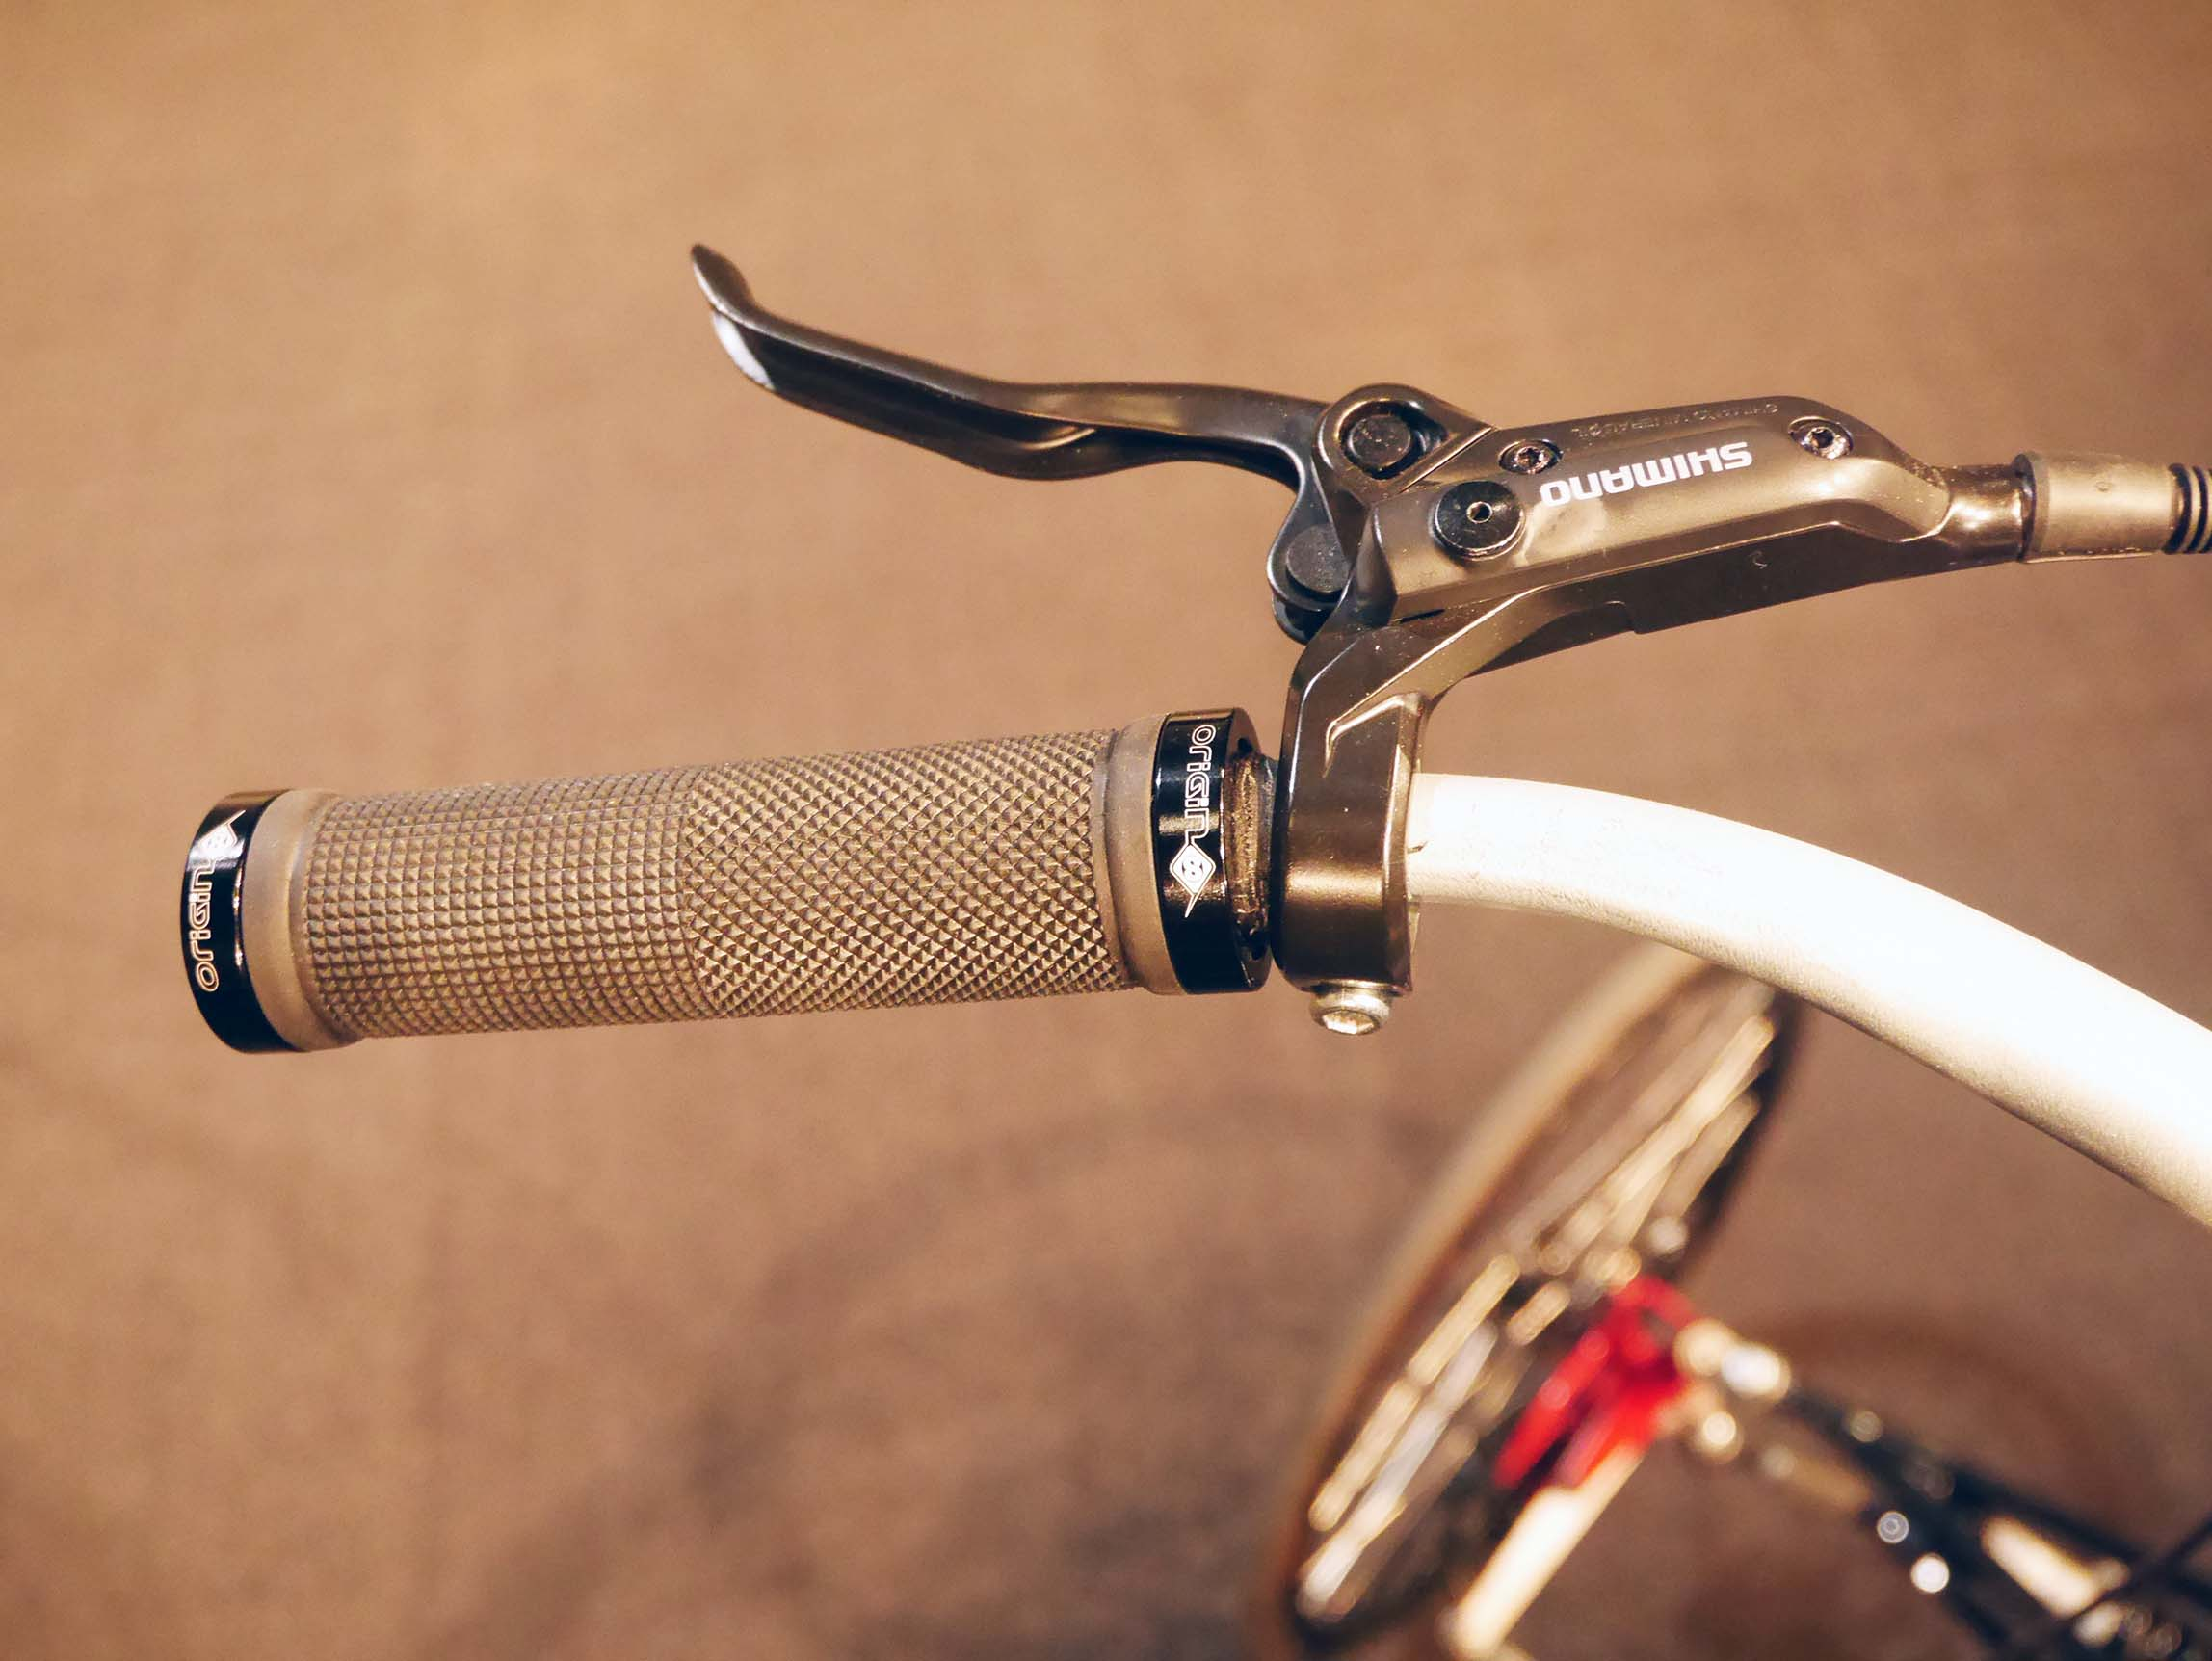
\includegraphics[width=1.0\linewidth]{figs/05/P10507342}
		  \captionof{a)}{ Left grip and brake}
		\endminipage\hfill
		\hspace{1pt}
		\minipage{0.5\textwidth}
		  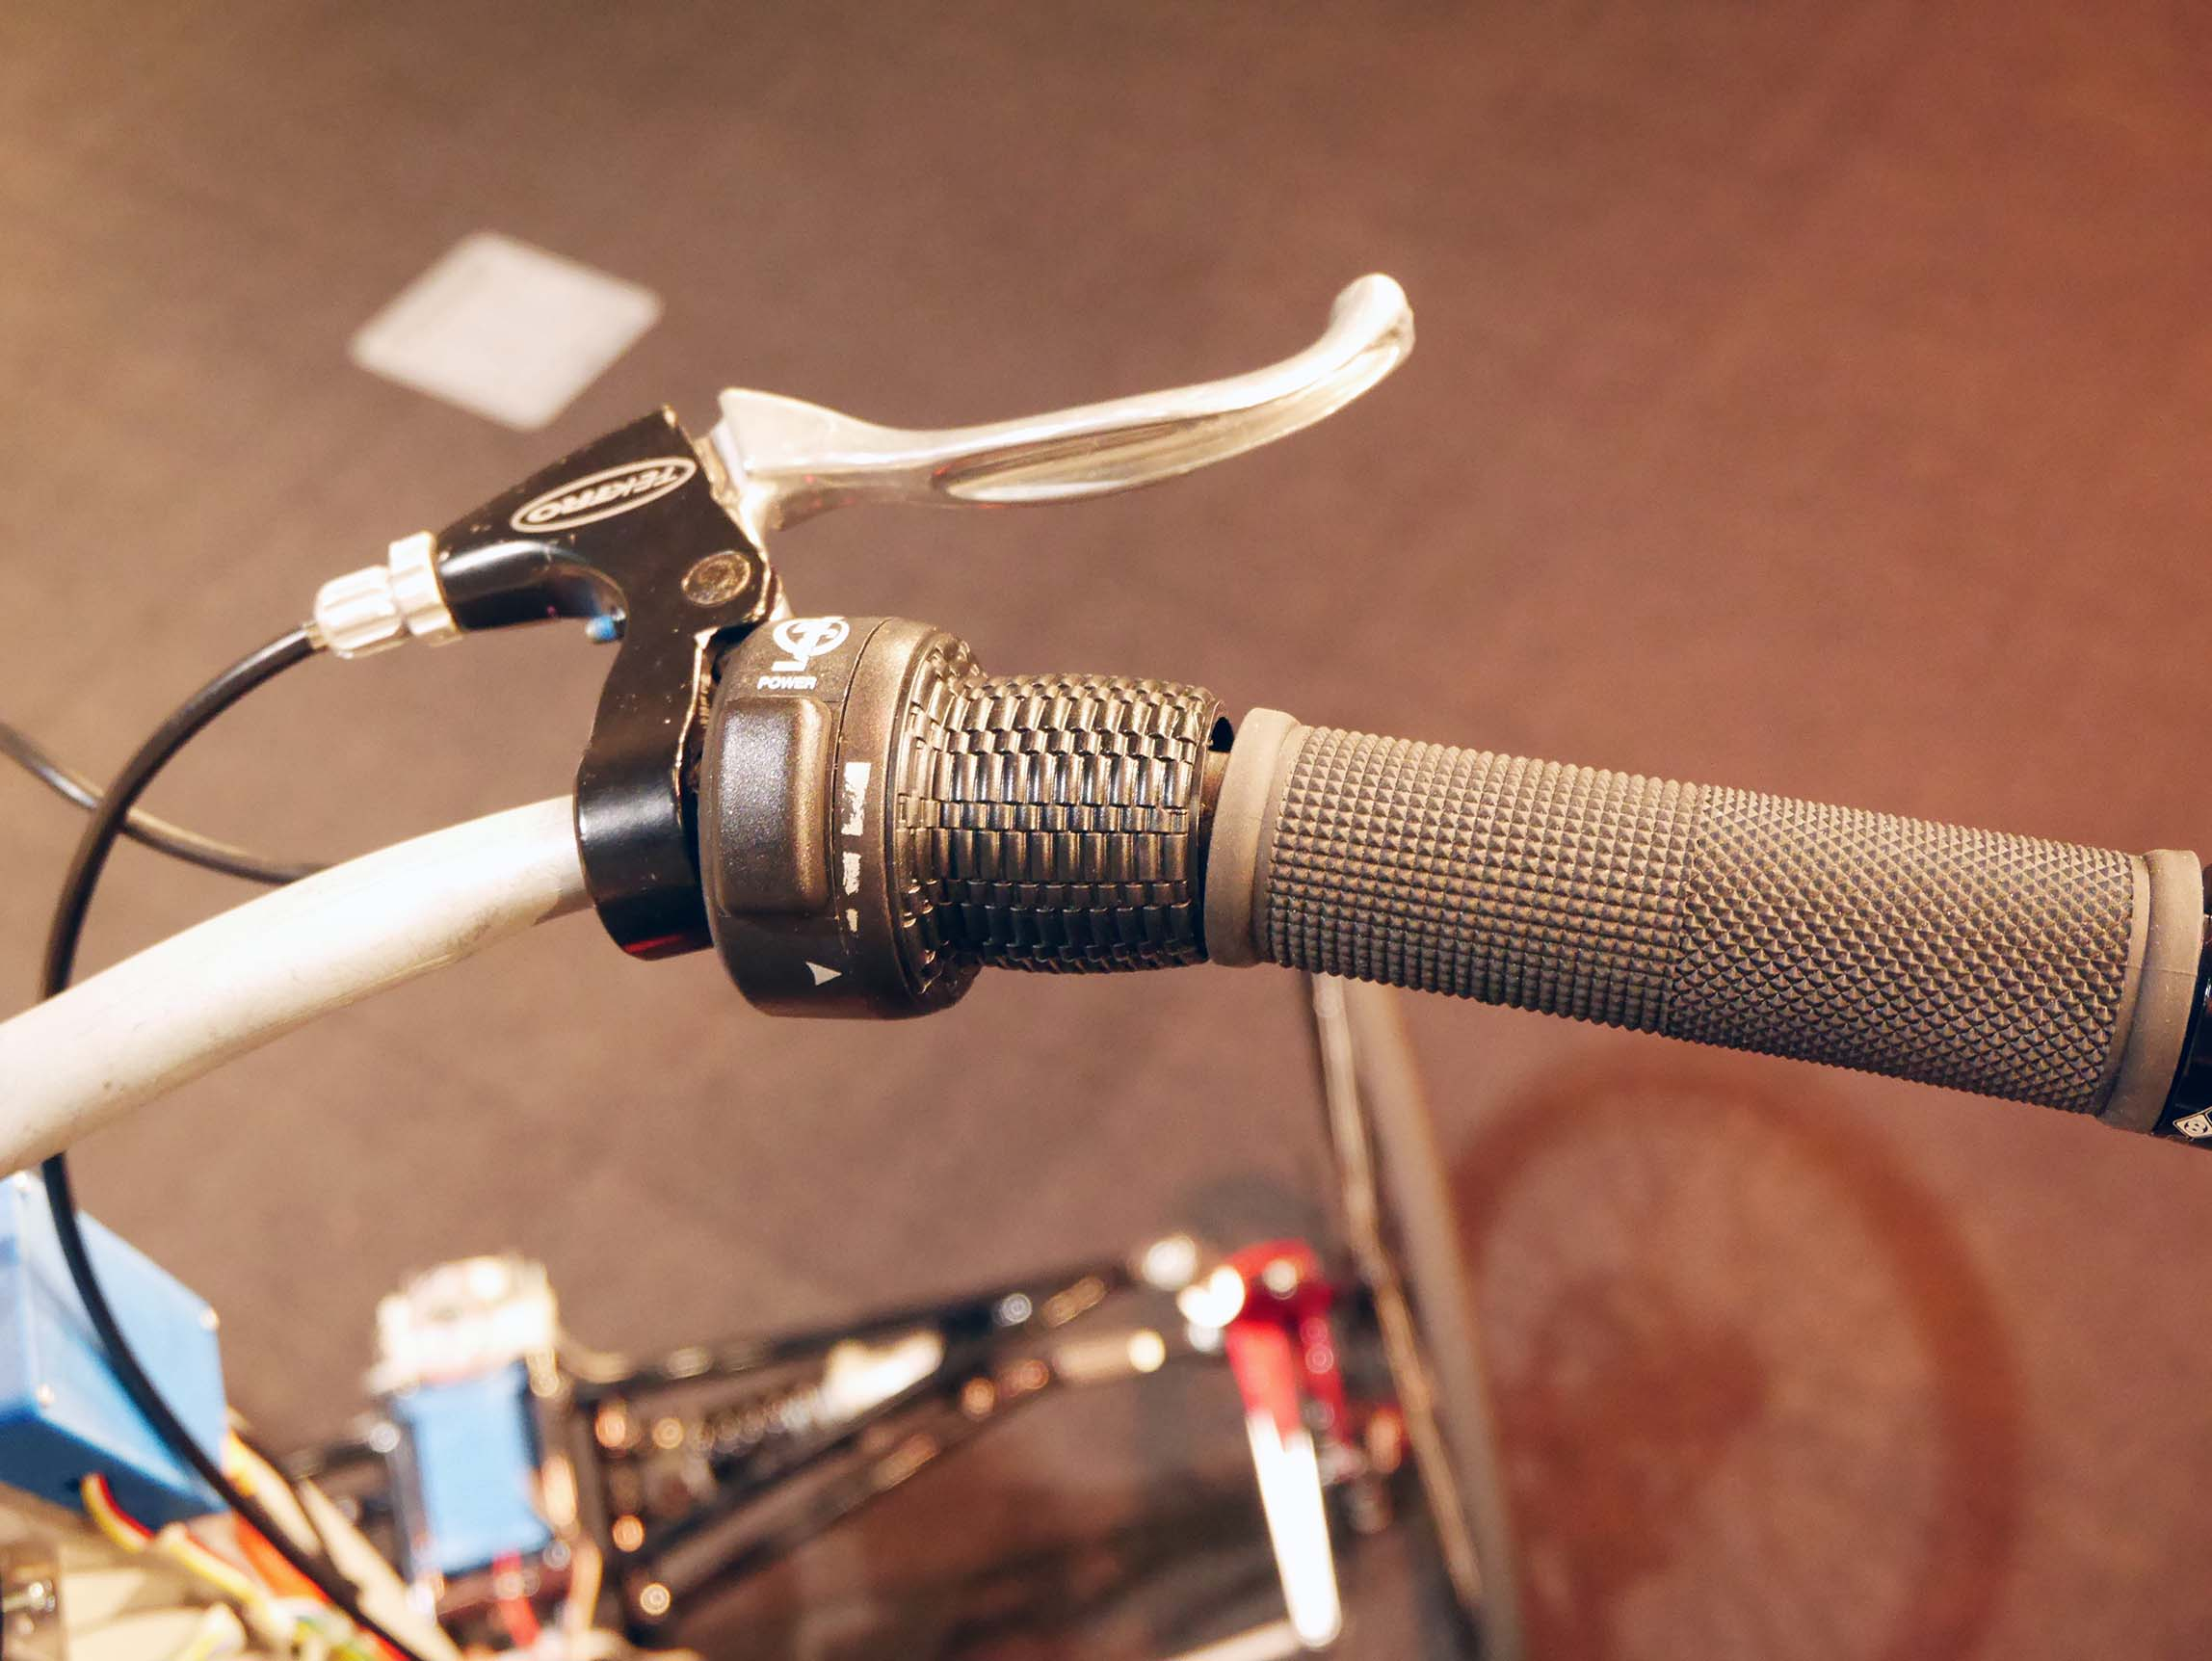
\includegraphics[width=1.0\linewidth]{figs/05/P10507332}
		  \captionof{b)}{ Right grip, brake and throttle}
		\endminipage
		\\[0pt]
\end{figure}

\textbf{Driver ergonomics}

The height and the position of the handle bar was designed to follow the indications in the book "The Guide to Cycling Ergonomics" by Ergotec\cite{ergonomics}. The angles of the driver's articulations have been included in the drawings appendix.

\begin{figure}[h!]
	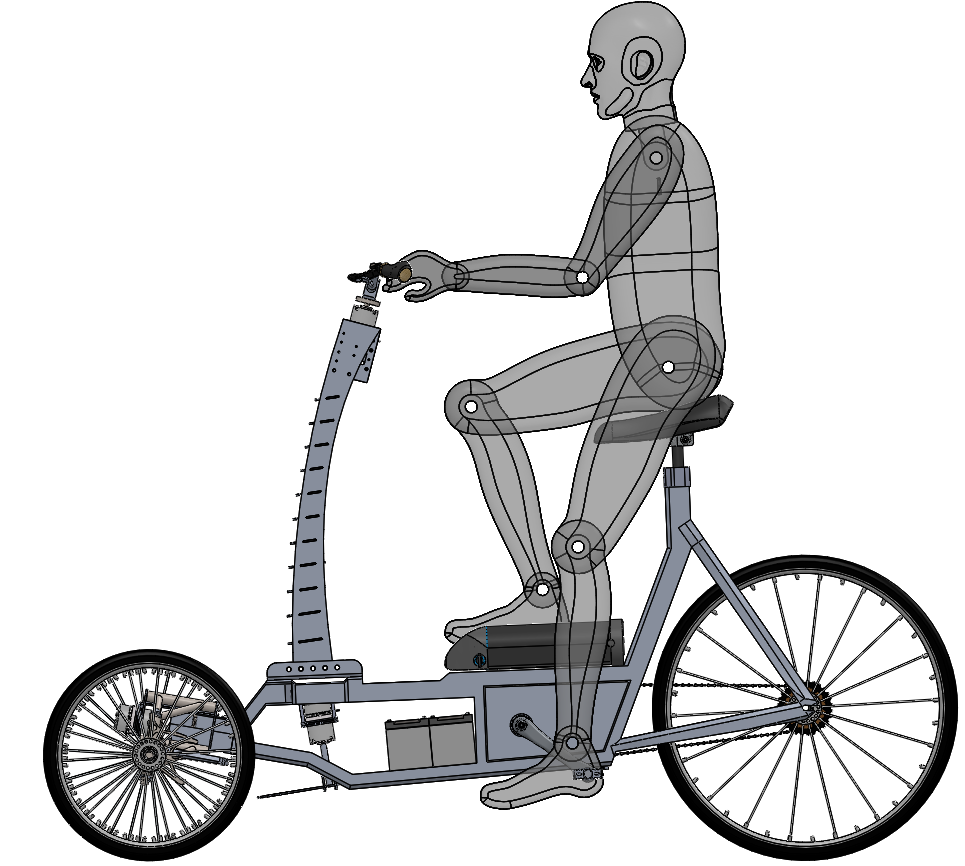
\includegraphics[width=1\linewidth]{figs/05/driver2}
	\caption{Driver position on the CAD model}
	\\[0cm]
\end{figure}

\newpage
\subsection{Power Assist}

The PEV is power assisted by a brushless motor located in the rear wheel's hub. This motor is a 36V E-Bikeling 500W geared motor\cite{ebikeling}. It provides enough power to assist the propulsion of the PEV. The system comes prepared to attach a sprocket to the hub, so that the rear wheel can be moved with the pedals. All the drivetrain parts were mounted in the frame.

The rear brushless motor, as every NIDEC motor (tilting, steering, handle bar), are controlled by VESC. In the next section --electronics-- more detailed information is included. The PEV is intended to be a lightweight vehicle fully prepared to incorporate a modular autonomous package. This kit will transform a normal three wheeler vehicle into an autonomous urban vehicle. That is why a motor to propulse the vehicle is necessary, as well as another motor to steer the front wheels.

\begin{marginfigure}[0cm]
	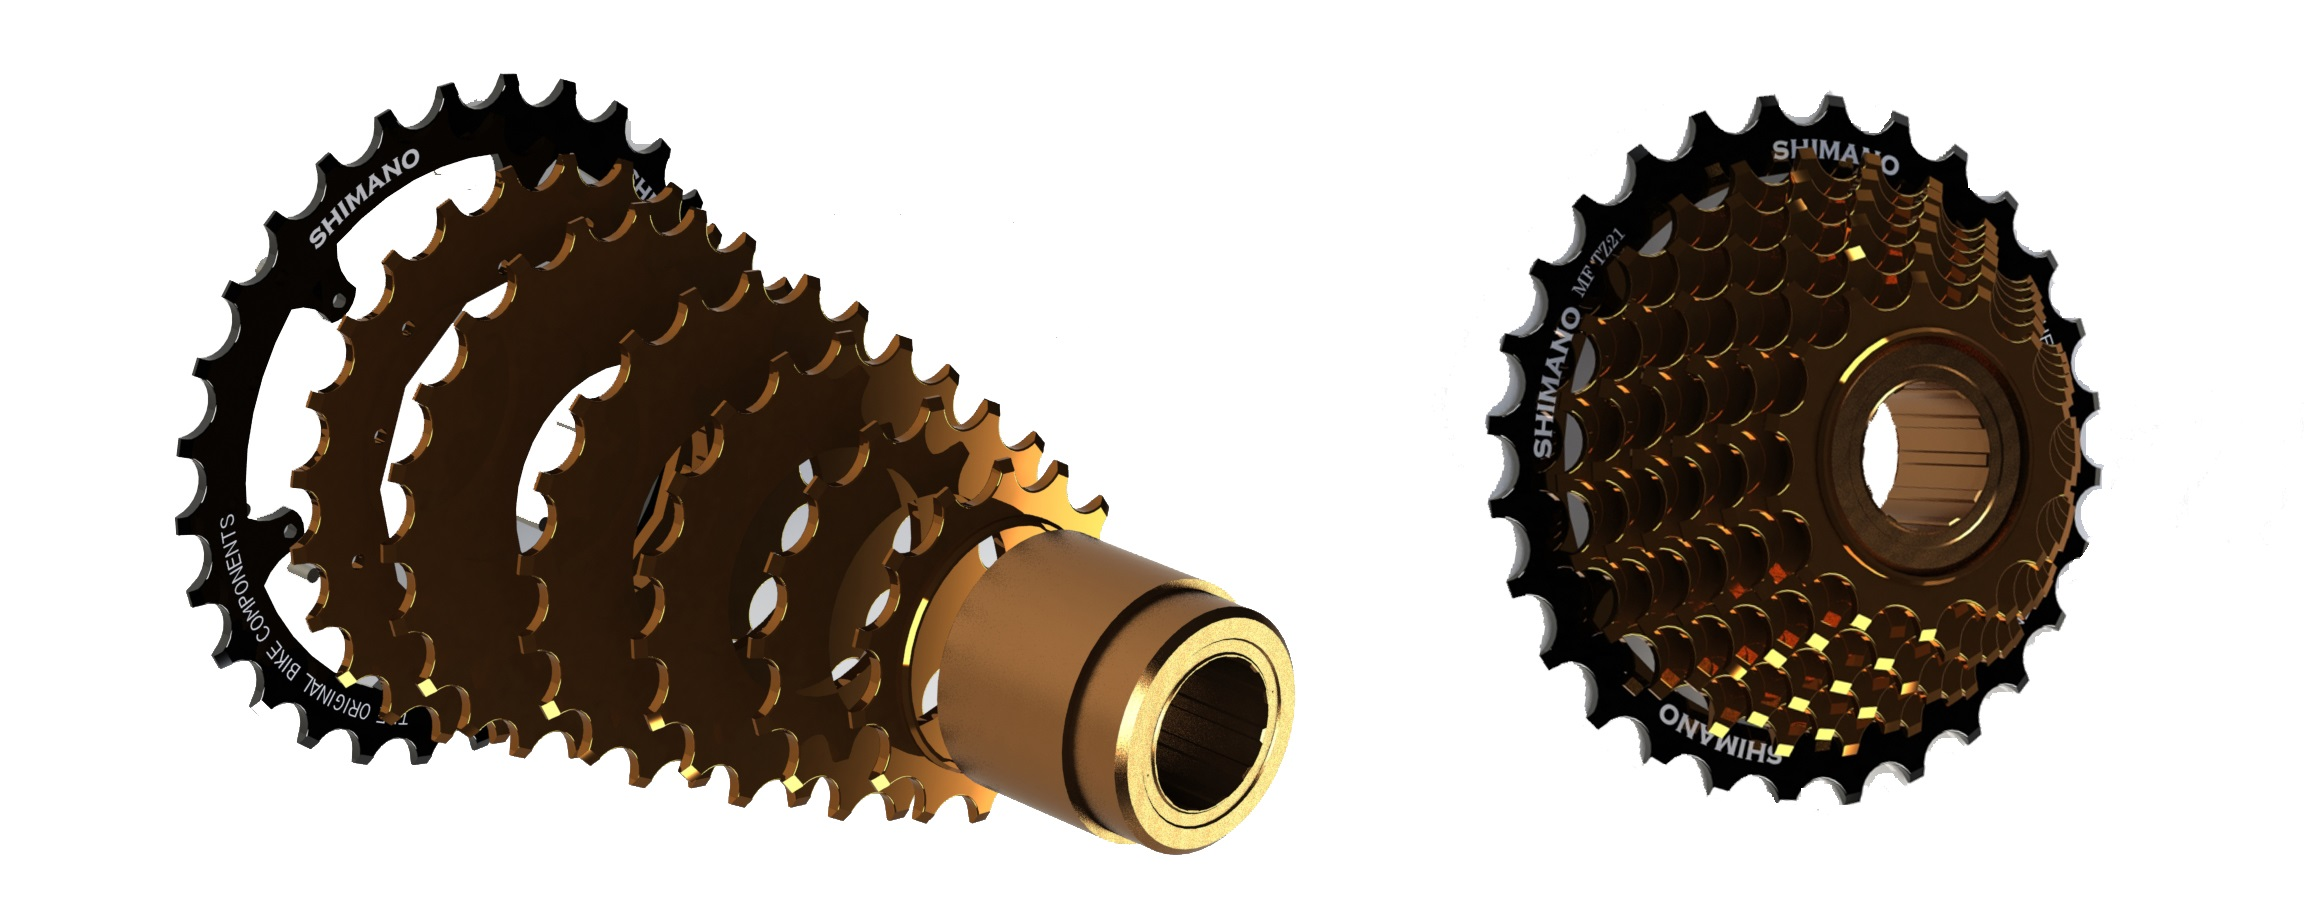
\includegraphics[width=1\linewidth]{figs/05/Sprocket}
	\caption{PEV sprocket}
\end{marginfigure}

The motor will assist under the user demands. In the right side of the handle bar there is a potentiometer that will throttle the vehicle when turned on. Regarding the signal flow, the potentiometer sends the command to the Arduino Mega, which is connected to the VESC controller through serial. The VESC finally controls the motor and moves the rear wheel. 

\begin{figure}[h!]
	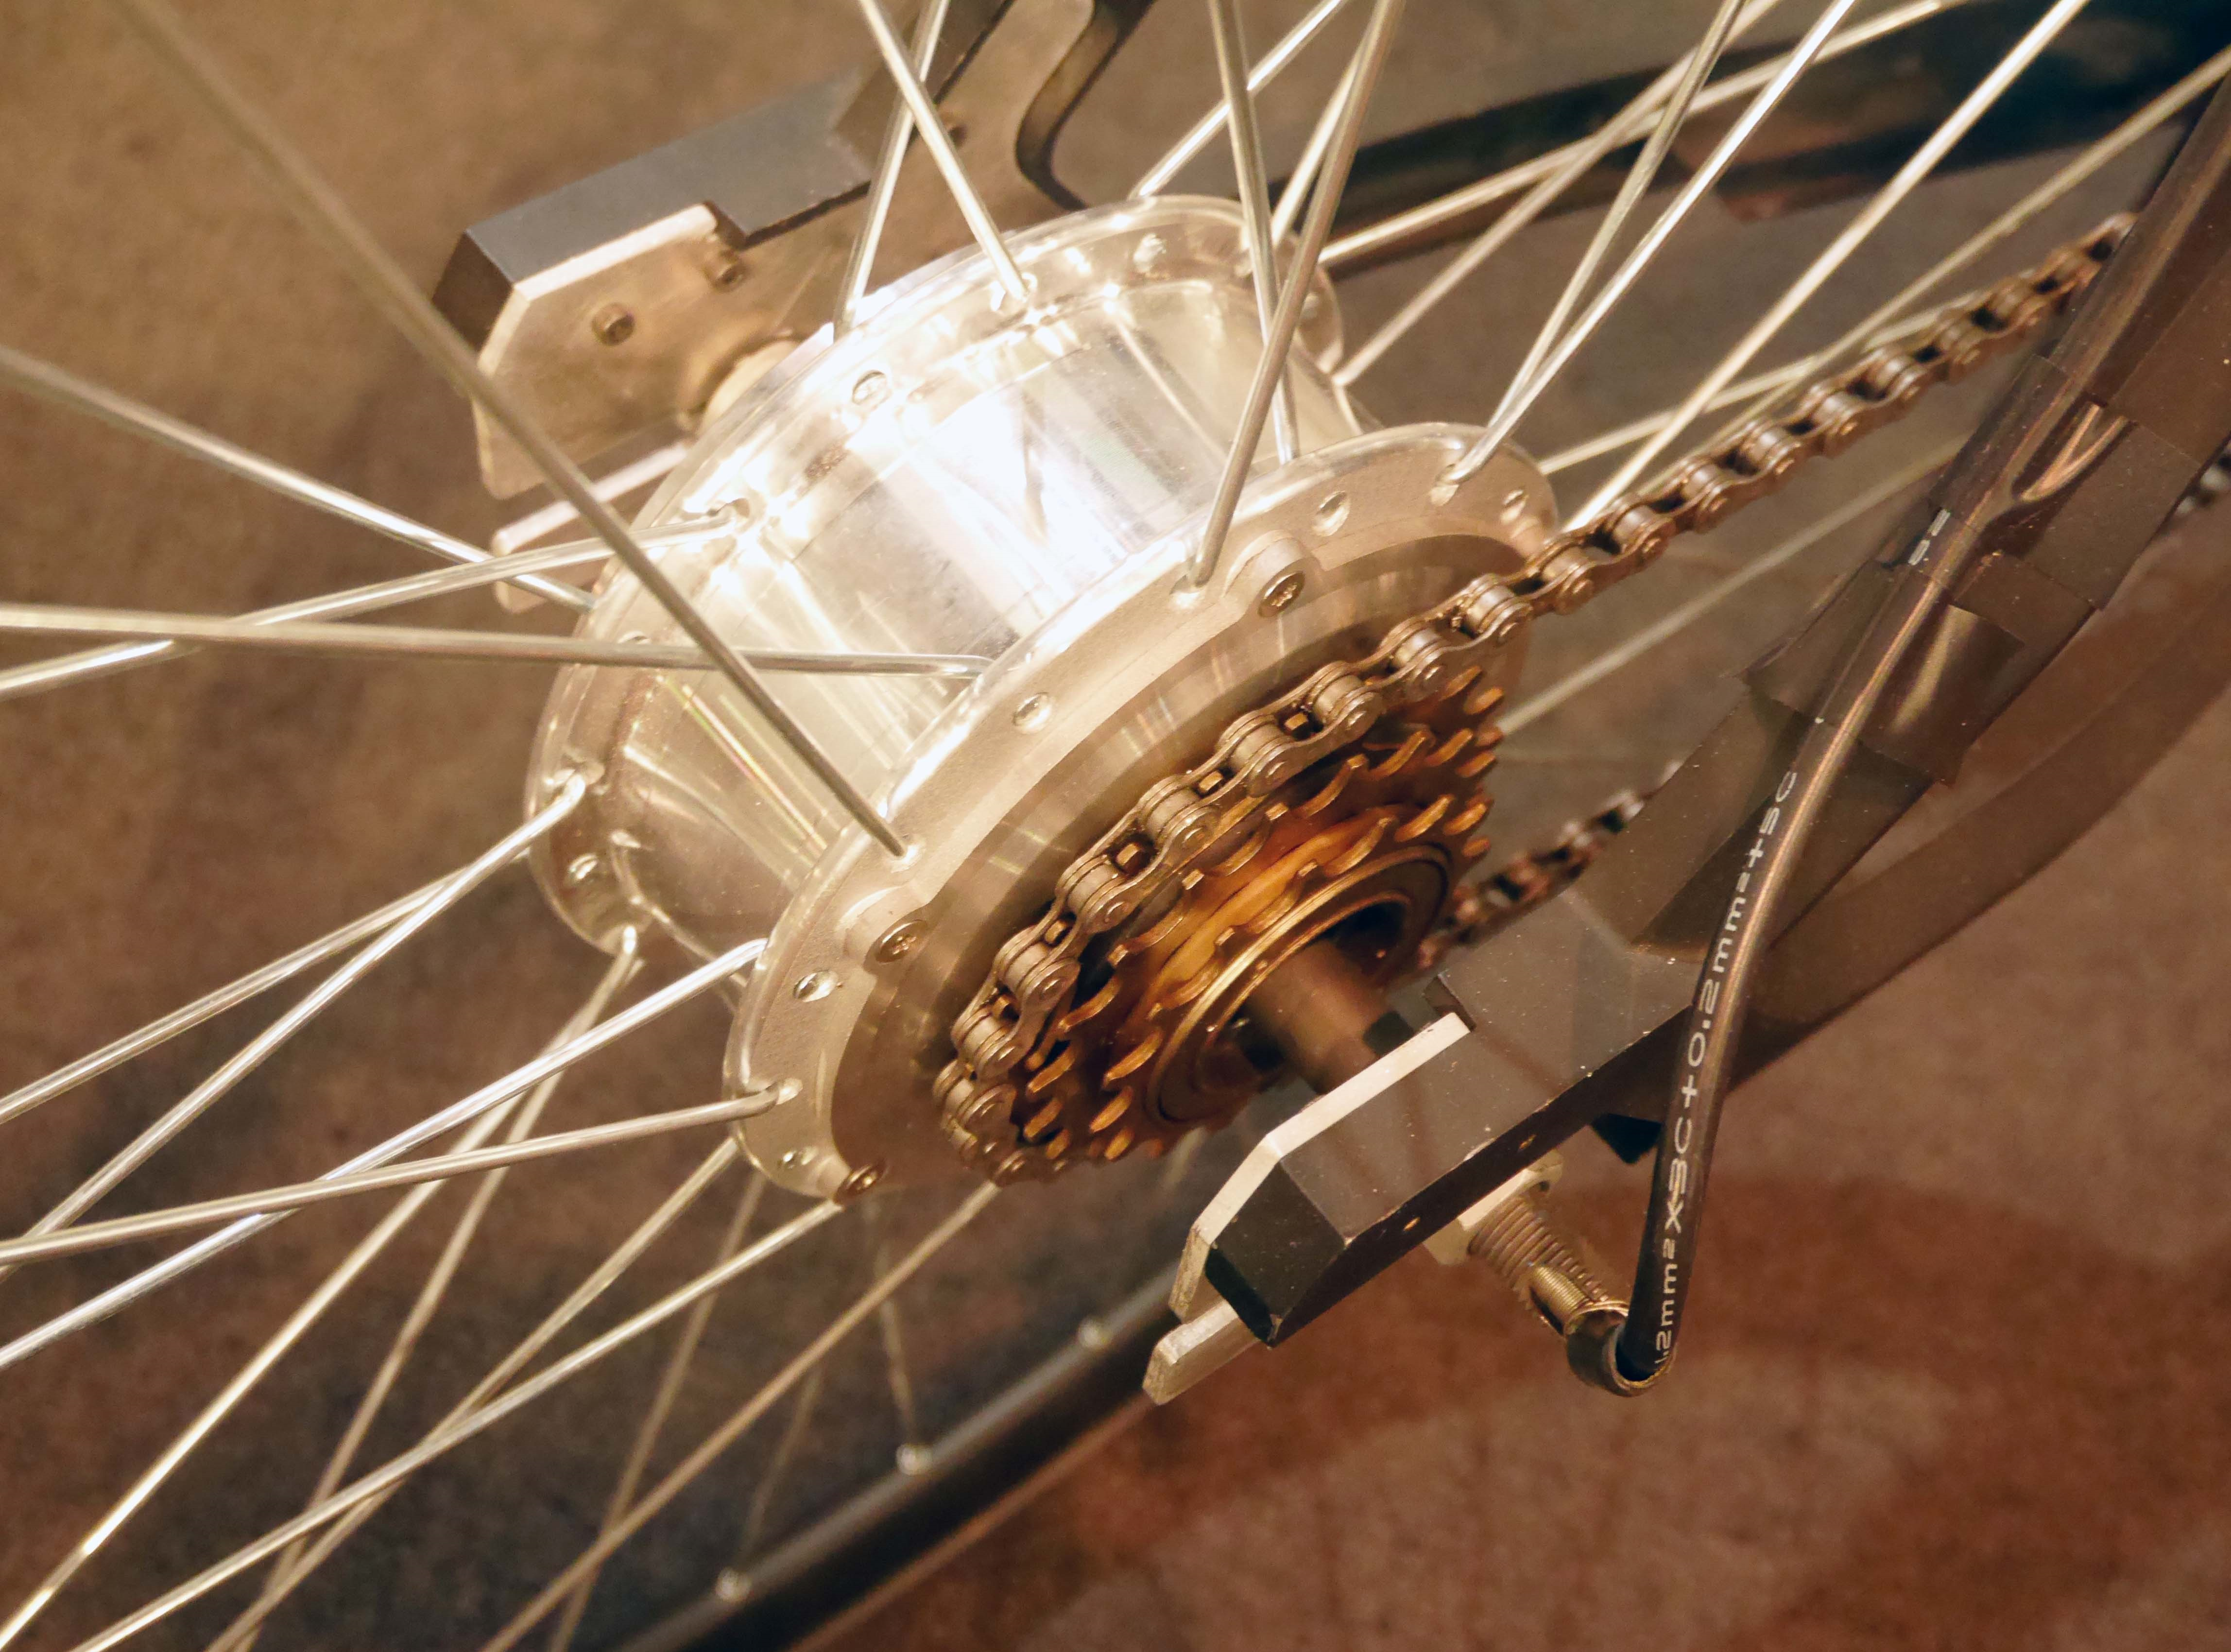
\includegraphics[width=1\linewidth]{figs/05/P1050729}
	\caption{Rear motor in the hub}
\end{figure}

\begin{marginfigure}[-6cm]
	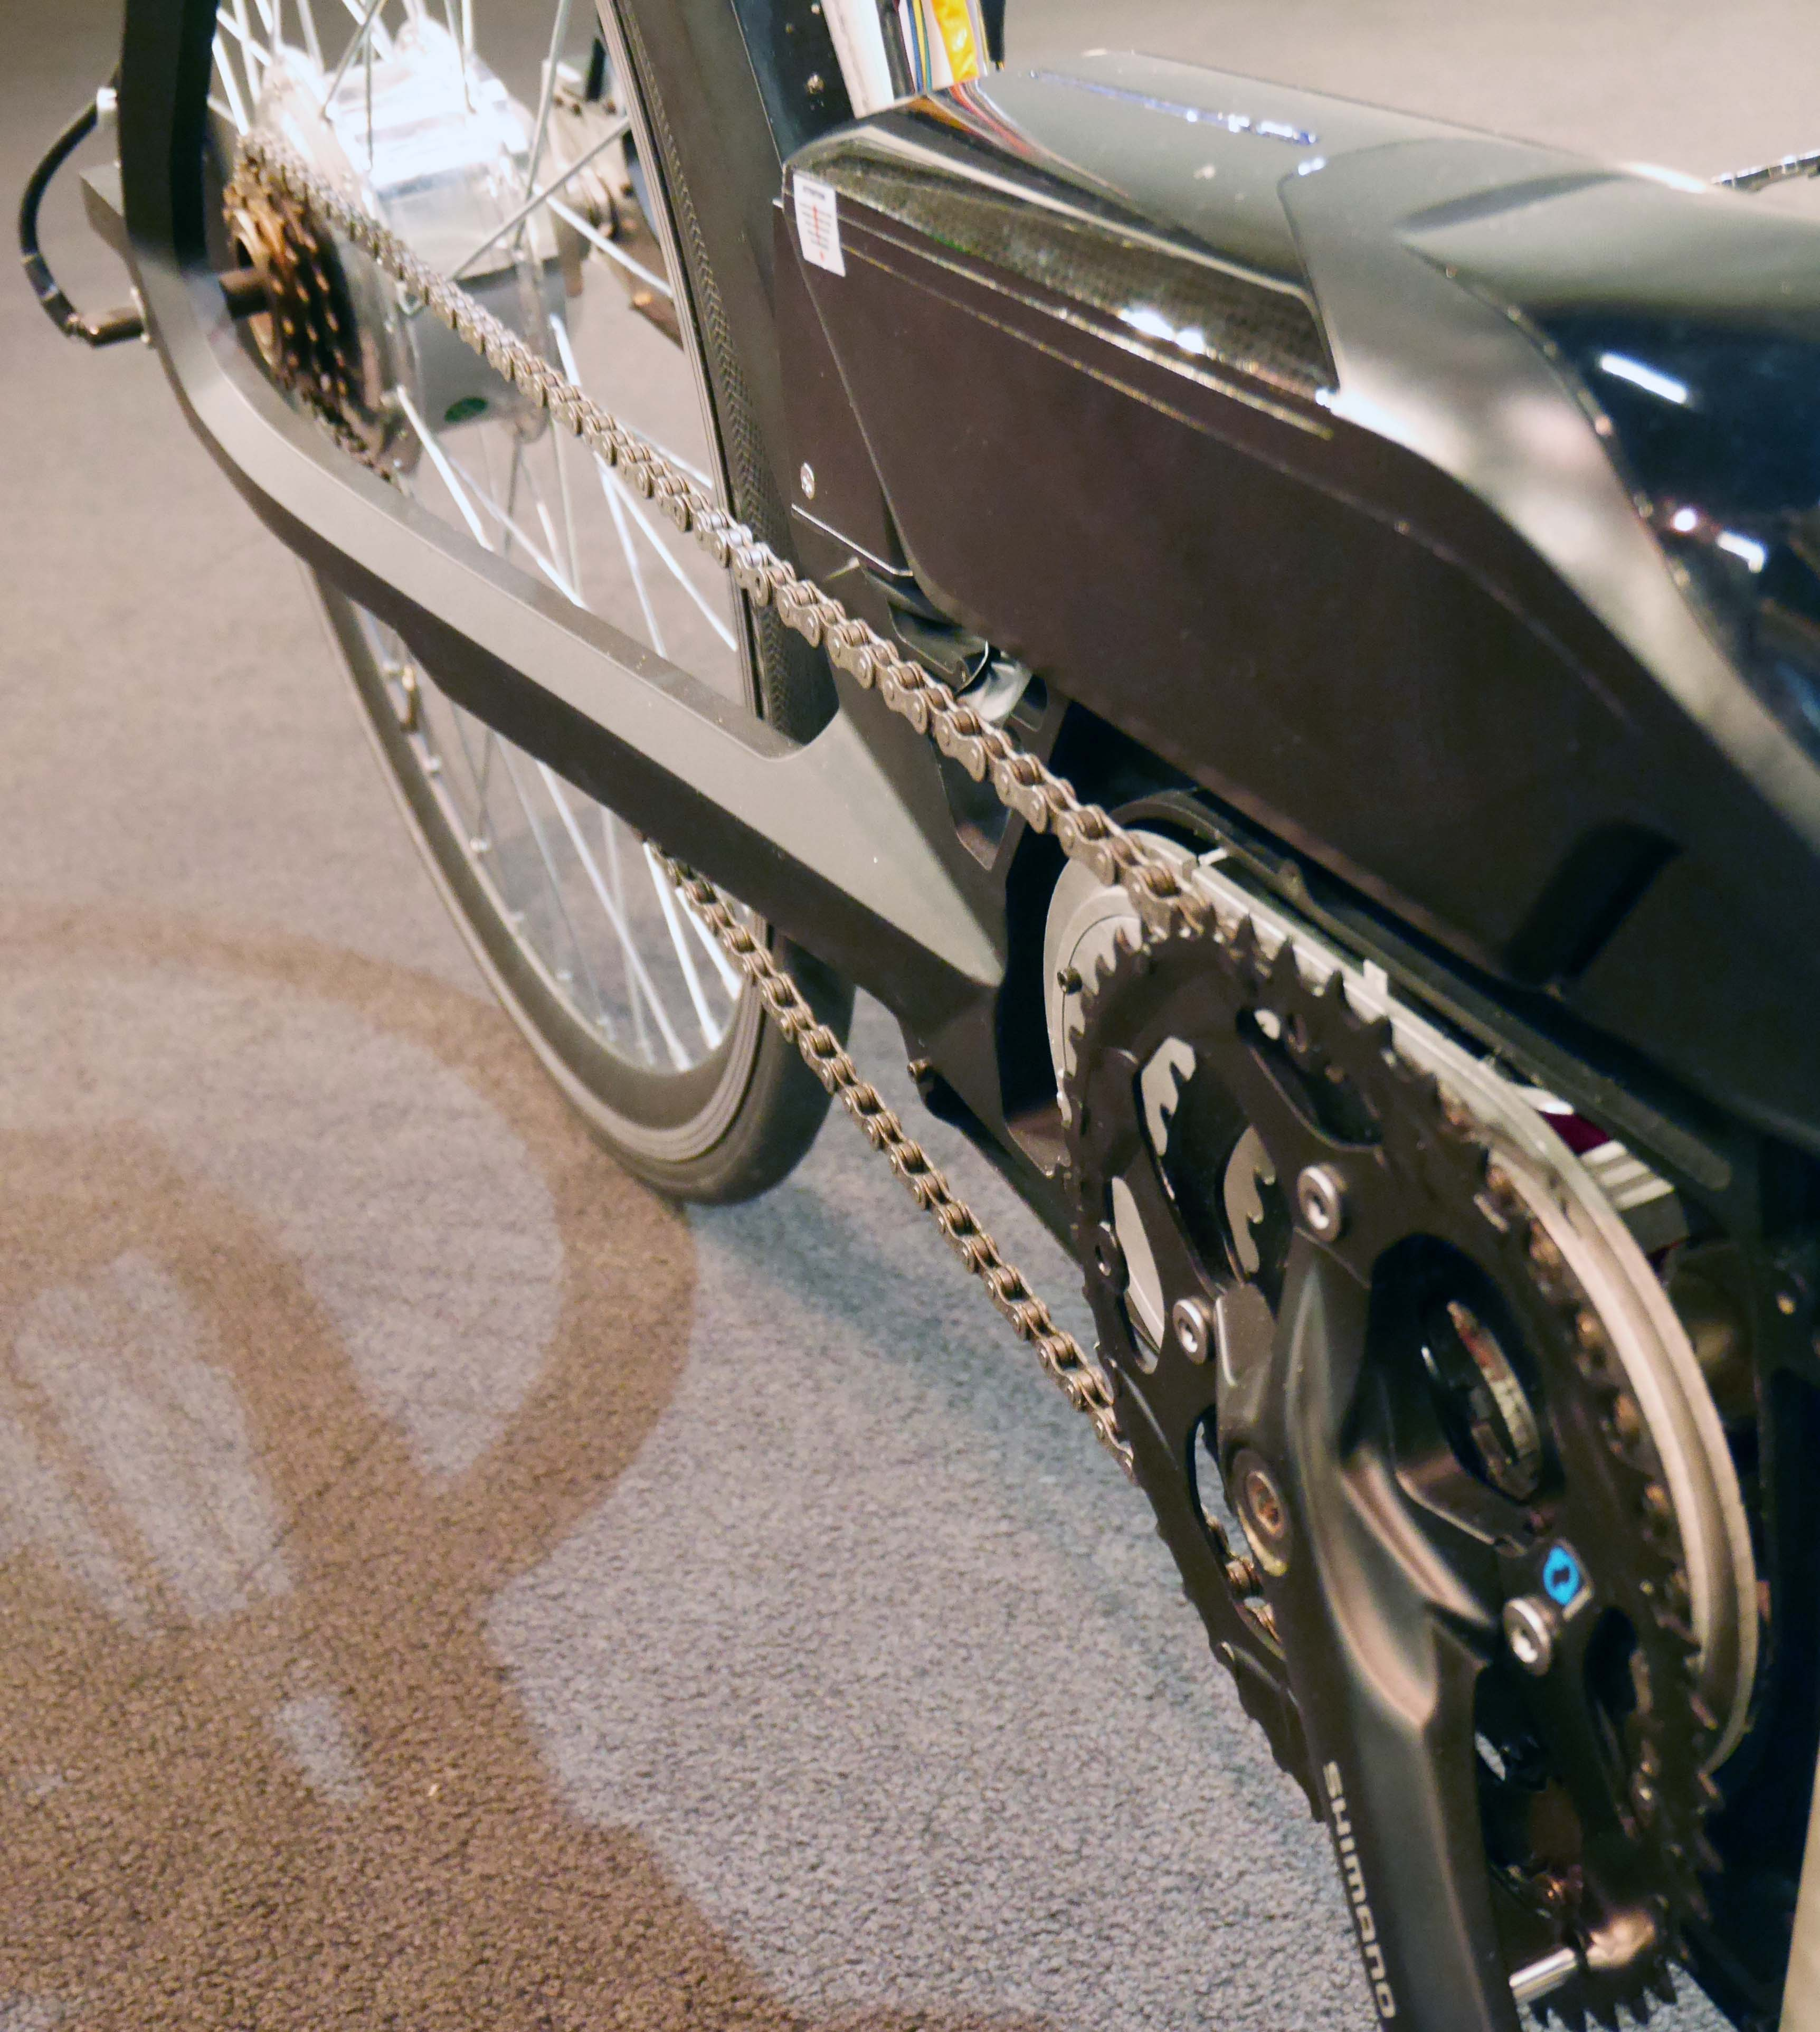
\includegraphics[width=1\linewidth]{figs/05/P1050742}
	\caption{PEV Pedal system: chain, gears and pedals}
\end{marginfigure}

\newpage
\subsection{Renders and Pictures}
\begin{figure}[h!]
	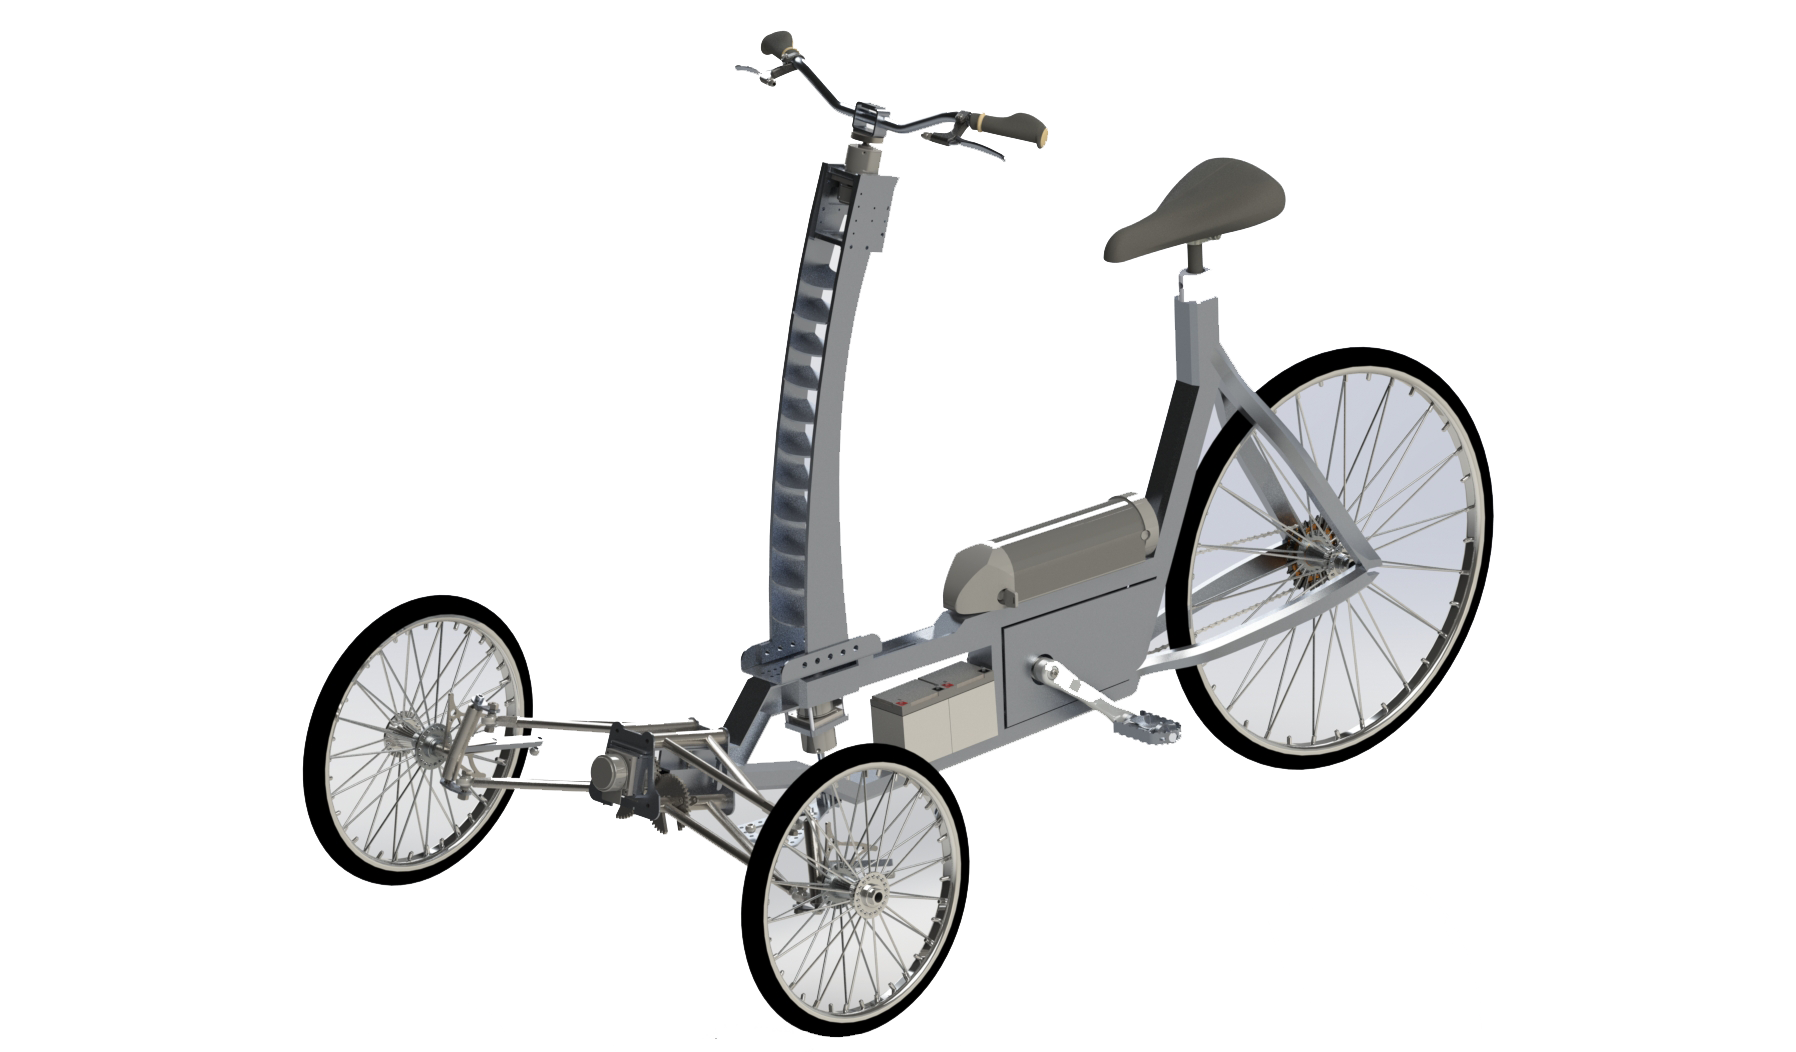
\includegraphics[width=1.15\linewidth]{figs/05/Render_Design_B_3}
	\caption{Isometric render}
	\\[-1cm]
\end{figure}
\begin{figure}[h!]
	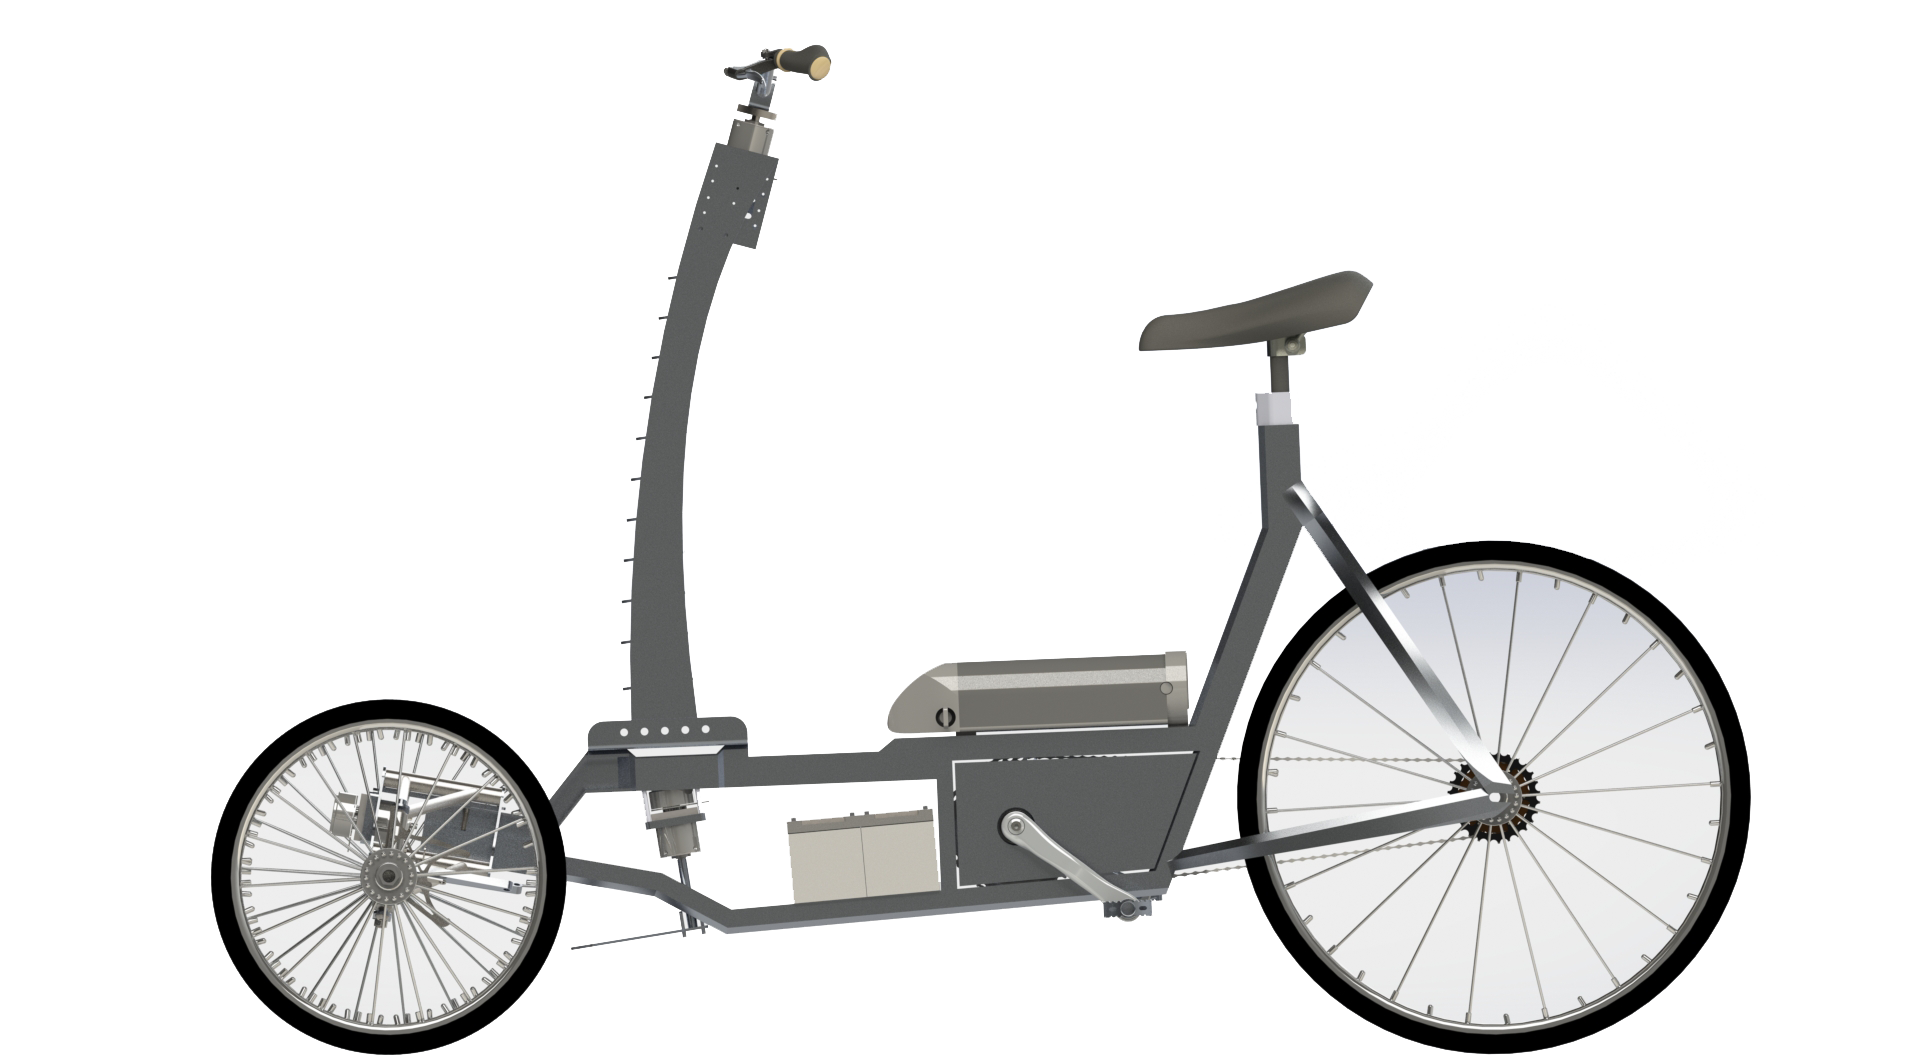
\includegraphics[width=1.1\linewidth]{figs/05/Render_Design_B_4}
	\caption{Lateral render}
	\\[-1cm]
\end{figure}
\begin{figure}[h!]
	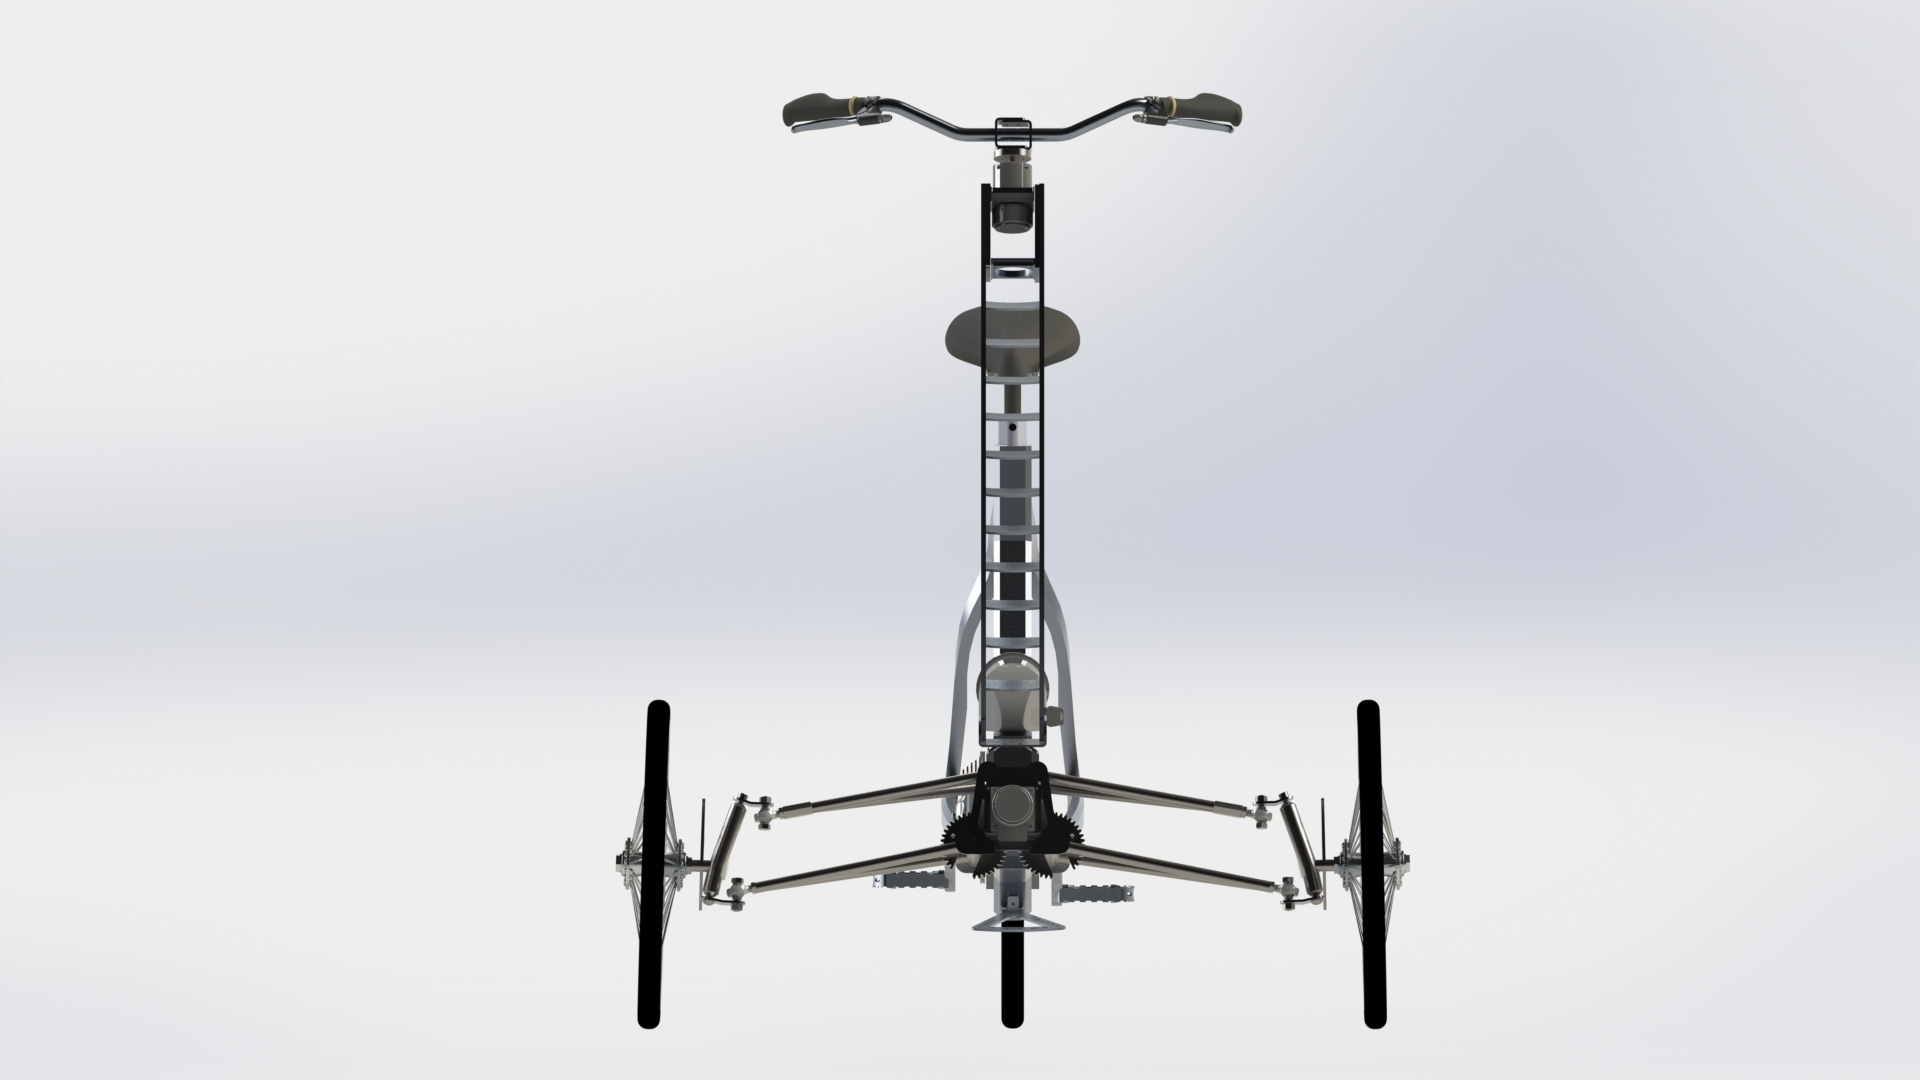
\includegraphics[width=1.15\linewidth]{figs/05/Render_Design_B_6}
	\caption{Front render}
	\\[-1cm]
\end{figure}

\newpage
\begin{figure*}[h!]
	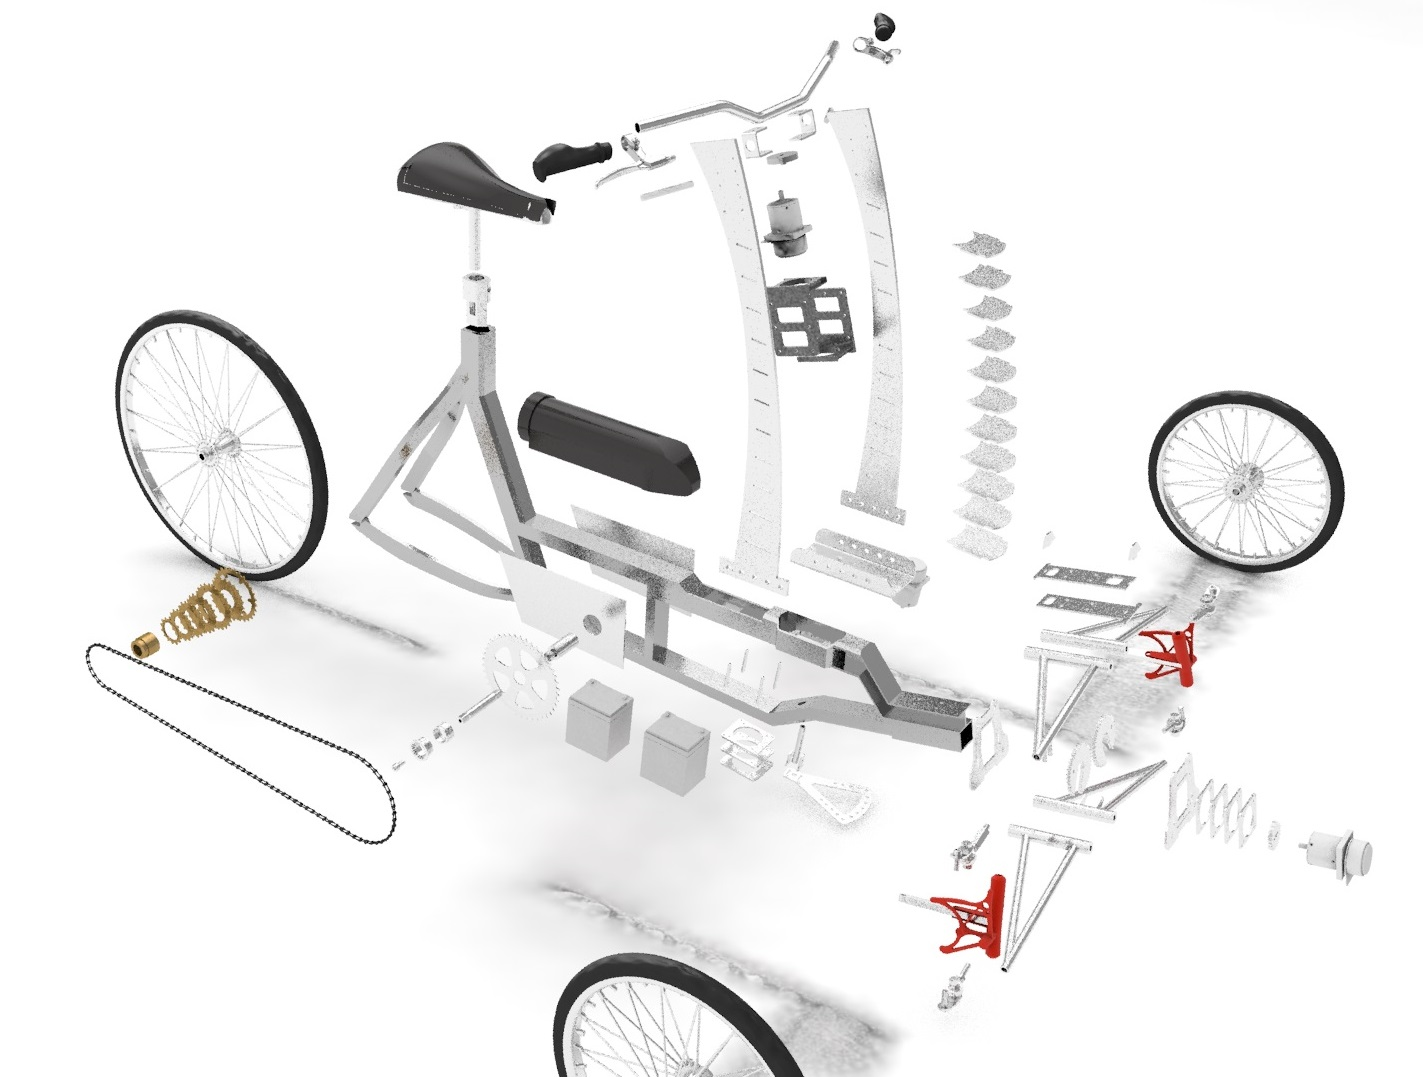
\includegraphics[width=0.9\linewidth]{figs/05/CreamBox0150}
	\caption{PEV components explosion}
\end{figure*}
$ $
\begin{figure*}[h!]
	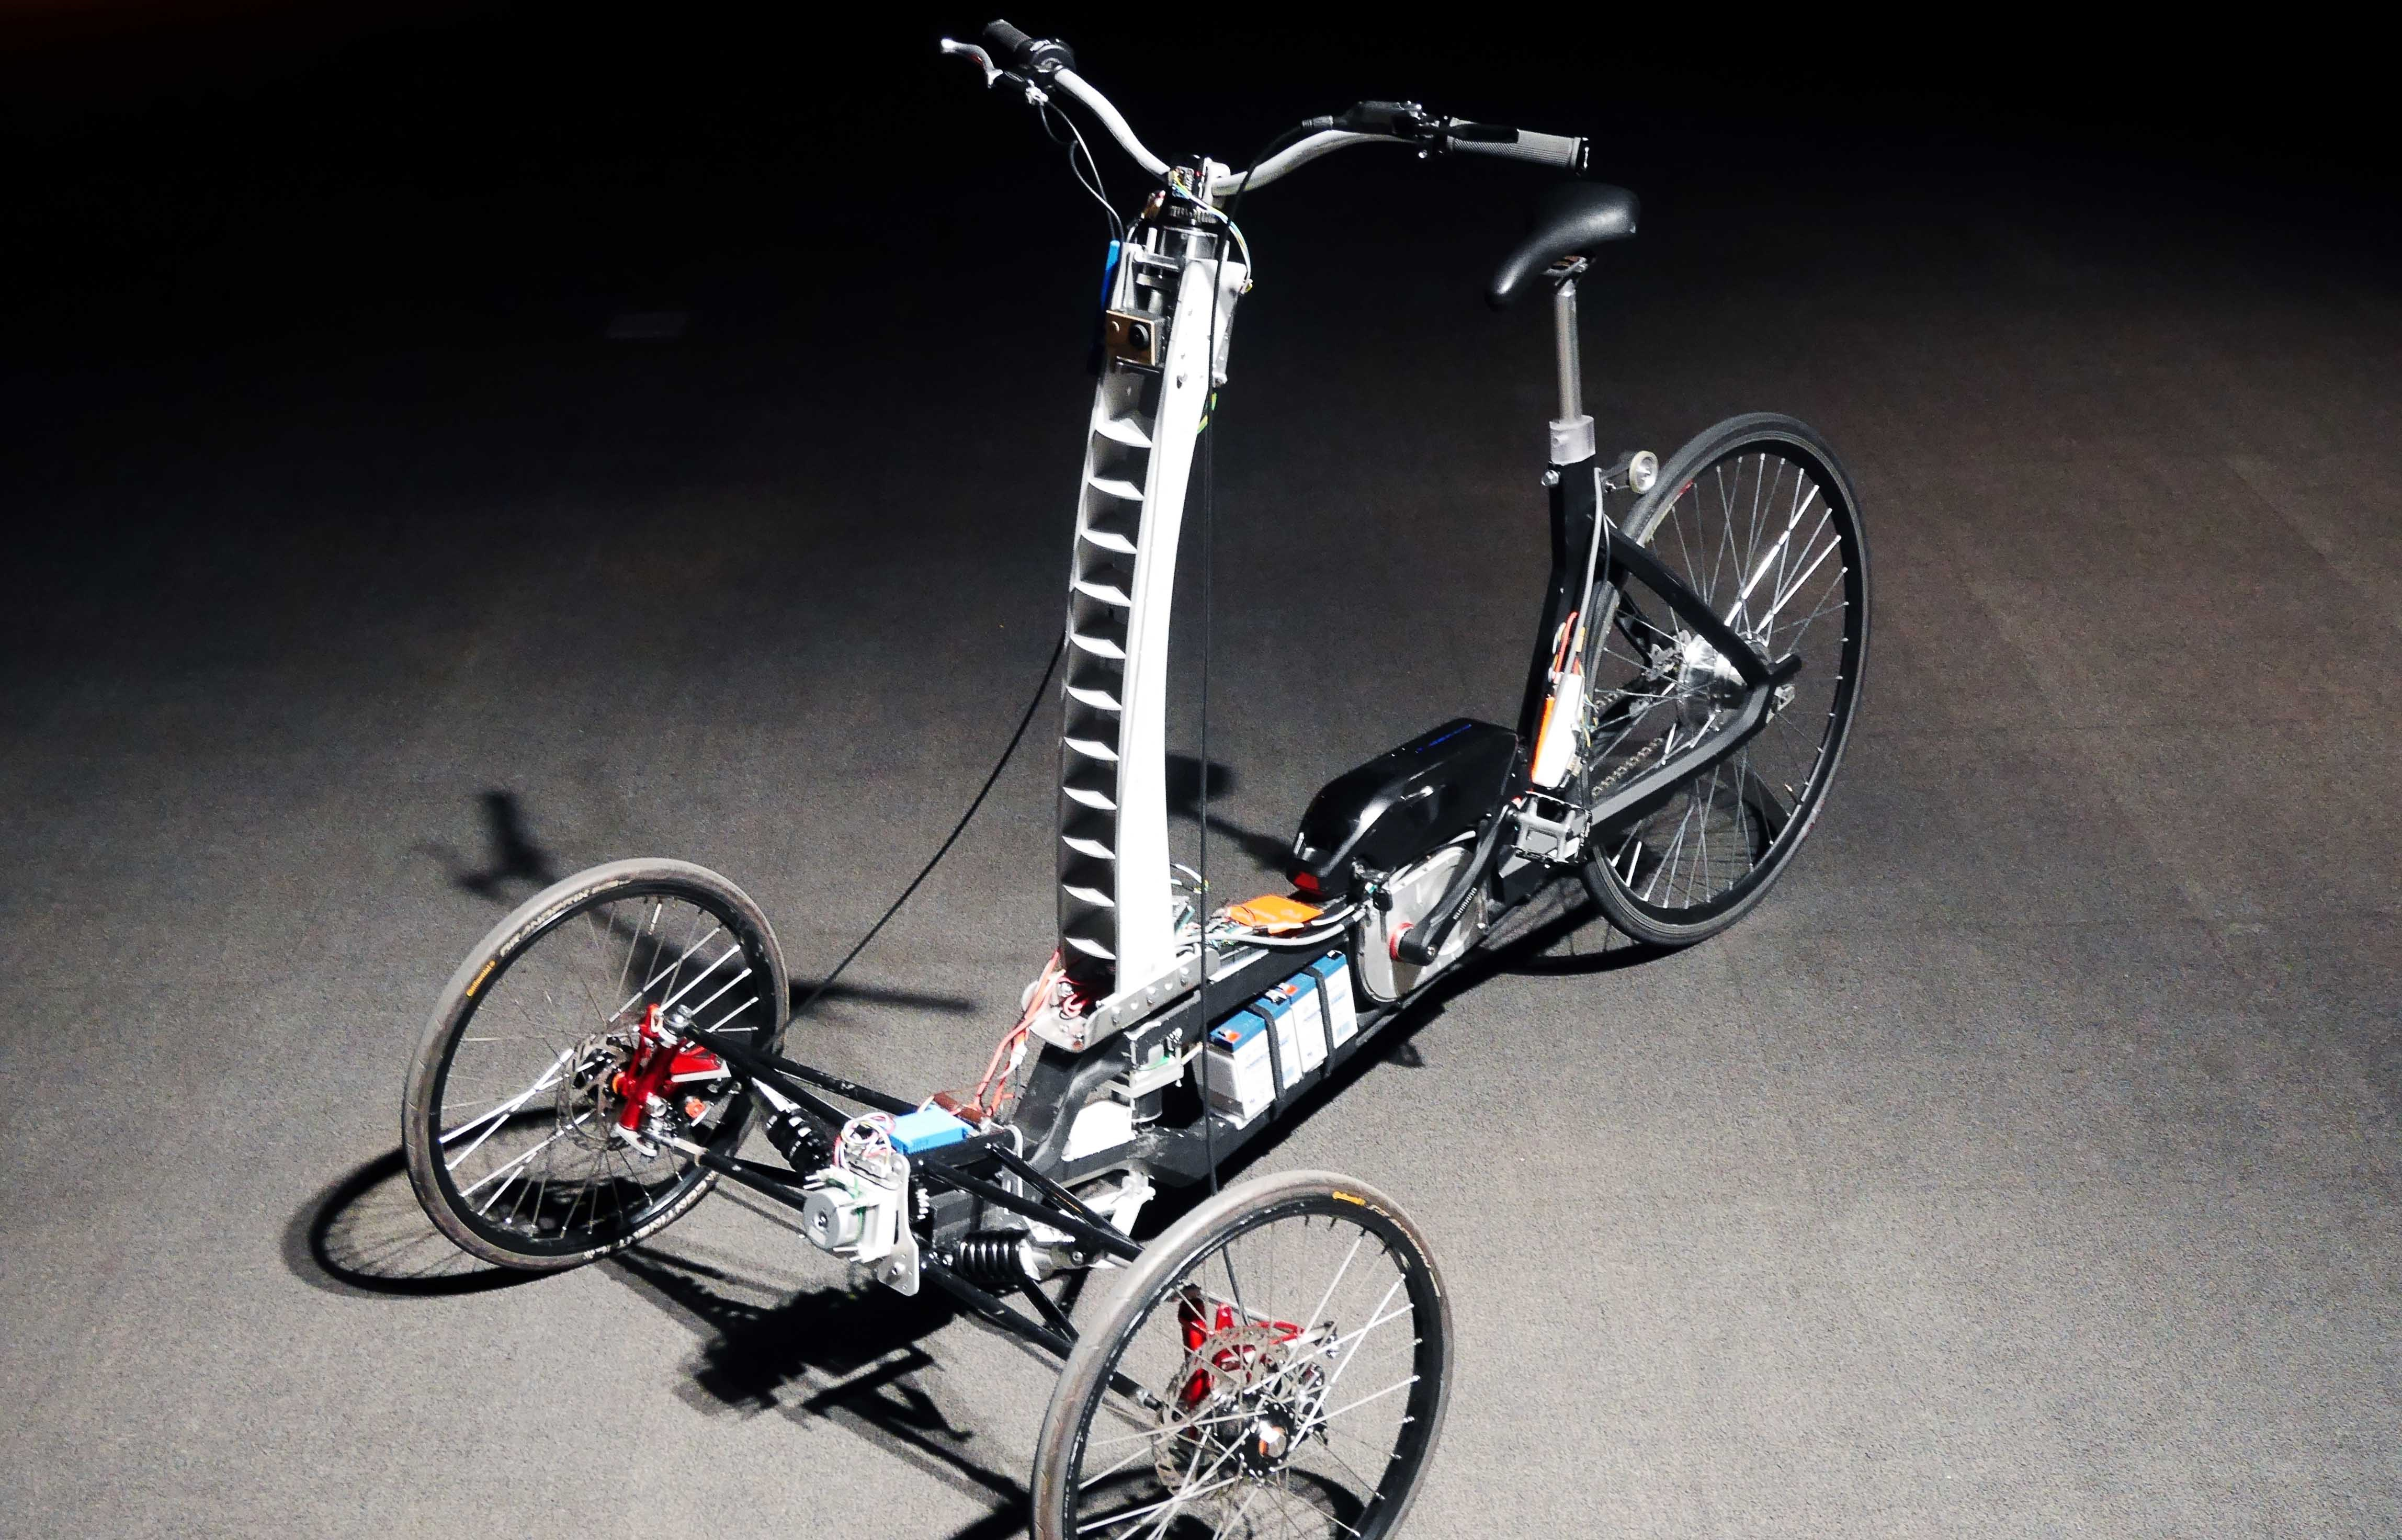
\includegraphics[width=0.95\linewidth]{figs/05/P10507152}
	\caption{PEV}
\end{figure*}

%\begin{figure}[h!]
%	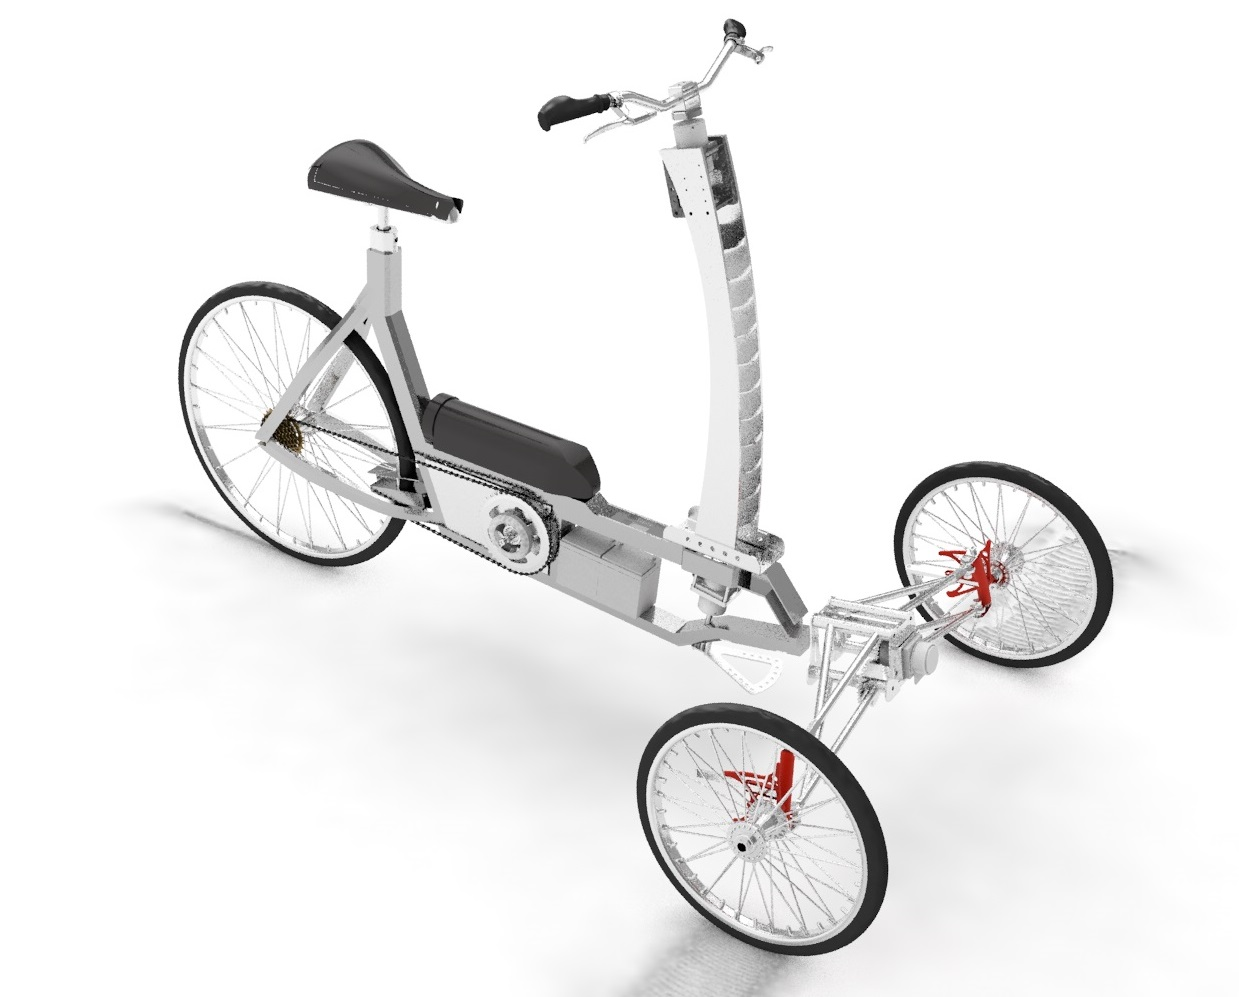
\includegraphics[width=1\linewidth]{figs/05/CreamBox0210}
%	\caption{Render}
%	\\[-1.5cm]
%\end{figure}
%\begin{figure}[h!]
%	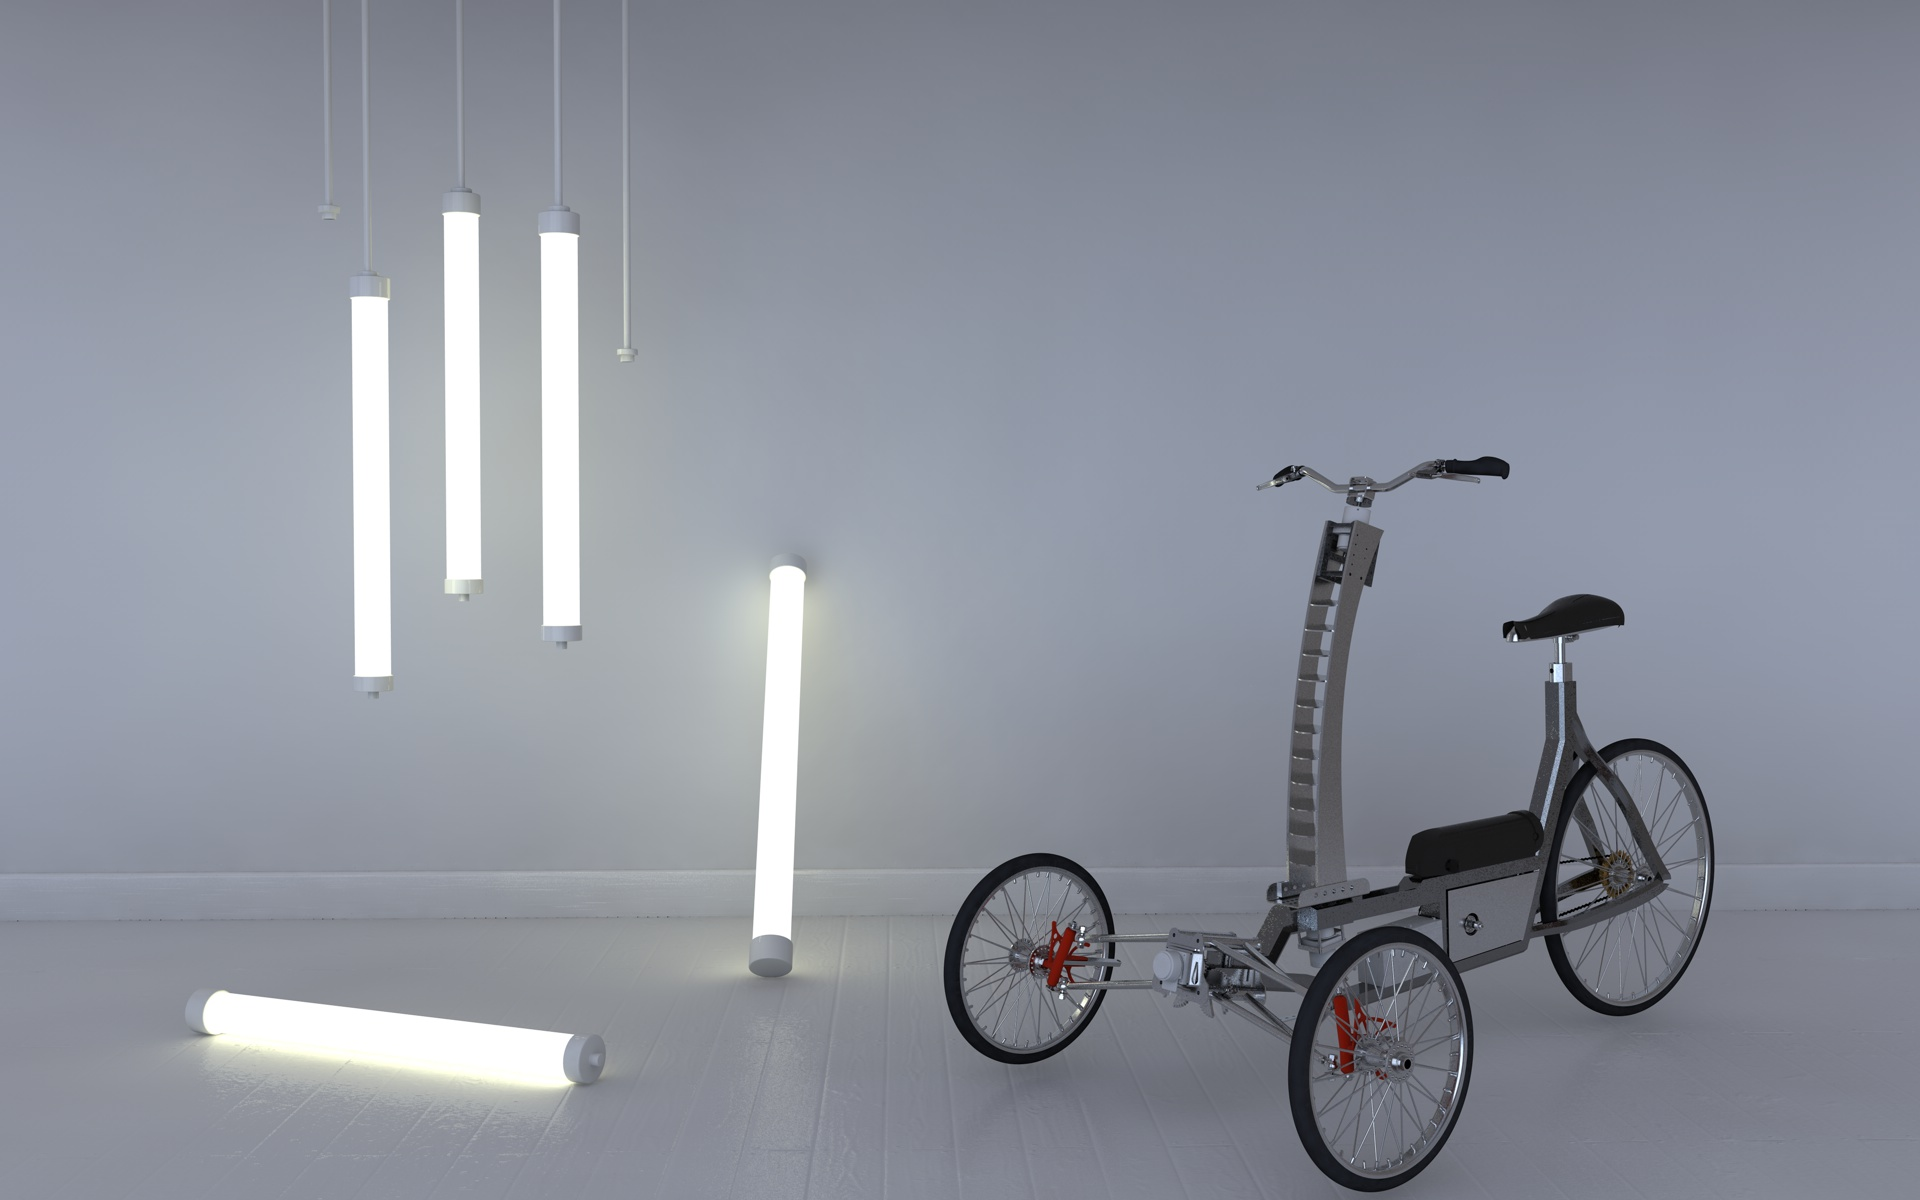
\includegraphics[width=1\linewidth]{figs/05/QuietRoom5}
%	\caption{Render}
%	\\[-1.5cm]
%\end{figure}



\newpage
\section{Electronics}
Electronics lay the foundation for a mechatronical project. In this section the used components are presented and the process to implement them correctly in the PEV is explained.
\subsection{PID Control}
Before using the VESC controller --open source, highly modifiable electronic speed controller ESC by Benjamin Vedder--, a NIDEC driver was used to control the angular position of the tilting motor. This happened in an early stage part of the project, so that the PEV final version was designed with VESC controllers.

The driver had 4 pins to control the motor:
\begin{itemize}
\begin{itemize}
	\item \textbf{PWM}: Pulse width modulation signal, it determines the speed of the motor. It is considered as a integer between 0 and 255. The higher PWM, the faster the motor rotates. Connected to a PWM digital output pin in Arduino.
	\item \textbf{CCW}: Binary variable to select the direction of rotation (clockwise or counter clockwise). Connected to a digital pin.
	\item \textbf{FG}: Frequency Generator, it outputs a signal with a frequency proportional to the motor speed. The proportional constant was unknown, it was roughly estimated.
	\item \textbf{GND}: ground connected to the GND port in Arduino.
\end{itemize}
\end{itemize}

This driver was used to control the angular position of the tilting motor. The input to the motor will be the value of PWM, that will make the motor rotate at a certain speed. The speed will be read by the pulses coming through the FG pin. Since there are not position readings, the position will be calculated based on the speed and the frequency of the control. 

Before reviewing the control system in detail, it is important to make a distinction between the temporal and the Laplace domains. The control diagram represents the Laplacian domain, where the time variable $t$ is replaced by the complex variable (frequency $s$) by applying the Laplace transform. A variable in lowercase ($n$) will belong to the temporal domain, whereas a variable in uppercase ($N$) will belong to the Laplacian domain.

\newpage
\begin{figure*}[h!]
	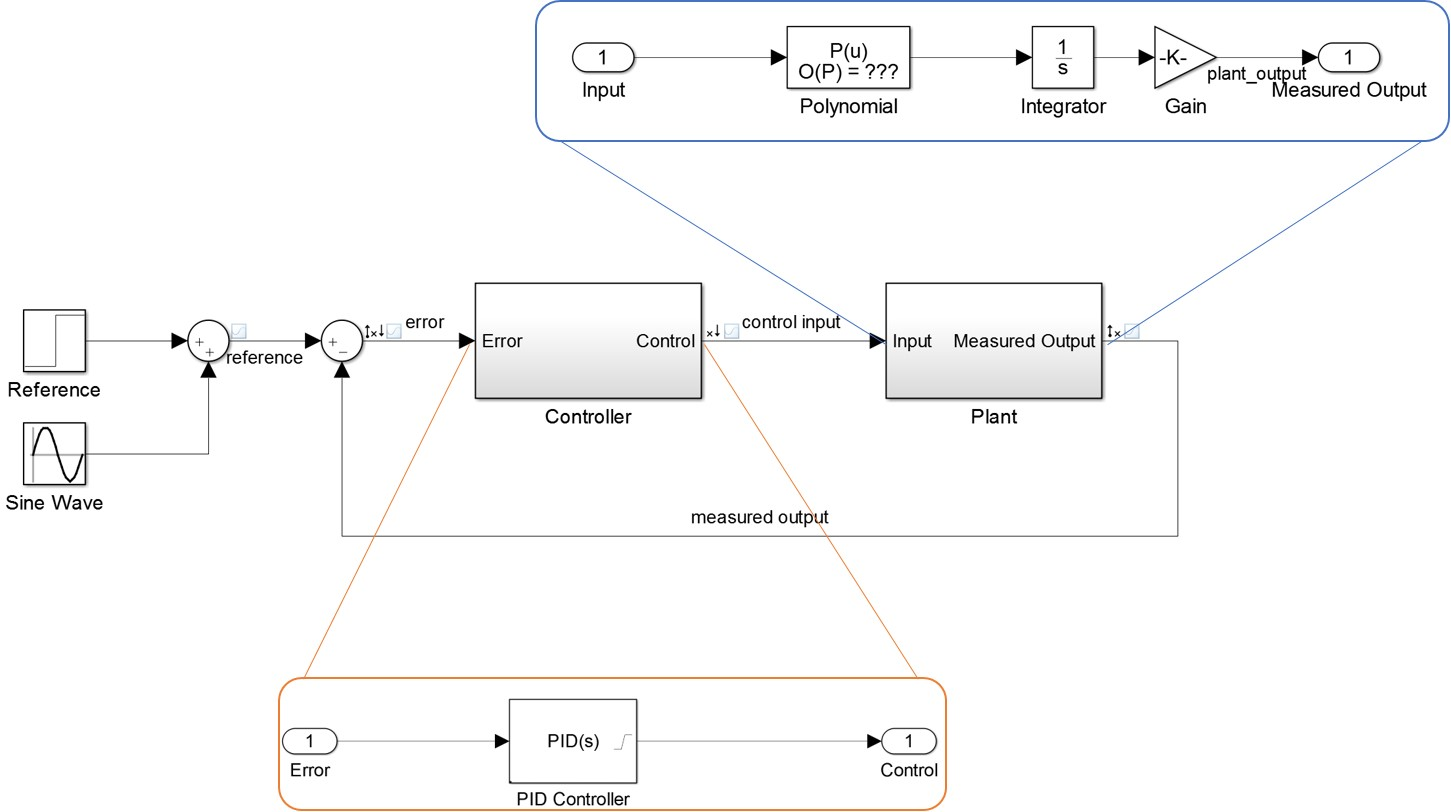
\includegraphics[width=1\linewidth]{figs/05/own/model_own_1}
	\caption{PID control of the angular position}
	\label{model_own_1}
\end{figure*}

The control diagram in Figure \ref{model_own_1} represents the inputs and outputs of this simple position control. The angular reference $\phi_{ref}$ is given by the user -- at first through a potentiometer-- and the error $e$ is calculated between the reference and the actual angle $\phi$. This error will be used to determine the input signal $pwm$ using a PID control. Finally, the $pwm$ will put an specific speed and therefore a position in that timestamp.
 
Translating these words into equations, the system equation is expressed as \[\phi_{i}=\phi_{i-1}+60n(t_{i}-t_{i-1})\] where $\phi_{i}$ is the angular position at time $t_{i}$ and $n$ is the speed in rpm.

The input variable $pwm$ is calculated from the error (defined as $E=\Phi_{ref}-\Phi$) by means of the PID control: 
\[pwm=K_{P}(\phi-\phi_{ref})+K_{I}\int_{t_{i-1}}^{t_{i}}(\phi-\phi_{ref}) dt + K_{D}\frac{\partial (\phi-\phi_{ref})}{\partial t}\] In the Laplacian domain: \[PWM=(K_{P}+\frac{K_{I}}{s}+K_{D})(\Phi_{ref}-\Phi)\]

The speed is the time derivative of the position with respect to the time:
\[n =\frac{\delta\phi}{\delta t}\,\frac{1\,rev}{2\pi\,rad}\frac{60\s}{1\,min}\quad\rightarrow\quad N=s\,\Phi \frac{60}{2\pi}\]

\newpage
\begin{marginfigure}[0cm]
	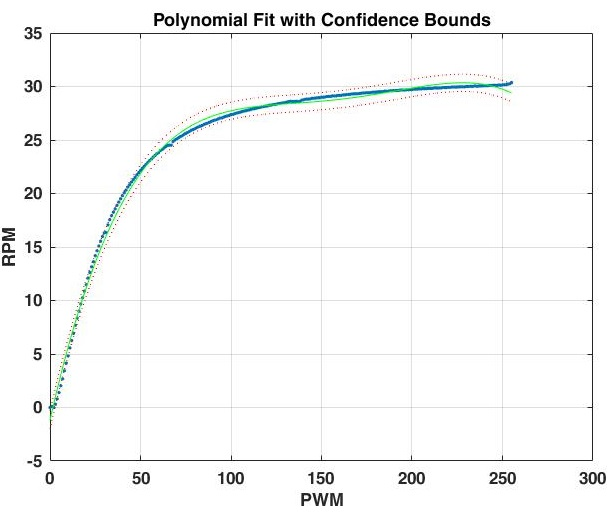
\includegraphics[width=1.2\linewidth]{figs/05/own/polynomial}
	\caption{Angular speed N vs signal PWM: Polynomial fitting}
	\label{polynomial}
\end{marginfigure}
\begin{marginfigure}[0cm]
	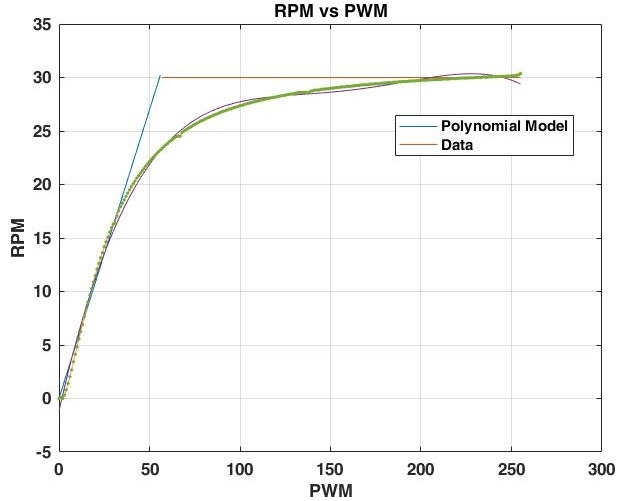
\includegraphics[width=1.2\linewidth]{figs/05/own/linear}
	\caption{Angular speed N vs signal PWM: Saturation and linear fitting}
	\label{linear}
\end{marginfigure}
The relation between the input $pwm$ and the output speed $n$ is not known, but it can be estimated. Using the speed information from the FG pin, some measurements were made to characterize the speed of the motor in function of the $pwm$ input. In Figure \ref{polynomial} the obtained data is represented and fitted into a 5th grade polynomial curve. \[N=f(PWM)\] In Figure \ref{linear}, on the contrary, the speed-pwm relation is simplified by a linear regression (the speed is saturated at $pwm=57$)
\[N=K\,\,PWM\]
Therefore, the speed is represented in function of the error:
\[N=s\,\Phi \frac{60}{2\pi}=f(PWM)=f\big((K_{P}+\frac{K_{I}}{s}+K_{D})(\Phi_{ref}-\Phi)\big)\]
For the sake of simplicity, the transfer function is indicated for the relation $N=K\,PWM$
\[\Phi=\Phi_{ref}\frac{K_{P}\,s+K_{I}+K_{D}\,s^2}{\frac{60s^2}{2\pi\,K}+K_{P}\,s+K_{I}+K_{D}\,s^2}\]
The control strategy was implemented in MATLAB and the PID tuner turned out to be really useful to determine the values of $K_{P}$, $K_{I}$ and $K_{D}$. Overall the quality of this \textbf{PID control was satisfactory}, but the VESC controller resulted easier to implement and besides it provided more feedback from the motor (electrical and mechanical variables).
\begin{figure}[h!]
	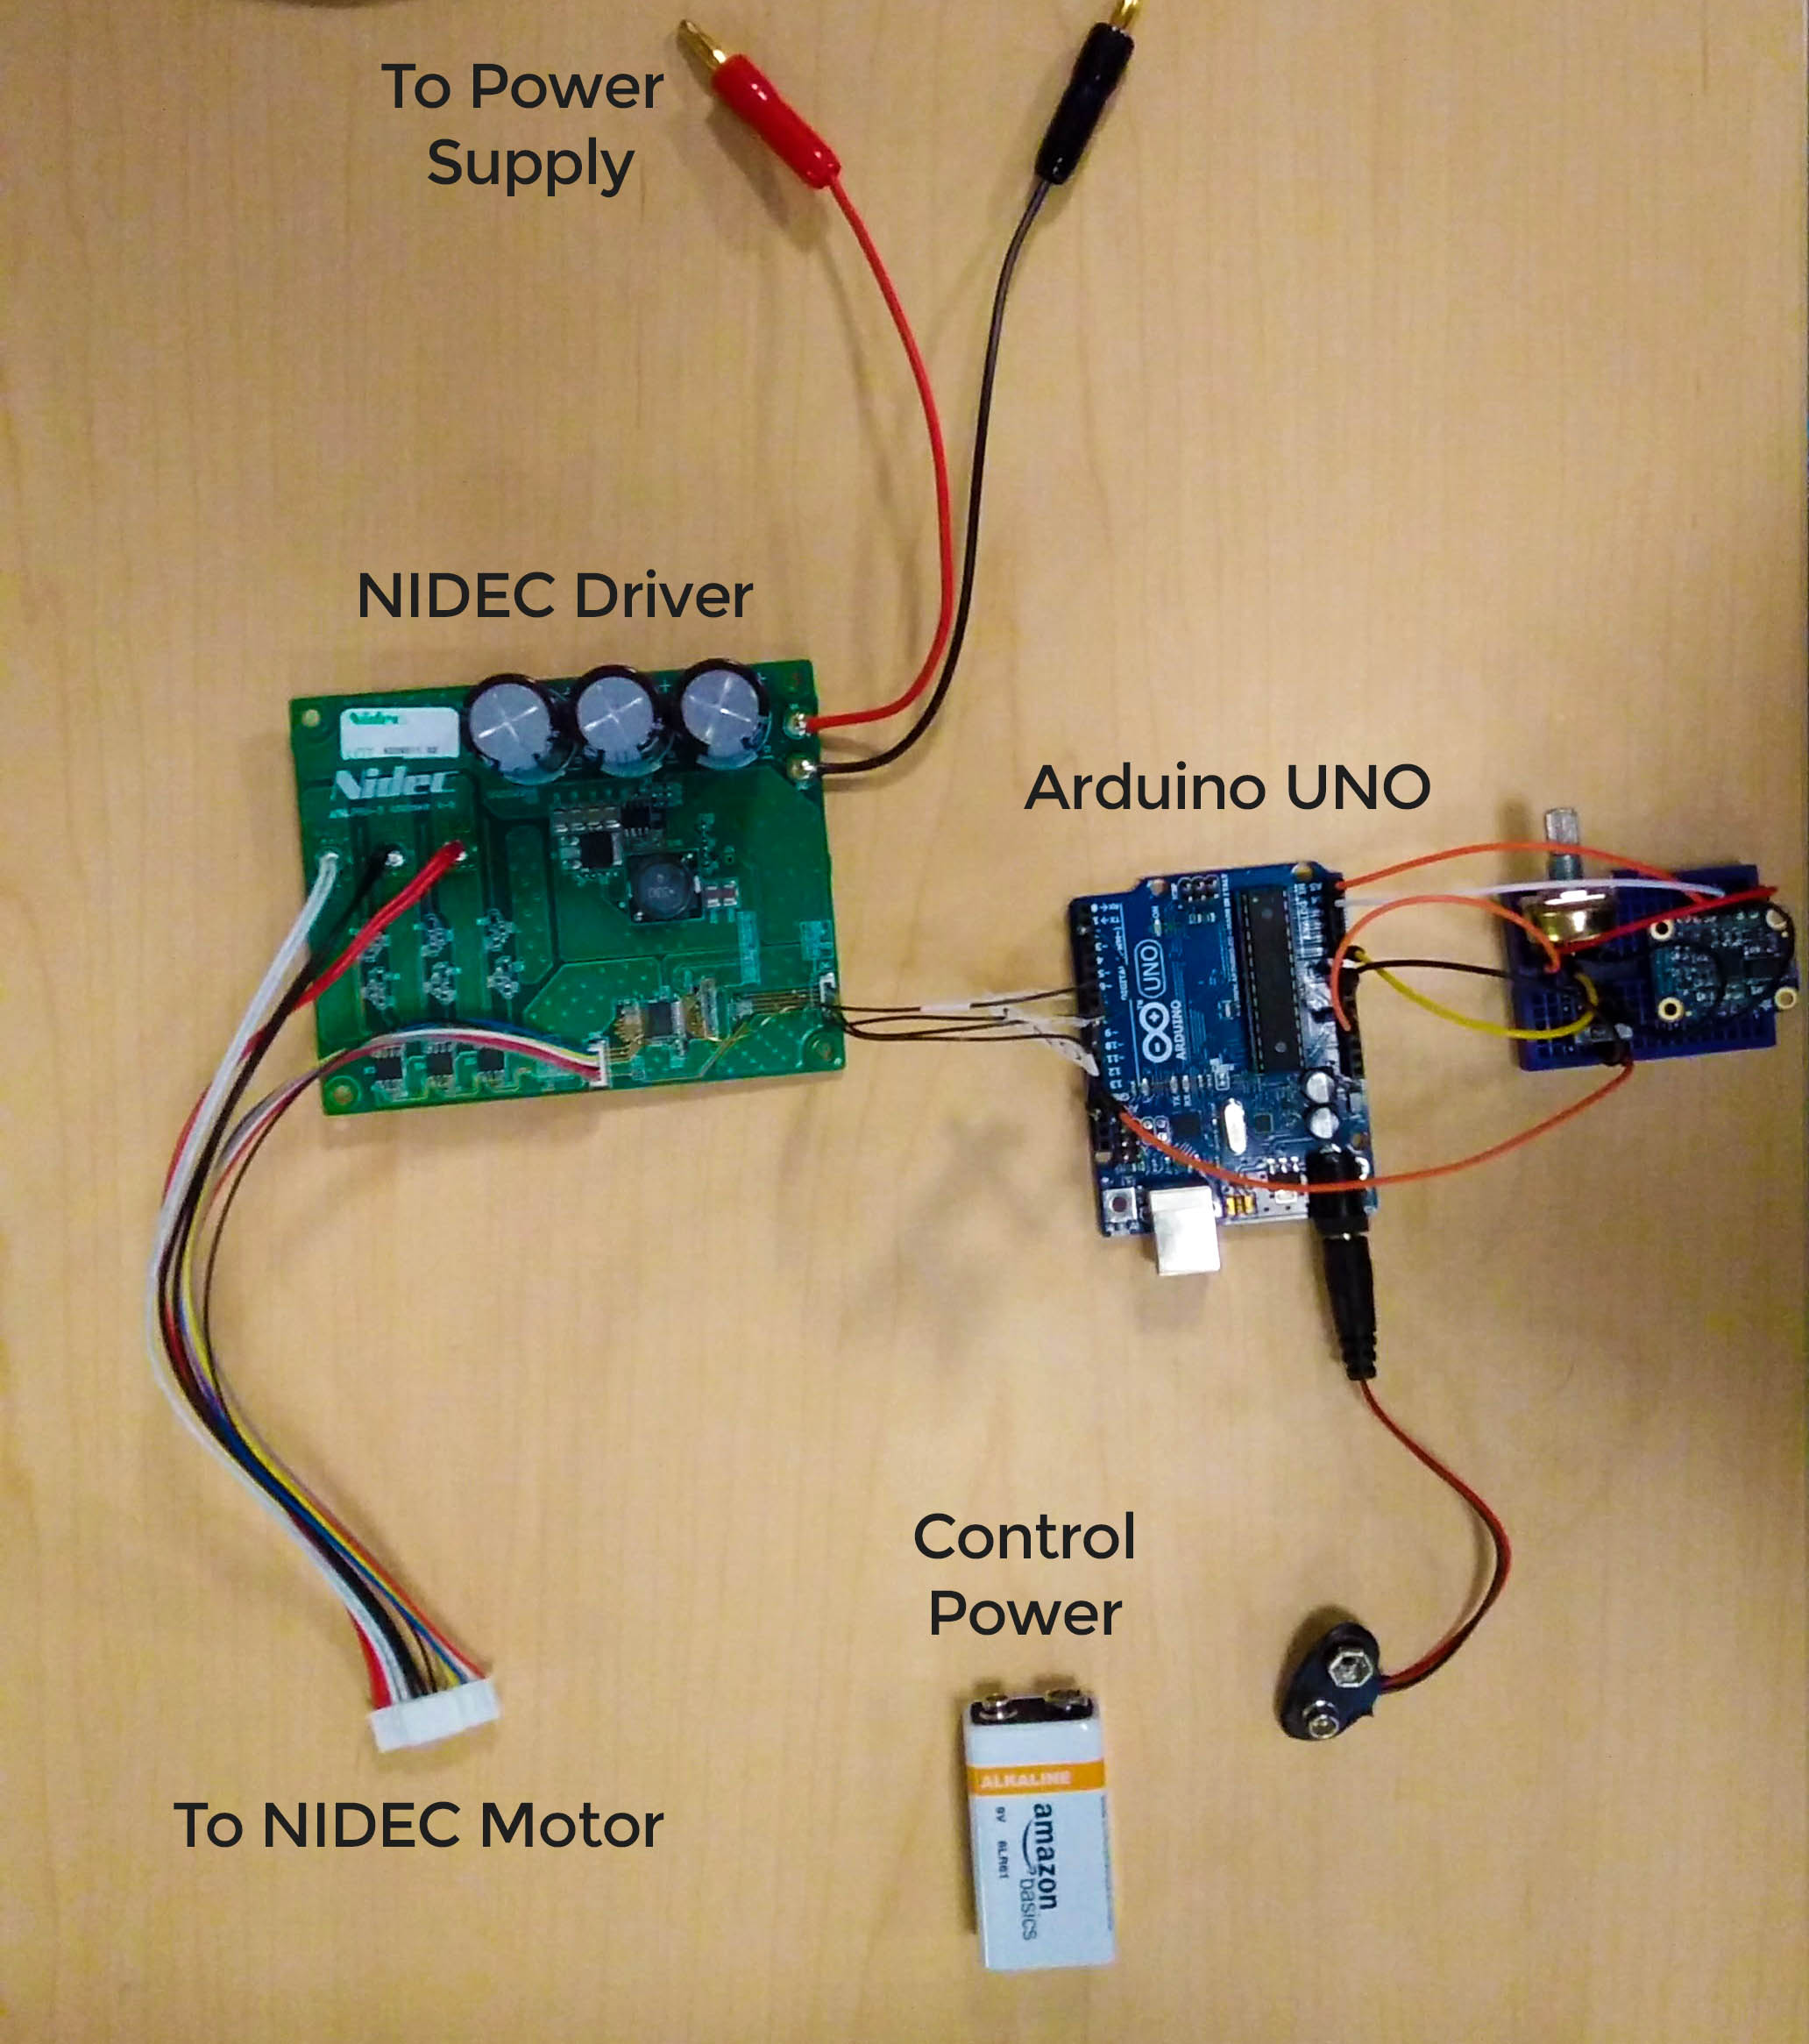
\includegraphics[width=0.85\linewidth]{figs/05/own/IMG_20161231_132543}
	\caption{Schematic of the early motor controller: Arduino UNO, 9V battery, potentiometer and NIDEC driver}
	\\[-10cm]
\end{figure}

\newpage
\subsection{VESC}

The VESC is a fully customizable open source electronic speed controller by Benjamin Vedder, designed for lightweight and compact applications like skateboards, or in this case, a three wheeler vehicle.

\begin{figure}[h!]
	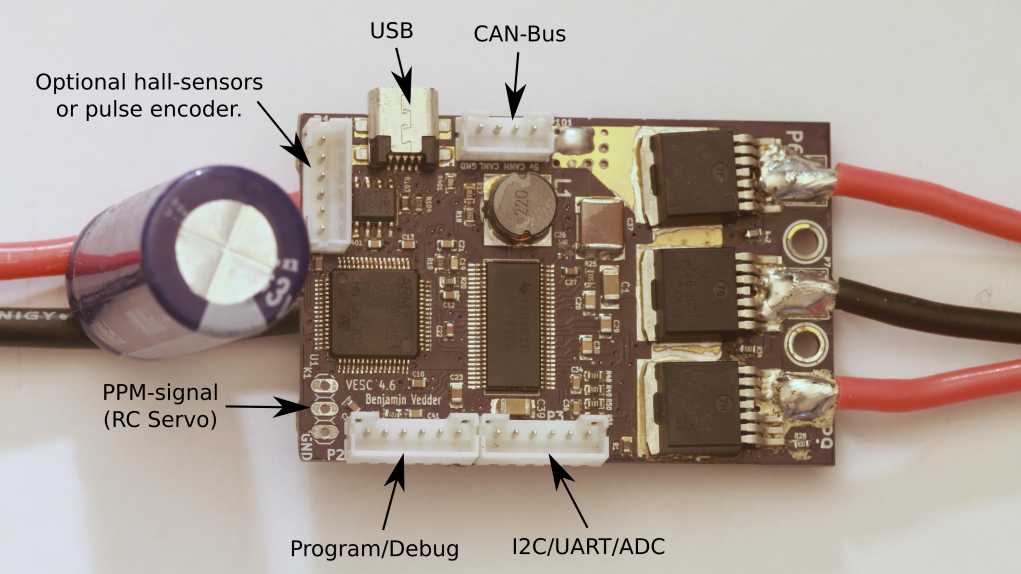
\includegraphics[width=1\linewidth]{figs/05/vesc}
	\caption{VESC Picture}
	\\[-1cm]
\end{figure}

The controller receives the power from the batteries and outputs the 3 phases $U$, $V$ and $W$ to the brushless motors. The incorporated firmware offers various possibilities to control the motor in different ways. Every motor in this PEV was configured to be controlled in FOC (Field Oriented Control) sensorless mode.

\textbf{FOC -- Field Oriented Control}

BLDC motors require a controller that converts the applied DC from the battery cells into AC to drive the motor. This task demands complex driving algorithms to commutate the coils in a sequence that achieves the desired directional rotation. A wide range of control algorithms are available:

\begin{itemize}
\begin{itemize}
	\item Trapezoidal control: For each of the 6 commutation steps, a pair of windings are powered, leaving the third disconnected. This method generates high torque ripple, leading to vibration, noise, and poor performance.
	
	\item Sinusoidal control: it supplies sinusoidal varying current to the 3 windings, thus reducing the torque ripple and offering a smooth rotation. However, these time-varying currents are controlled using basic PI regulators, which lead to poor performance at higher speeds.
	
	\item Field Oriented Control: the torque and the flux can be controlled independently and provides faster dynamic response. There is no torque ripple and smoother, accurate motor control can be achieved at low and high speeds.
\end{itemize}
\end{itemize}

\textbf{VESC Library}

\marginnote{
\begin{tabular}{c}
\textbf{bldcMeasure struct} \\[1.5pt] \hline \\[-1.5pt]
Average Motor Current        \\[1.5pt]
Average Input Current        \\[1.5pt]
Duty Cycle                   \\[1.5pt]
Motor RPM                    \\[1.5pt]
Input Voltage                \\[1.5pt]
Amperes Hours                \\[1.5pt]
Amperes Hours Charged        \\[1.5pt]
Tachometer                   \\[1.5pt]
Tachometer Absolute          \\[1.5pt] \hline
\end{tabular}
}

The VESC was connected to the Arduino MEGA board through serial connection (UART). To facilitate the control of the motor, the VescUartControl library was used in Arduino to interface over UART with the VESC. 

The margin table summarizes the available data from the VESC. In addition, it was possible to set the motor current, the brake current, the angular position, the duty cycle and the RPM of the motor.

\hspace{1cm}

\begin{lstlisting}[style=codedef]
@@bool VescUartGetValue(struct bldcMeasure& values, int num);@@
	
	%\textit{Sends a command to VESC and stores the returned data}%

	@@values@@(struct bldcMeasure&) -  bldcMeasure struct with received data
	@@num@@(int) - the serial port in use (0=Serial; 1=Serial1; 2=Serial2; 3=Serial3;)
	@@return@@(bool) - true if success

@@void VescUartSetCurrent(float current, int num);@@
	
	%\textit{Sends a command to VESC to control the motor current}%

	@@current@@(float) -  the current for the motor
	@@num@@(int) - the serial port in use (0=Serial; 1=Serial1; 2=Serial2; 3=Serial3;)

@@void VescUartSetCurrentBrake(float brakeCurrent, int num);@@
	
	%\textit{Sends a command to VESC to control the motor brake}%

	@@brakeCurrent@@(float) -  the current for the brake
	@@num@@(int) - the serial port in use (0=Serial; 1=Serial1; 2=Serial2; 3=Serial3;)

@@void VescUartSetPosition(float position, int num);@@
	
	%\textit{Sends a command to VESC to control the motor position}%

	@@position@@(float) - the position in degrees for the motor
	@@num@@(int) - the serial port in use (0=Serial; 1=Serial1; 2=Serial2; 3=Serial3;)

@@void VescUartSetDuty(float duty, int num);@@
	
	%\textit{Sends a command to VESC to control the motor duty cycle}%

	@@duty@@(float) - the duty cycle for the motor
	@@num@@(int) - the serial port in use (0=Serial; 1=Serial1; 2=Serial2; 3=Serial3;)

@@void VescUartSetRPM(float rpm, int num);@@
	
	%\textit{Sends a command to VESC to control the motor rotational speed}%

	@@rpm@@(float) - the revolutions per second for the motor
	@@num@@(int) - the serial port in use (0=Serial; 1=Serial1; 2=Serial2; 3=Serial3;)

\end{lstlisting}


\textbf{VESC Features}
\begin{marginfigure}
	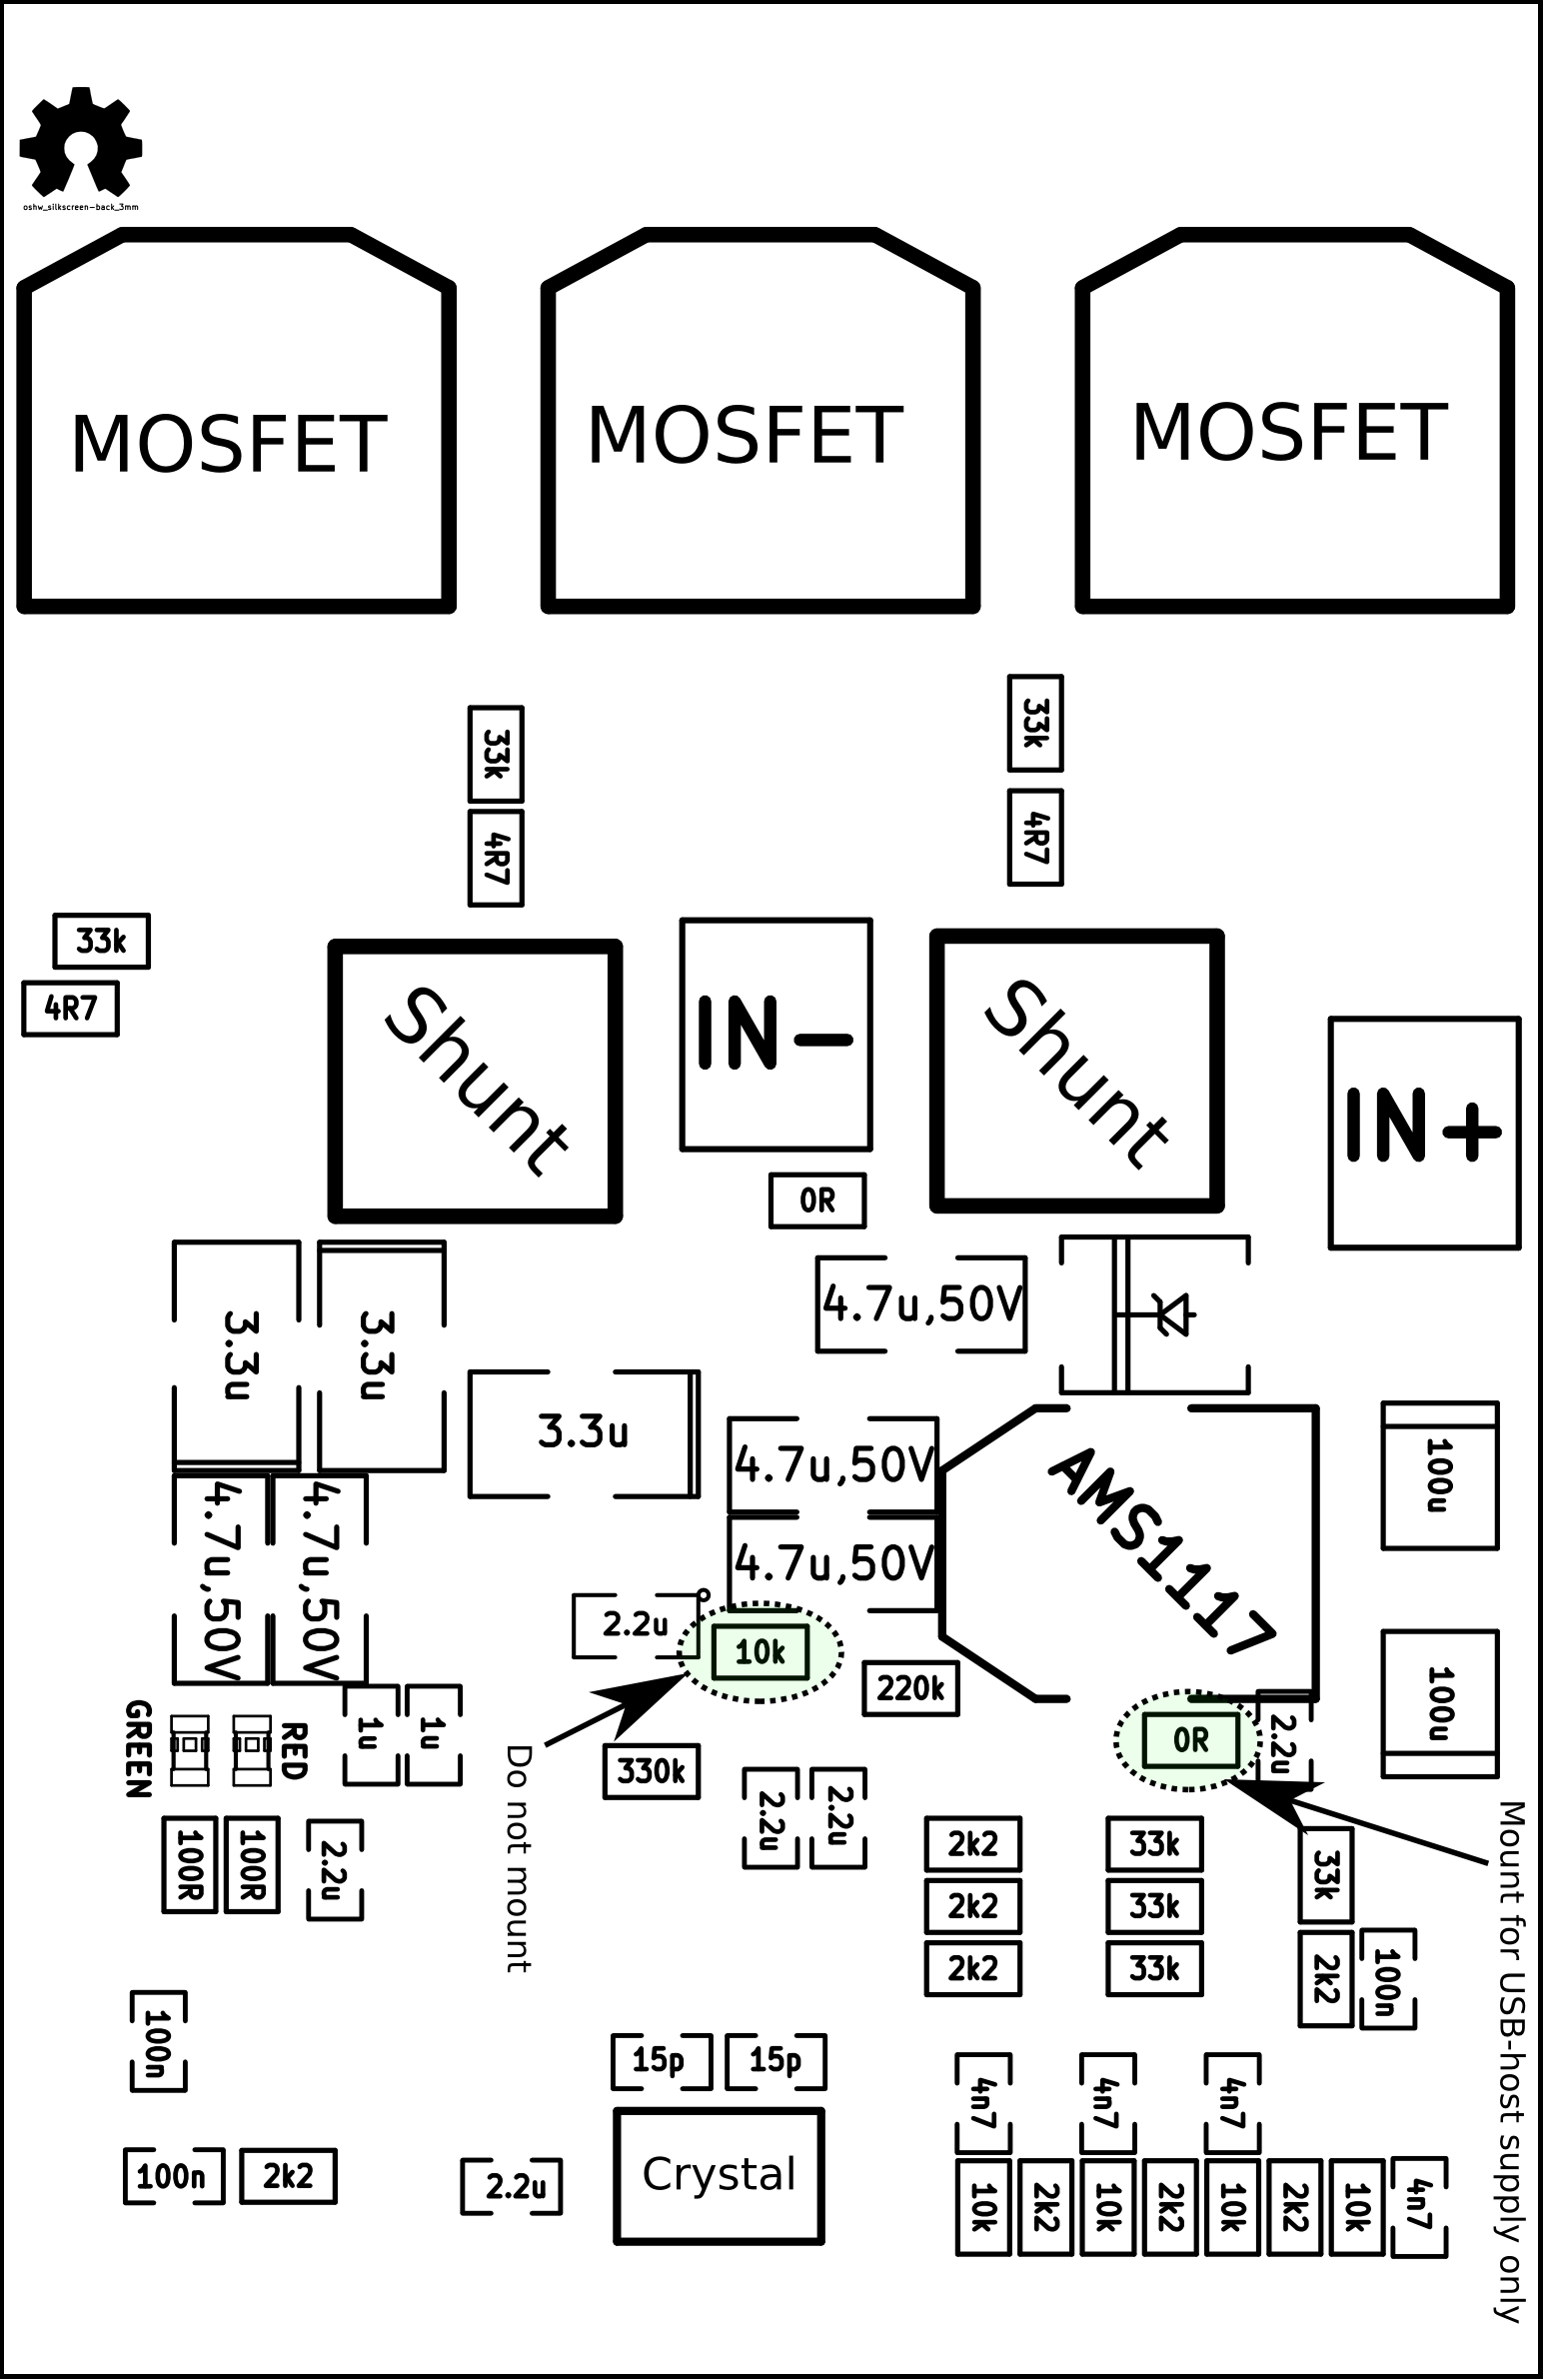
\includegraphics[width=0.65\linewidth]{figs/05/BLDC_41}
	\caption{Front VESC Schematic}
\end{marginfigure}
\begin{marginfigure}
	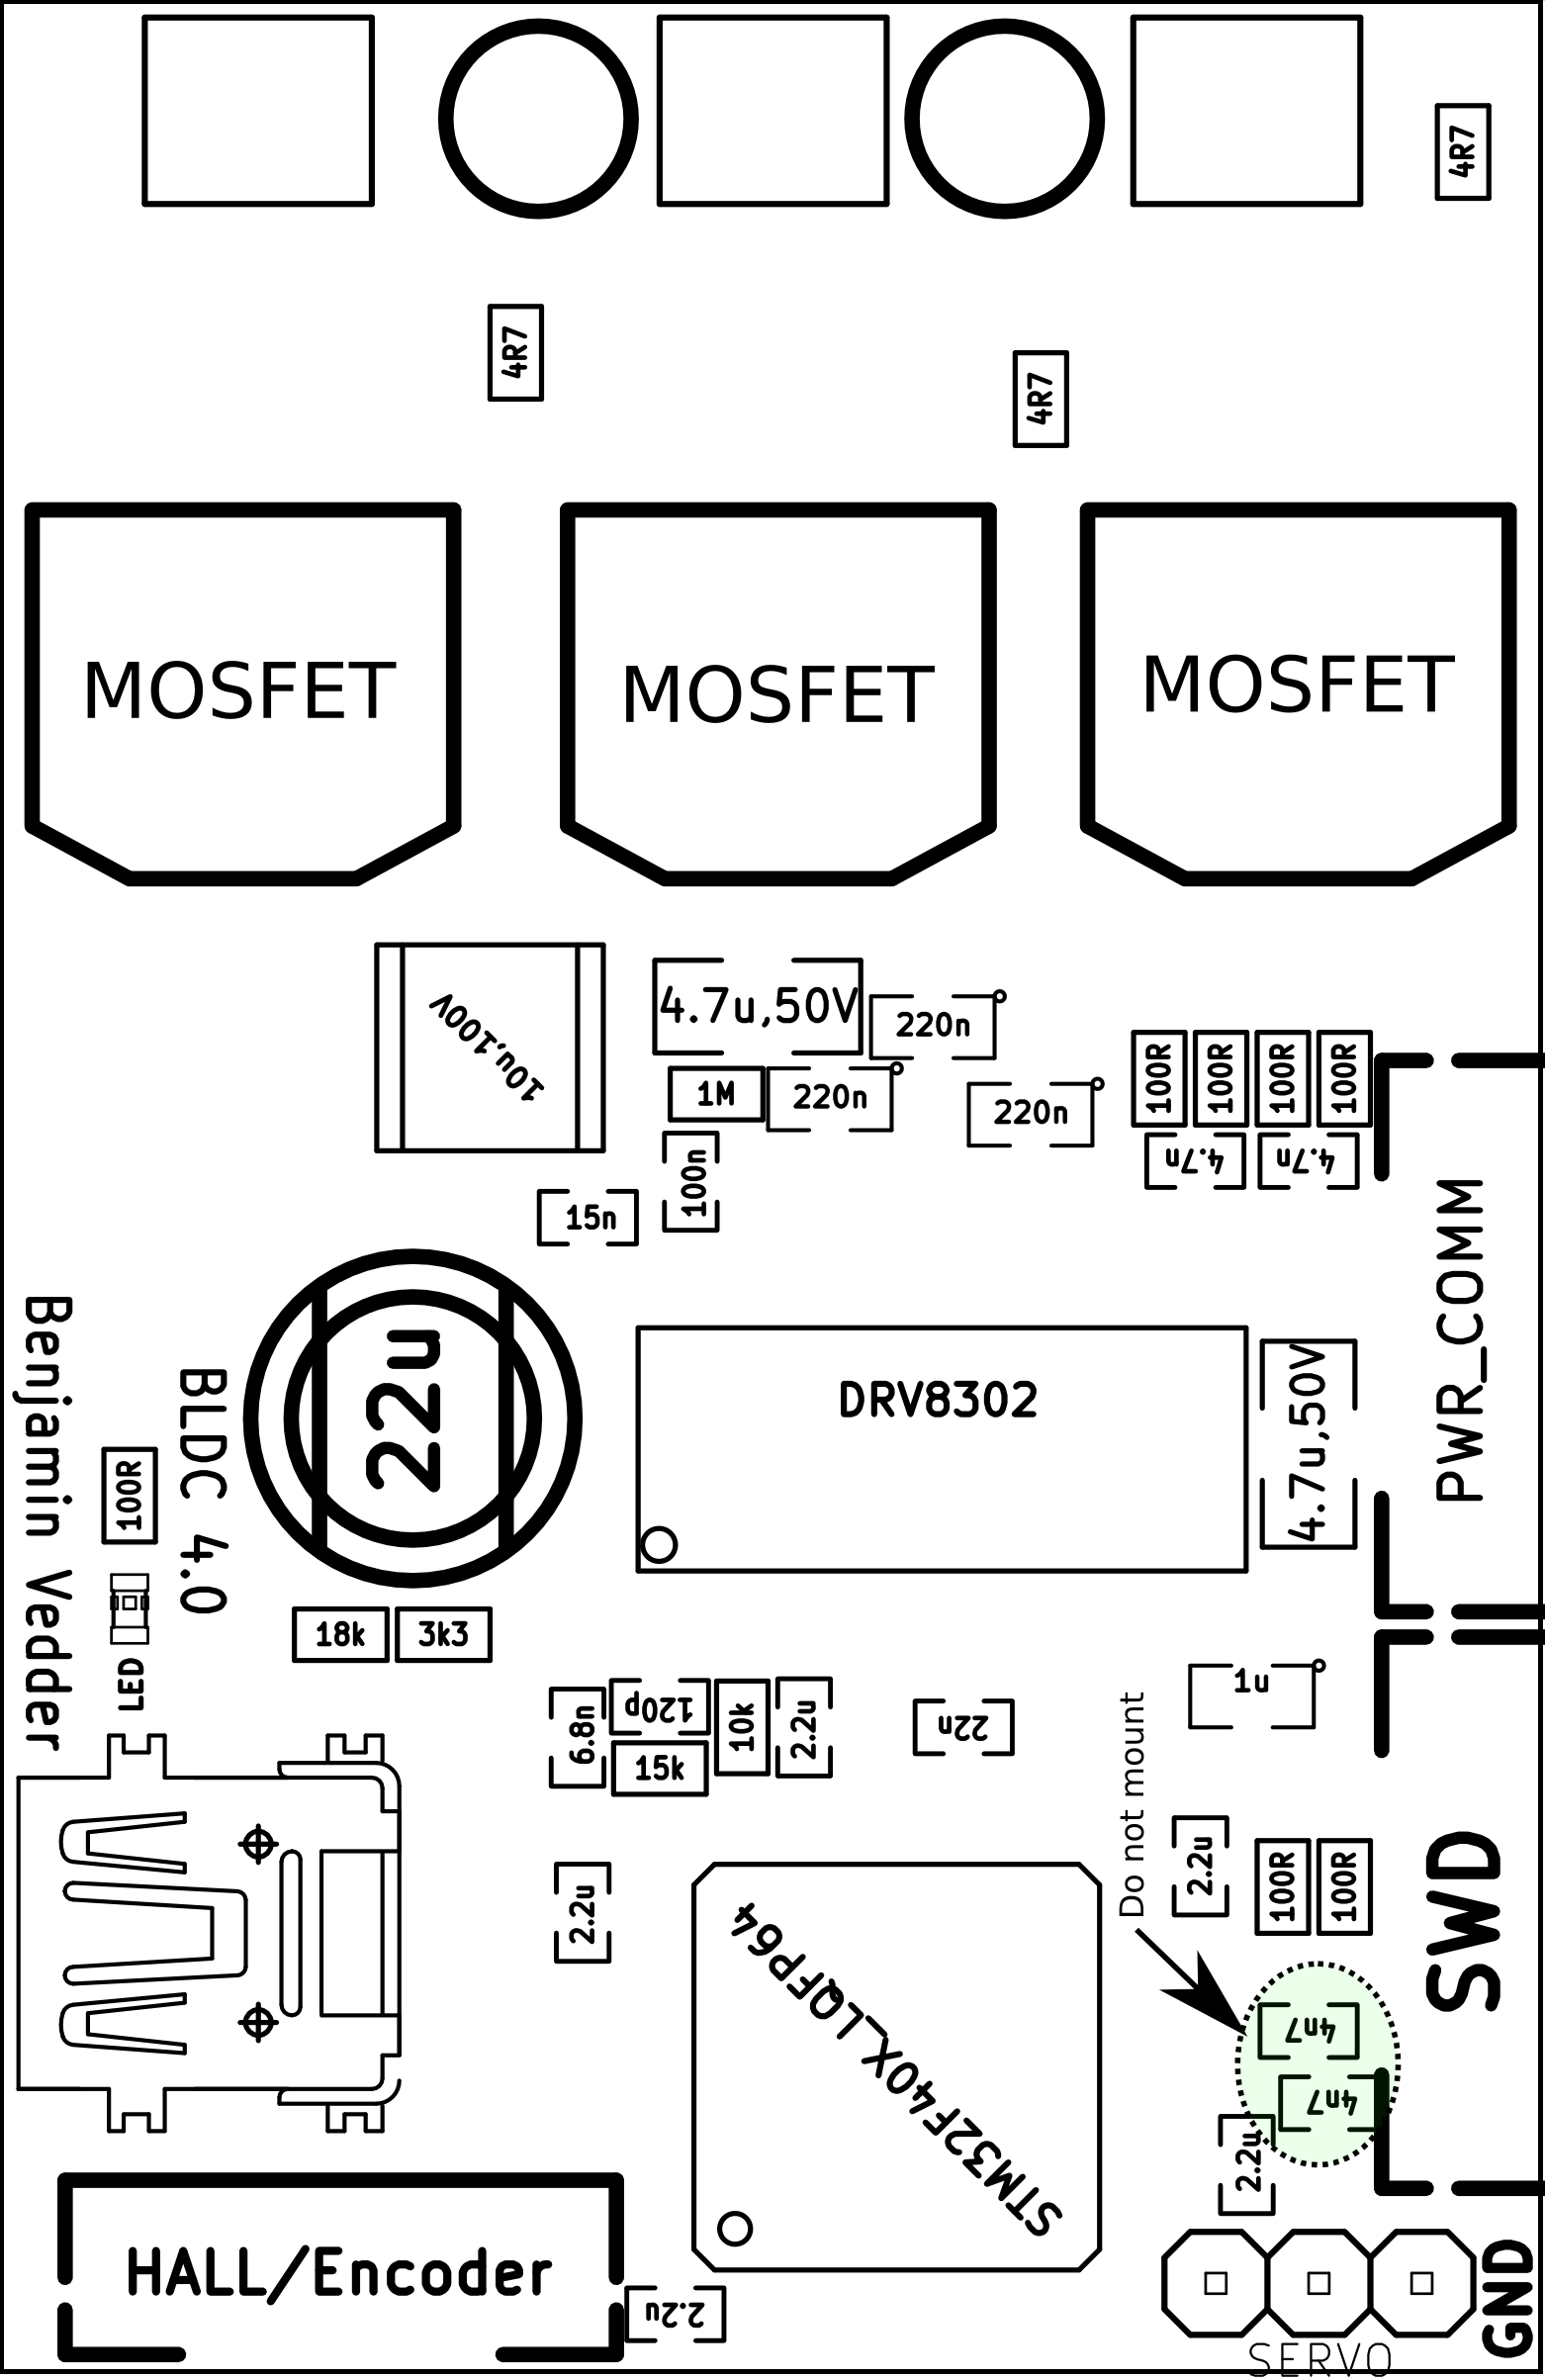
\includegraphics[width=0.65\linewidth]{figs/05/BLDC_42}
	\caption{Back VESC Schematic}
\end{marginfigure}
\begin{itemize}
\begin{itemize}\itemsep -10pt
\item Voltage $8V$ to $60V$
\item Current up to 240A for a some seconds or 50A continuous
\item 5V 1A output for external electronics (arduino)
\item Sensored and sensorless FOC, BLDC, and DC
\item Current and voltage measurement on all phases
\item Duty-cycle control, speed control or current control
\item Interface to control the motor: PPM signal, analog, UART, I2C, USB  or CAN-bus.
\item Regenerative braking
\item Good start-up torque in the sensorless mode
\item The motor is used as a tachometer, which is good for odometry
\item Adjustable protection against low/high input voltage and high motor/input current.
\end{itemize}
\end{itemize}


It is possible to plot the currents in the BLDC tool, voltages and the duty cycle in real-time. This is useful when debugging how everything behaves. Some screenshots of the configuration GUI (BLDC Tool):
\begin{figure}[h!]
	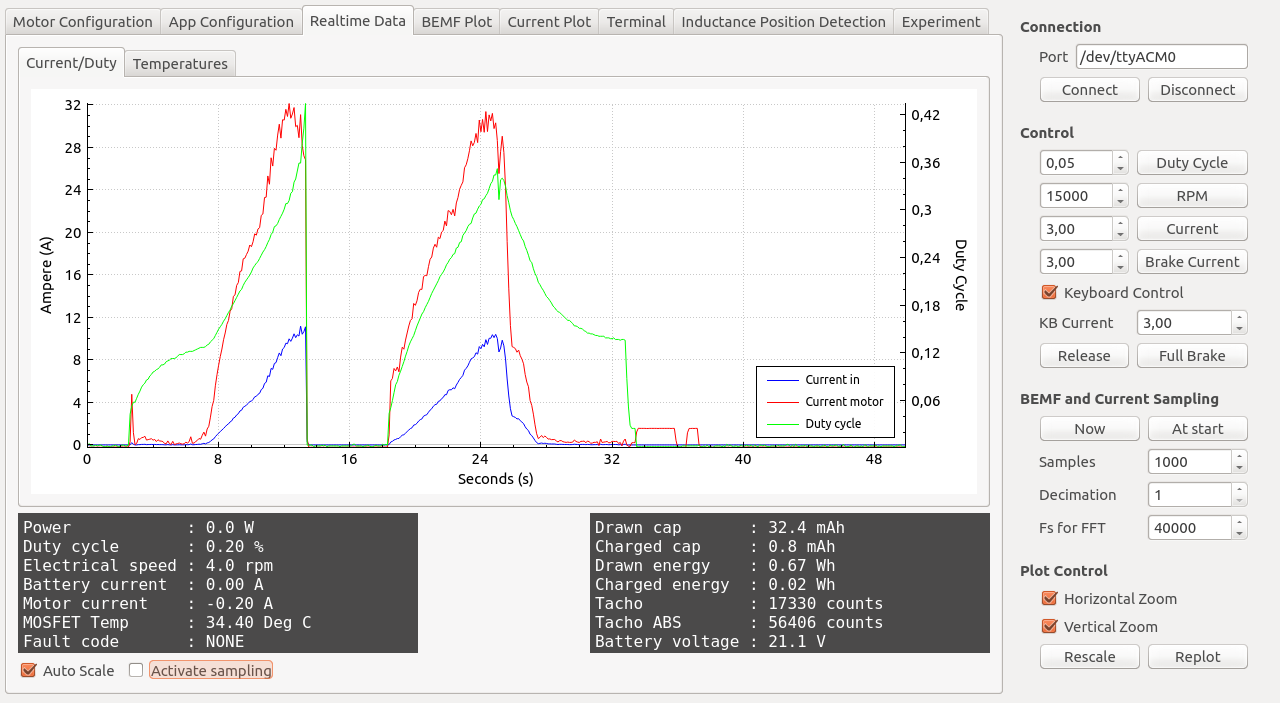
\includegraphics[width=1\linewidth]{figs/05/RT_Data}
	\caption{BLDC Tool}
\end{figure}

In order to protect the VESC from hazard and avoid any undesired contacts, some cases were 3D printed. The first version was designed to allocate only the board, whereas the second version had enough space to also incorporate the VESC capacitors.
\begin{marginfigure}[-4cm]
	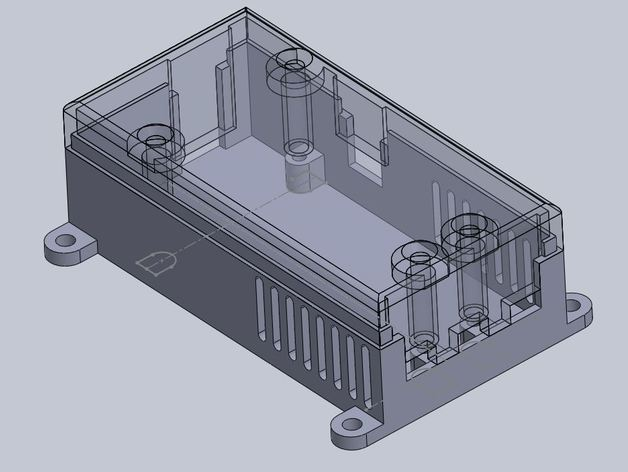
\includegraphics[width=0.9\linewidth]{figs/05/vesc_case_3}
	\caption{VESC case version 1}
\end{marginfigure}
\begin{marginfigure}
	\includegraphics[width=0.9\linewidth]{figs/05/vesc_case_6}
	\caption{VESC case version 2}
\end{marginfigure}

\newpage
\subsection{Rotary Encoder}

The longitudinal velocity of the PEV $V=V_{x}$ is obtained from a rotary encoder located in the rear wheel. This sensor is completely necessary, since the motor is not able to provide this information. The motor and the hub of the rear wheel are disentangled, meaning that the motor freely rotates inside the hub when the user pedals, for example. That is why the motor cannot give a feedback of the velocity of the wheel.

The rotary encoder or transmitter\cite{rotary} is a incremental optical encoder, that converts the motion to an electrical signal to indicate the position of the rear wheel. Transmitters must be used with a controller that has quadrature detection to get a 4X resolution increase and meet IP50 for protection from dust.

The code disk inside a quadrature encoder contains two tracks usually denoted Channel A and Channel B. These tracks or channels are coded ninety electrical degrees out of phase and this is the key design element that will provide the quadrature encoder its functionality. In applications where direction sensing is required, a controller can determine direction of movement based on the phase relationship between Channels A and B. As illustrated in the figure below, when the quadrature encoder is rotating in a clockwise direction its signal will show Channel A leading Channel B, and the reverse will happen when the quadrature encoder rotates counterclockwise.

\begin{marginfigure}
	\includegraphics[width=1\linewidth]{figs/05/encoder}
	\caption{Quadrature Encoder}
\end{marginfigure}

The resolution of this particular encoder is of 1000 counts per revolution. It has a 1.91"=48.5 mm diameter circumference polyurethane wheel attached to the shaft of the encoder. To get the speed of the PEV, a simple kinematic study was done, following the diagram in Figure \ref{encoder_2}:
\[\vec{v}_{0}=0 \quad \vec{v}_{A}=V\,\vec{i}=w_{1}\,R_{1}\,\vec{i} \quad \vec{v}_{P}=\vec{v}_{A}+w_{1}\,R_{1}\]
\[\vec{v}_{B}=V\,\vec{i}=w_{2}\,R_{2} \quad \vec{v}_{P}=\vec{v}_{B}+w_{2}\,R_{2}\]
Equaling the expression for the P point velocity $\vec{P}$:  
\[\vec{v}_{A}+w_{1}\,R_{1}=\vec{v}_{B}+w_{2}\,R_{2}\]
Since the velocities in the centers of both solid is the same ($\vec{v}_{A}=\vec{v}_{B})$):
\[w_{1}\,R_{1}=w_{2}\,R_{2}\] and therefore, \[V\,\vec{i}=w_{1}\,R_{1}=w_{2}\,R_{2}\]
For calculating the speed of the vehicle, the angular velocity and the radius of the small circumference attached to the encoder is only needed.

\begin{marginfigure}[-5cm]
	\includegraphics[width=1.15\linewidth]{figs/05/encoder_2}
	\caption{Wheel -- Encoder diagram}
\end{marginfigure}

The radius is known, and the angular velocity can be defined as:
\[w_{2}=\frac{\Delta\phi}{\Delta t}; \quad \Delta\phi=N_{counts}·\frac{1\,rev}{1000\,counts}·\frac{2\pi\,rad}{1\rev}\]
The speed is therefore calculated as:
\[V=N_{counts}·\frac{2\pi R_{1}}{1000\Delta t}\]
Every time that the encoder sends a pulse to the board, an interrupt routine starts to read that pulse and catch the rising or falling edge on the input pin. Therefore, if the Arduino is not fast enough, interrupting the microprocessor in the board can deny the reading of other pulses and considerably delay other operations. 

Taking into account that the resolution was really high (1000 counts/rev), and a radius of the encoder was 48.5/2=24.25 mm if the PEV is going at $1m/s$, for example, that means that in 1 second, the Arduino board needs to be able to interrupt its code more than 6500 times (6500 Hz). Increasing the speed of the vehicle increases this frequency as well.

To get the number of counts in a given time interval, it was necessary to implement a very fast digital reader in the Arduino Mega in order to not lose any count and estimate correctly the speed of the vehicle. 

In addition, this strategy works even better if a bit of hardware debouncing is forced on the rotary encoder. With two 0.1 uF capacitors soldered to the encoder pins, the number of calls to the interrupt routine is dramatically reduced. This is important because too many calls to the interrupt routine will rob computing cycles from the main routine, negating the effects of using interrupts to save computing power.
\begin{figure}[h!]
	\includegraphics[width=1\linewidth]{figs/05/P1050728}
	\caption{Rotary encoder mounted on the PEV}
	\\[-2cm]
\end{figure}

\newpage
\subsection{IMU}

\begin{marginfigure}[1cm]
	\includegraphics[width=1\linewidth]{figs/05/bno055}
	\caption{Bosch BNO055 9DOF IMU}
\end{marginfigure}
The selected inertial motion unit was the Bosch BNO055, a 9-axis absolute orientation sensor with sensor fusion. The BNO055 integrates a triaxial 14-bit accelerometer, a triaxial 16-bit gyroscope with a range of 2000 degrees per second, a triaxial geomagnetic sensor and a 32-bit microcontroller.

It is connected through I2C (clock and data pins) to the analog pins in the Arduino. The PEV is equipped with a pair of BNO055, both connected through I2C, with the difference that the second IMU's ADC pin is connected to the board as well. Setting the ADR pin to high changes the I2C address from the default (0x28 to 0x29).

\marginnote{VIN: 3.3-5.0V power supply input \\
GND: common for power and logic \\
SCL - I2C clock pin \\
SDA - I2C data pin \\
ADR: to change the I2C address \\
}

Rather than spending a lot of time with algorithms of varying accuracy and complexity, the data can be extracted very easily thanks to the sensor fusion. However, it requires to configure it properly when powered. 
\begin{enumerate}\itemsep -10pt
\item The operation mode has to be setup to be able to configure it (CONFIG MODE)
\item Limit accelerometer range to 2G, get better accuracy
\item Calibrate using some offsets values obtained previously
\item The operation mode is setup again to Fusion mode with NDOF, mode from which the absolute orientation can be obtained.
\end{enumerate}

\textbf{Calibration}

To obtain correct values from the IMU, it has to be properly calibrated first. Once the device is calibrated, the calibration data will be kept until the BNO is powered off. The BNO doesn't contain any internal EEPROM, so a new calibration will be needed every time the device starts up, or a manual restore of the calibration data.

The BNO055 includes internal algorithms to constantly calibrate the gyroscope, accelerometer and magnetometer. The four calibration registers -- an overall system calibration status, as well individual gyroscope, magnetometer and accelerometer values -- will return a value between '0' (uncalibrated data) and '3' (fully calibrated).

The sensors are trimmed to tight offsets, meaning valid data is obtained even before the calibration process is complete, but particularly in NDOF mode any data should be discard as long as the system calibration status is 0. The reason is that system cal '0' in NDOF mode means that the device has not yet found the north pole, and orientation values will be off. The heading will jump to an absolute value once the BNO finds magnetic north.

To generate valid calibration data, the following criteria should be met:
\begin{itemize}
\begin{itemize}\itemsep -10pt
\item Gyroscope: the device must be standing still in any position
\item Magnetometer: normal movement of the device is sufficient
\item Accelerometer: the BNO055 must be placed in 6 standing positions for +X, -X, +Y, -Y, +Z and -Z.
\end{itemize}
\end{itemize}

\textbf{Position of the IMU}

\begin{marginfigure}[0cm]
	\includegraphics[width=1.2\linewidth]{figs/05/IMU_Overall}
	\caption{Location of IMU A and B}
\end{marginfigure}
The PEV is equipped with a pair of IMUs, one placed on the handle bar and another one fixed on the frame. The justification for this decision lays on two arguments:
\begin{itemize}
\begin{itemize}
\item The relative angle between the frame and the handle bar can be obtained, meaning that an encoder is not needed in the handle bar.
\item The perceived lateral acceleration $a_{per}$ has to be obtained along the lateral axis $y'$, which should not be affected by the handle bar steering.
\item The steering angle $\delta$ and its rate $\dot{\delta}$ can be also obtained from the gyroscope
\end{itemize}
\end{itemize}

\textbf{Orientation of the IMU}

\begin{marginfigure}[5cm]
	\includegraphics[width=1.1\linewidth]{figs/05/Euler}
	\caption{Quaternion vector diagram}
\end{marginfigure}
Due to the fact that each IMU is oriented differently, it is necessary to process the orientation data depending on the case. The angular orientation from each IMU is obtained from the quaternion: \[\vec{q}=\begin{bmatrix} q_{w} \\ q_{x} \\ q_{y} \\ q_{z} \end{bmatrix}=\begin{bmatrix} \cos(\alpha/2) \\ \sin(\alpha/2)\cos(\beta_{x}) \\ \sin(\alpha/2)\cos(\beta_{y}) \\ \sin(\alpha/2)\cos(\beta_{z}) \end{bmatrix}\]
where $\alpha$ is a simple rotation angle and $\cos(\beta_{x})$, $\cos(\beta_{y})$ and $\cos(\beta_{z})$, are the direction cosines locating the axis of rotation.

The quaternion is then transformed into the appropriate Euler angles: Roll, Pitch and Yaw. Each of these angles is related to one of the axis X, Y and Z. Depending on the order of the rotations --XYZ and ZYX Euler angles are not the same-- the values of the roll pitch and yaw changes. For transforming the quaternion into the corresponding Euler angles, the motion of each IMU has to be taken into account, as well as their relative orientation. 

\newpage
The handle bar and the frame IMU's were placed in different orientations:

\begin{itemize}
\begin{itemize}
\item In the handle bar IMU the angle of interest is the steering angle $\delta$ around the Z axis. In order to obtain it independently from any other rotation, the quaternion is transformed into the YZX euler angles
\[\delta_{A}=\arctan \frac{-2(q_{y}\,q_{z}-q_{w}\,q_{x)}}{q_{w}^2-q_{x}^2+q_{y}^2-q_{z}^2}\]

\item In the frame IMU the angles of interest are the steering angle $\delta$ and the tilting angle $\theta$ around the Y and the X axis respectively. Therefore, the transformation is done to obtain the XZY angles
\[\theta=\arcsin\big(-2(q_{x}\,q_{z}-q_{w}\,q_{y})\big)\]
\[\delta_{B}=\arctan\frac{2(q_{x}\,q_{y}+q_{w}\,q_{z})}{q_{w}^2+q_{x}^2-q_{y}^2-q_{z}^2}\]
\end{itemize}
\end{itemize}


%\begin{marginfigure}
%	\caption{IMU angles}
%\end{marginfigure}
%
%
%\begin{figure*}[h]
%		\minipage{0.5\textwidth}
%		  \includegraphics[width=1.0\linewidth]{figs/05/IMU_A2}
%		  \captionof{a)}{ Handle bar IMU (A)}
%		\endminipage\hfill
%		\hspace{0pt}
%		\minipage{0.5\textwidth}
%		  \includegraphics[width=1.0\linewidth]{figs/05/IMU_B2}
%		  \captionof{b)}{ Frame IMU (B)}
%		\endminipage
%		\\[0pt]
%\end{figure*}
\begin{figure}[h!]
	\centering
	\includegraphics[width=0.85\linewidth]{figs/05/IMU_A2}
	\caption{Handle bar IMU (A)}
	\\[1cm]
\end{figure}

\begin{figure}[h!]
	\centering
	\includegraphics[width=0.85\linewidth]{figs/05/IMU_B2}
	\caption{Frame IMU (B)}
	\\[-2cm]
\end{figure}

\newpage
\textbf{Extending angular range}

The $\arctan$ and $\arcsin$ functions implemented only produce results between $-\pi/2$ and $\pi/2$. This range problem is solved by extending the angular orientation to a continuous spectrum. Any angle is defined as:
\[\varphi=\varphi+2\pi\,k)\] with $k=0$ at the initial range $[-\pi/2,\pi/2]$.

\begin{itemize}
\begin{itemize}
\item If $\varphi$ exceeds a value of $(k+1)\pi/2$, then the $k$ increments one unit: $k=k+1$
\item If $\varphi$ falls behind a value of $-(k+1)\pi/2$, then the $k$ decreases one unit: $k=k-1$
\end{itemize}
\end{itemize}

\begin{figure}[h!]
	\centering
	\includegraphics[width=0.9\linewidth]{figs/05/Angle_jump}
	\caption{Discontinuous vs continuous orientation}
	\\[-0cm]
\end{figure}

\textbf{Data obtained from the IMU}

The control strategy requires some data to calculate the torque requirement from the tilting motor.

\begin{table}
\begin{tabular}{cl}
   				 &             \textif{Handle Bar IMU}           \\[2.5pt] \hline
$\delta_{A}$       & Euler angle along vertical direction        \\[2.5pt]
$\dot{\delta}$ & Gyroscope along vertical direction          \\[2.5pt] \hline
\\
         		   &               \textif{Frame IMU}           \\[2.5pt] \hline
$\delta_{B}$       & Euler angle along vertical direction        \\[2.5pt]
$\dot{\Phi}$       & Gyroscope along vertical direction          \\[2.5pt]
$\theta$           & Euler angle along longitudinal direction    \\[2.5pt]
$\dot{\theta}$     & Gyroscope along longitudinal direction      \\[2.5pt]
$a_{per}$          & Linear acceleration along lateral direction \\[2.5pt] \hline \\
\end{tabular}
\end{table}

The steering angle $\delta$ is calculated from the relative orientation $\delta=\delta_{A}-\delta_{B}$


\newpage
\subsection{Communication: Bluetooth Modules}

The Arduino boards have two Bluetooth modules connected. The two modules, HC05 and HC06 are very similar. HC--05 is a more capable module that can be set to be either master or slave while HC--06 is a slave only device.

These modules run on 3.3V power and have two modes of operation. In command mode AT commands can be sent to it and in data mode it transmits and receives data to another Bluetooth module.

\begin{marginfigure}[5cm]
	\includegraphics[width=1.1\linewidth]{figs/05/android}
	\caption{Android app for remote control}
\end{marginfigure}
The HC--06 module was connected to an Android app in order to remotely control the PEV. The commands sent to this module controlled the rear motor, as well as the steering motor. The HC--05 module, on the other side, was connected to a Processing script, in which data was saved in real time and exported into a .csv file. In this way, it was possible to analyze the data coming from the sensors and verify the correct response of the control strategy.

An application of this data sender module was used during the Media Lab's spring members week. The data from the PEV was streamed in real time and projected onto a table. Only basic data was presented during this event, for example, the speed of the rotary encoder and IMU data. The script was also prepared to align the projection to the table, as it can be seen in the Figure \ref{Captura3}.
\begin{figure}[h!]
	\includegraphics[width=1\linewidth]{figs/05/Captura3}
	\caption{Live streamed data projected onto a table}
	\label{Captura3}
\end{figure}

\newpage
\subsection{Arduino}

\begin{marginfigure}
	\includegraphics[width=1\linewidth]{figs/05/mega}
	\caption{Arduino Mega}
\end{marginfigure}

The PEV uses two Arduino MEGA boards for the acquisition of the sensor data and for the control of the motors. The reason for using two boards recalls in the VESC controller. The straight forward implementation of the VESC library for Arduino makes appropriate to use connect both through UART connection. 

The Arduino Mega is able to manage 4 Serial connections simultaneously. Since the library makes use of one of them for debugging, it remains 3 Serial connections. The PEV has 4 motors incorporated (steer, handle bar, tilt, throttle), so two Arduino Megas are needed to control all the motors. The Arduinos will be connected through the I2C protocol.

The code included in both boards has been included in the appendices.

\subsection{Batteries}

\begin{marginfigure}[2cm]
	\includegraphics[width=1\linewidth]{figs/05/battery}
	\caption{HWT-1004-7AB battery}
\end{marginfigure}
The PEV is powered by two set of DC batteries. The rear motor requires an input voltage of 36V, which is provided by the HWT-1004-7AB battery. This battery is a removable pack, is designed as a 10S4P battery pack by using Li(NiCoMn)O2 cells and its nominal capacity is 11.4 Ah. It also meets waterproof IPX4 and provides two-level protections. The first level protection is done by software which is typically slow to act, and the second level is done by hardware which react very fast, on the order of microseconds or milliseconds.
HWT-1004-7AB supplies one auxiliary power – USB 5V, so that can satisfies the demand of variety electronical gadgets such as smart phones, MP3 player and head light. 

On the other side, the NIDEC motors need an input voltage of 24V. A pair of PowerSonic PS1290, each one of 12V, were selected for this task. The Power-Sonic PS-1290 is a 12 Volt 9 Amp Hour rechargeable sealed lead acid battery. 

Finally, the Arduino boards are powered by the VESC controller 5V output.

\subsection{Electronic Schematic}

The schematic of all the components and their connections to the two Arduino Mega boards is included in the next page:
\newpage
\begin{figure*}[h!]
	\includegraphics[width=1\linewidth]{figs/05/PEV_fritzing2}
	\caption{Electronic Schematic}
\end{figure*}

\newpage


%\section{Fabrication}
%\subsection{Laser Cut}
%\subsection{Soldering}
%\subsection{Sand Blaster}
%\subsection{Water Jet}
%\subsection{Sheet Metal Bending}
%\subsection{Tube Bending}
%\subsection{3D Printing}
%\subsection{Drill}
%\subsection{Tapping}
